\documentclass[11pt, a4paper, oneside]{Thesis} % Paper size, default font size and one-sided paper

\graphicspath{{Pictures/}} % Specifies the directory where pictures are stored

\usepackage[square, numbers, comma, sort&compress]{natbib}
\usepackage{amsmath}
\usepackage{amssymb}
\usepackage{amstext}
\usepackage{listings}
\usepackage{booktabs}
\usepackage{graphicx}
\usepackage{multirow}
\usepackage[T1]{fontenc}
\usepackage{color}
\usepackage{listings}
\definecolor{listinggray}{gray}{0.9}
\definecolor{lbcolor}{rgb}{0.9,0.9,0.9}
\lstset{
    backgroundcolor=\color{lbcolor},
    language=C++,
    tabsize=4,
    frame=shadowbox,
    showstringspaces=false,
    keywordstyle=\color[rgb]{0,0,1},
    commentstyle=\color[rgb]{0.133,0.545,0.133},
    stringstyle=\color[rgb]{0.627,0.126,0.941},
    keepspaces=true,
    breakindent=22pt,
    numbers=left,
    stepnumber=1,
    numberstyle=\tiny,
    basicstyle=\footnotesize,
    showspaces=false,
    flexiblecolumns=true,
    breaklines=true,
    breakautoindent=true,
    breakindent=4em,
    escapeinside={/*@}{@*/},
    escapeinside=``,
    aboveskip=1em
}

\hypersetup{urlcolor=blue, colorlinks=true} % Colors hyperlinks in blue - change to black if annoying
\title{\ttitle} % Defines the thesis title - don't touch this

\begin{document}

\frontmatter % Use roman page numbering style (i, ii, iii, iv...) for the pre-content pages

\setstretch{1.3} % Line spacing of 1.3

% Define the page headers using the FancyHdr package and set up for one-sided printing
\fancyhead{} % Clears all page headers and footers
\rhead{\thepage} % Sets the right side header to show the page number
\lhead{} % Clears the left side page header

\pagestyle{fancy} % Finally, use the "fancy" page style to implement the FancyHdr headers

\newcommand{\HRule}{\rule{\linewidth}{0.5mm}} % New command to make the lines in the title page

% PDF meta-data
\hypersetup{pdftitle={\ttitle}}
\hypersetup{pdfsubject=\subjectname}
\hypersetup{pdfauthor=\authornames}
\hypersetup{pdfkeywords=\keywordnames}

%----------------------------------------------------------------------------------------
%	TITLE PAGE
%----------------------------------------------------------------------------------------

\begin{titlepage}
\begin{center}


\HRule \\[0.4cm] % Horizontal line
{\huge \bfseries \ttitle}\\[0.4cm] % Thesis title
\HRule \\[1.5cm] % Horizontal line

\href{http://www.b5m.com}{\authornames} % Author name - remove the \href bracket to remove the link
\maketitle

\vfill
\end{center}

\end{titlepage}


%----------------------------------------------------------------------------------------
%	QUOTATION PAGE
%----------------------------------------------------------------------------------------

\pagestyle{empty} % No headers or footers for the following pages

\clearpage % Start a new page
%----------------------------------------------------------------------------------------
%	LIST OF CONTENTS/FIGURES/TABLES PAGES
%----------------------------------------------------------------------------------------

\pagestyle{fancy} % The page style headers have been "empty" all this time, now use the "fancy" headers as defined before to bring them back

\lhead{\emph{Contents}} % Set the left side page header to "Contents"
\tableofcontents % Write out the Table of Contents

%\lhead{\emph{List of Figures}} % Set the left side page header to "List of Figures"
%\listoffigures % Write out the List of Figures

%\lhead{\emph{List of Tables}} % Set the left side page header to "List of Tables"
%\listoftables % Write out the List of Tables


\clearpage % Start a new page


\setstretch{1.3} % Return the line spacing back to 1.3

\pagestyle{empty} % Page style needs to be empty for this page


\addtocontents{toc}{\vspace{2em}} % Add a gap in the Contents, for aesthetics

%----------------------------------------------------------------------------------------
%	THESIS CONTENT - CHAPTERS
%----------------------------------------------------------------------------------------

\mainmatter % Begin numeric (1,2,3...) page numbering

\pagestyle{fancy} % Return the page headers back to the "fancy" style

% Include the chapters of the thesis as separate files from the Chapters folder
% Uncomment the lines as you write the chapters

\chapter{SF1R Overview}
\lhead{Chapter 1. \emph{SF1R Overview}} % this is for the header on each page - perhaps a shortened title

The SF1 workflow on single machine is shown in figure\ref{fig:sf1_workflow}.
It consists of two processes. One is building process (labeled as A in the figure). The other is query process (labeled as B).

\begin{figure}[htp]
\centering
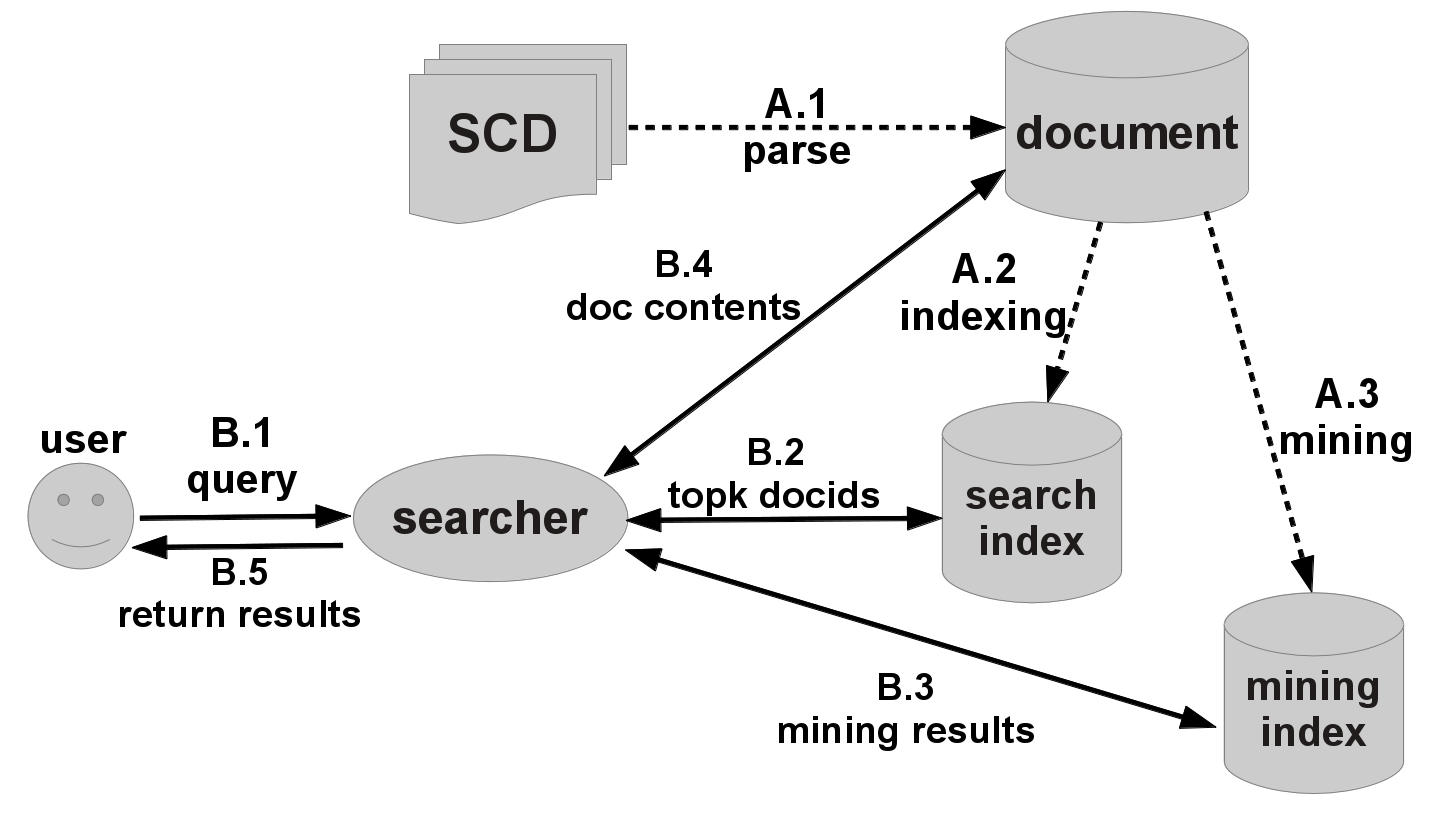
\includegraphics[width=.8\textwidth]{Figures/sf1_workflow.png}
\caption{SF1 Workflow}\label{fig:sf1_workflow}
\end{figure}

\section{Build Process}

\begin{enumerate}
\item[A.1] \textbf{SCD parsing}. The input of the building process are text files in the \textbf{SCD} format.
They are parsed into documents, and each document consists of pairs of property name and value. The documents are stored by \textbf{document manager} which
is a document oriented nosql actually.

\item[A.2] \textbf{indexing}. For those properties which are configured for search, their property values are used to build the \textbf{search index}.
To satisfy different search requirements, there are three kinds of search indices. They are \textbf{disk based index} for general search,
\textbf{suffix index} for fast fuzzy search in pure memory and \textbf{zambezi index} for fast boolean search in pure memory. For the sake of 
conveniences on implementation, \textbf{suffix index} belongs to mining procedure actually although it has the semantic of \textbf{search}. The indexing
procedure co-work with \textbf{SCD parsing} such that whenever a document is inserted into the nosql store, corresponding indices have been setup.

\item[A.3] \textbf{mining}. For those properties which are configured for mining features, such as groupby, attrby, etc,
their property values are used to build the \textbf{mining index}. \textbf{SF1R} has contained tens of mining features through \textbf{mining} procedure,
while in this technical report, only search as well as navigation relevant ones are mentioned due to frequent usage. \textbf{Mining} procedure is performed
after \textbf{indexing} stage, it directly get raw data from \textbf{document manager} and dispatch them into different kinds of mining components according
to configuration.

\end{enumerate}

\section{Query Process}

\begin{enumerate}
\item[B.1] Given the user query, it would be tokenized into \textbf{terms}.
The tokenization methods include minimum match, maximum match, maximum entropy and CRF.

\item[B.2] These terms are searched among the search index to get candidate docids.
Each candidate would be assigned with a score, calculated by ranking methods such as TF-IDF, BM25, product ranking, etc.
Finally the candidates with top scores are extracted as \textbf{topk docids}.

\item[B.3] If the request has parameters on mining features, those candidate docids are searched among the mining index to get \textbf{mining results}.

\item[B.4] The topk docids are searched among the document manager to get the \textbf{document contents}.

\item[B.5] Finally the \textbf{search results} are returned to user.

\end{enumerate}

\section{Architecture}
The architecture of \texttt{SF1R} could be seen from figure \ref{fig:sf1_architecture}, this is an overview for the system running on single machine. \texttt{SF1R}
provides unified implementation to be deployed on either single node or search cloud just via adjusting configurations. There are two separated processes within \texttt{SF1R}
system---the search engine server itself and the reverse proxy which is based on \texttt{nginx}, as shown in \ref{fig:sf1_architecture}.
\begin{figure}[htbp]
  \centering
    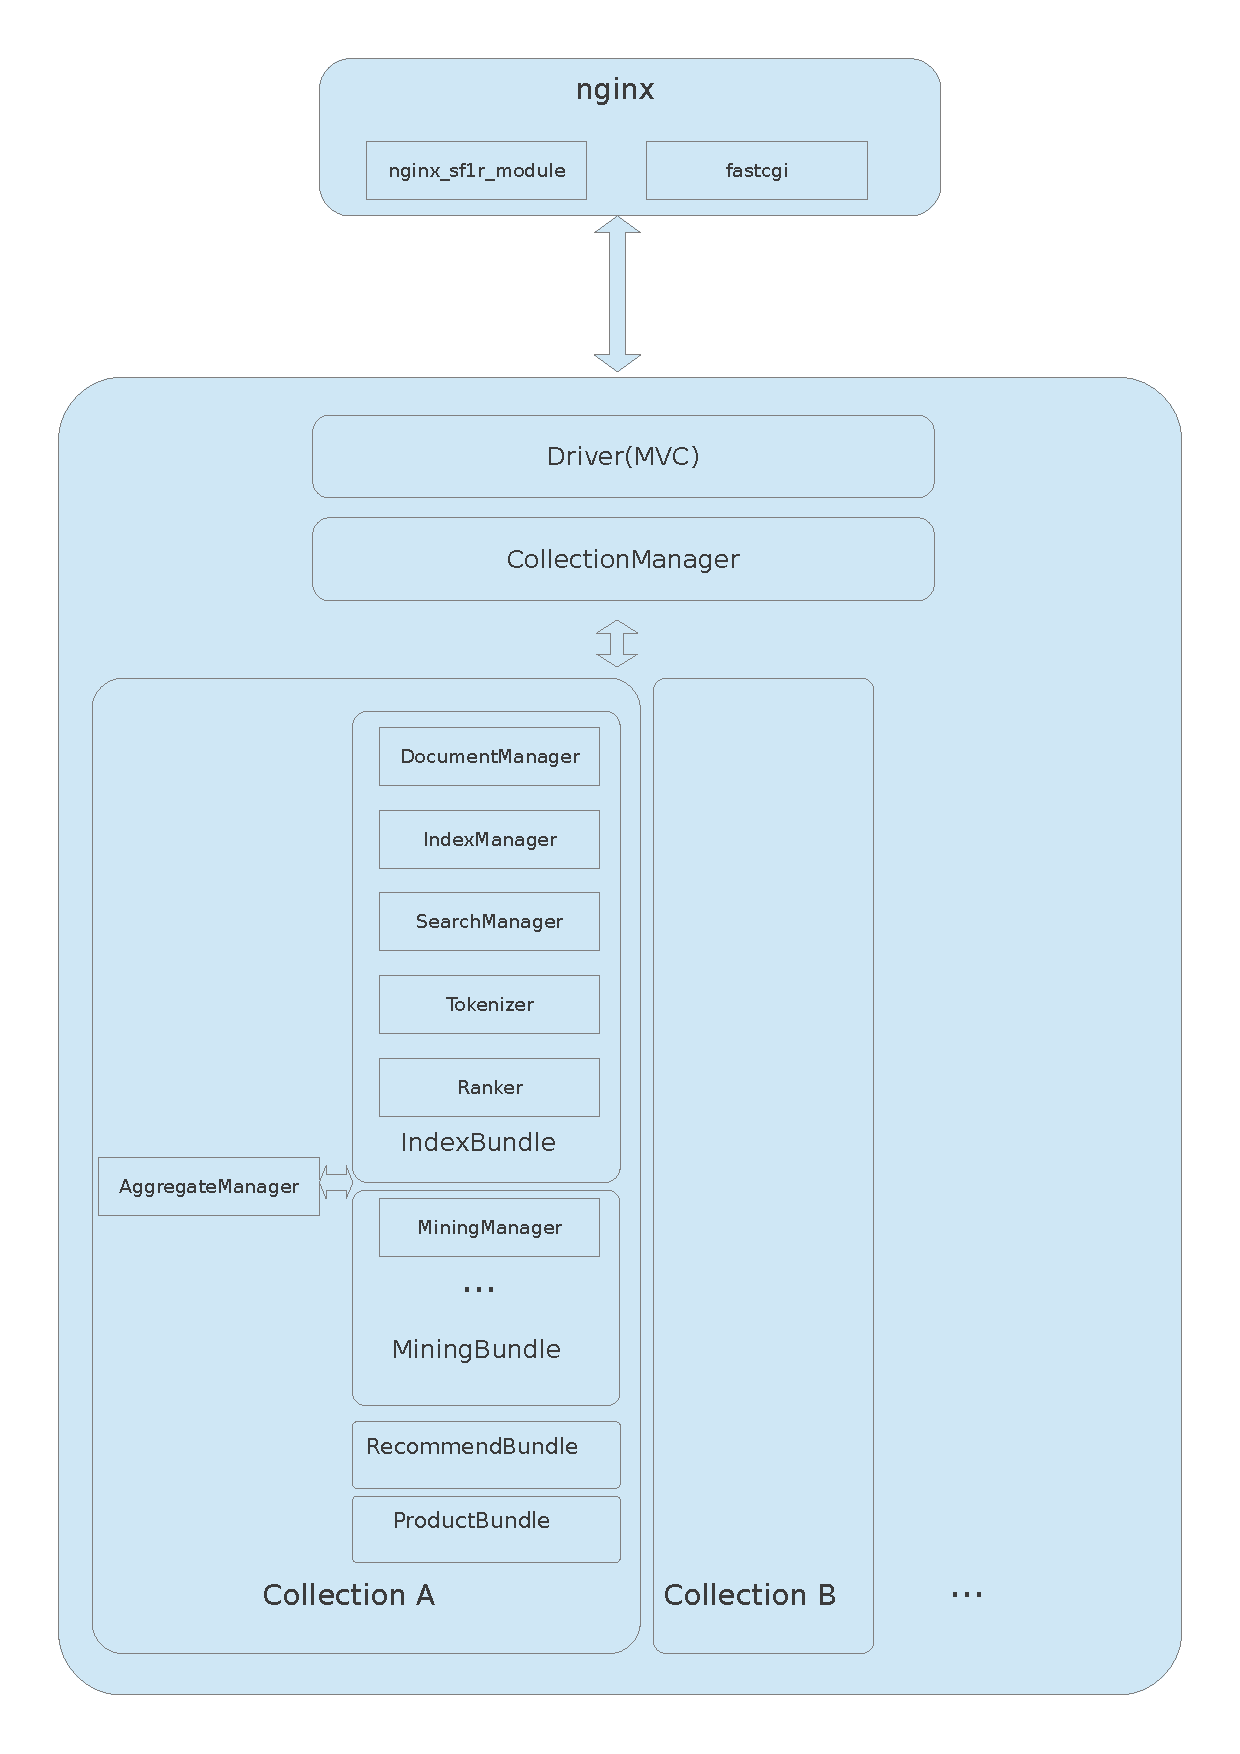
\includegraphics[width=.7\textwidth]{Figures/sf1.pdf}
    \rule{35em}{0.5pt}
  \caption[Architecture of SF1R]{Architecture of SF1R---Non-distributed On Single Machine}
  \label{fig:sf1_architecture}
\end{figure}

\subsection{Key Components}
\begin{itemize}
 \item nginx---This is the customized version to be tailed to connect with \texttt{SF1R} server, such that \texttt{http} based API could be provided to applications. As a result, 
 the client of \texttt{SF1R} is language independent. There are two kinds of mechanism for the connnection between nginx and the search engine server:
  \begin{itemize}
   \item nginx module---The nginx ecosystem delivers a flexible mechanism such that any customized module could be developed for reverse upstream servers \cite{nginx}. The nginx module runs within
   the same process together with nginx worker, as a result, when nginx is going to be connected to multiple \texttt{SF1R} servers, this is not a recommended approach for concurrency consideration.
   \item fact cgi---This is a traditional upstream mechanism for nginx ecosystem, while we have made customization to it as well such that each fast cgi process could be used to serve
   any requests routing to any remote \texttt{SF1R} server. Fast cgi is a preferred approach when deploying \texttt{SF1R} in distributed environment.
  \end{itemize}

 \item Driver---This is the network encapsulation within \texttt{SF1R} server. We borrowed the idea from web application to introduce the \texttt{MVC} pattern, such that application
 logic could be developed flexiblely based on the \texttt{Driver} layer.
 \item CollectionManager---\texttt{Collection} is the fundamental concept within \texttt{SF1R}, corresponding definition in database is \texttt{table}. The collection could be created,
 destroyed, started, as well as stopped dynamically through \texttt{CollectionManager}, just like how database manages its tables. Each request sent to \texttt{SF1R} should specify its
 target collection, such that the request could be routed correctedly.
 \item Bundle---The concept of \texttt{bundle} comes from Java enterprise community---\texttt{OSGI} \cite{osgi}. The introduction of bundle is to make the architecture more flexible and
 seperated, each collection will have its own bundle instances to make sure total separation. The existing bundles include:
  \begin{itemize}
   \item IndexBundle---It has contained core components during indexing, such as DocumentManager for data archiving, IndexManager for archive indexing,
   SearchManager and a series rankers for search operations.
   \item MiningBundle---All mining features are included in this bundle.
   \item RecommendBundle---\texttt{SF1R} has also delivered a feature to provide unified search engine and recommendation engine. RecommendBundle is for the purpose of recommendation,
   currently, the core algorithm of this engine is based on incremental item-item collaborative filtering.
  \end{itemize}
 \item AggregateManager---This is a fundamental building block for distributed search. \texttt{SF1R} provides single implementation on distributed and non-distributed version. AggregateManager
 is the key encapsulation for this unified behavior, it means, when deployed on single machine, it could be looked on as a transparent layer to serve requests, while when deployed 
 distributedly, it will have different behaviors depending on whether that node is \texttt{Master} or \texttt{Worker}:
  \begin{itemize}
   \item Worker is the node serving practical requests over its local data.
   \item Master is the node to dispatch and aggregate requests from multiple workers.
   \item Master and Worker could be deployed either together or remotely --- just via adjusting configurations.
  \end{itemize}

\end{itemize}


\chapter{Navigation---Groupby/Attrby}
\lhead{Chapter 2. \emph{Navigation---Groupby/Attrby}} % this is for the header on each page - perhaps a shortened title

Groupby means "Group by Property", it groups search results into each property value. Attrby means "Group by Attribute", it groups search results according to each attribute value.
Such kinds of grouping is frequently used in search navigation for such vertical searchs as e-commerce,..,etc. 

\section{Index Structure}
\label{GroupIndex}

The index structure for both Groupby and Attrby search is based on a forward index, as shown in \ref{fig:group_index}. 
In order to save the memory cost, the property value strings are mapped to ids. For each docid, we need to store an array of value ids, as the number of value ids might be 
different for each docid. The group index structure consists of two tables, one is \textbf{index table}, the other is \textbf{value id table}.
The \textbf{index table} stores index (or value id) for each docid. If this doc has only one value id, then it stores the value id direcly.

While if it has multiple value ids, then it stores the index in the \textbf{value id table}.In order to differentiate these two cases, we use the most significant bit.
That is, bit 0 for the case of single value id, and bit 1 for the other case.  In the \textbf{value id table}, the 1st entry is the number of value ids.
The following entries are each value id for the doc.

\begin{figure}[htp]
\centering
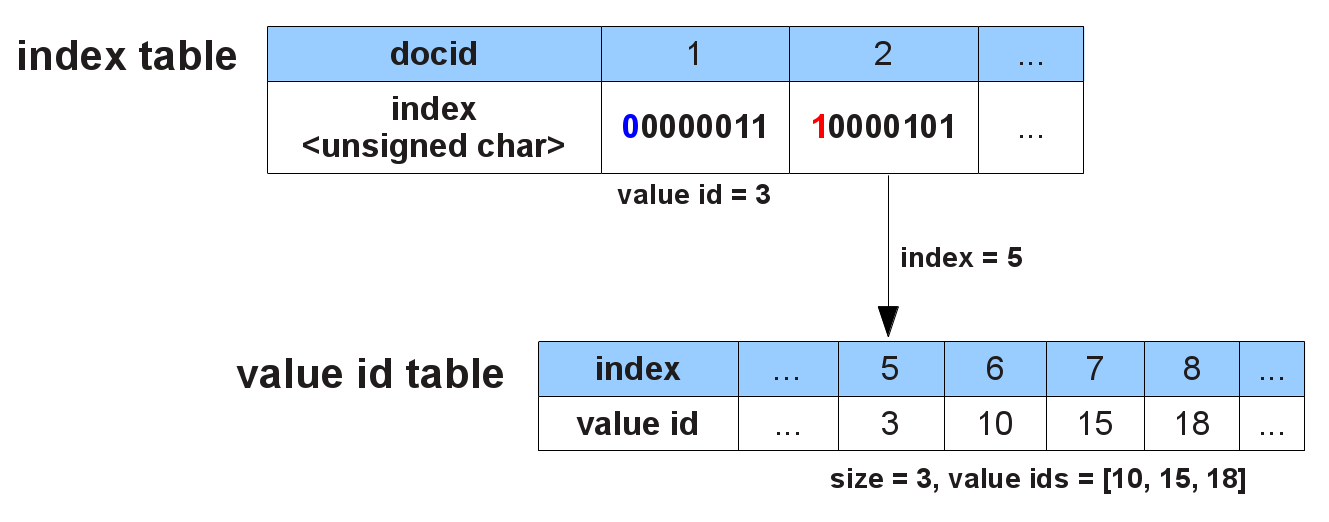
\includegraphics[width=0.8\textwidth]{Figures/group_index.png}
\caption{Group Index Example}\label{fig:group_index}
\end{figure}

In the example of figure \ref{fig:group_index}, the index type is parameterized as unsigned char. The docid 1 has only one value id (3), and the docid 2 has three value ids 
(10, 15 and 18).


\section{SCD Format}

The Groupby search requires corresponding property type to be string, it supports hierarchical values. Below is its SCD format:
\begin{lstlisting}
<PropertyName>A>B>C,D>E>F...
\end{lstlisting}

\begin{itemize}
\item The \verb!PropertyName! is the property name which needs group results;
\item The property could contain multiple values, each separated by comma \verb!,! or semicolon \verb!;!
\item If the value has parent value, you need to specify the whole path from root to leaf node, each separated by symbol \verb!>!
\item If one attribute name contains multiple values, such as A, B and C, each value is separated by the vertical line \verb!|!, for example, \verb!name:A|B|C!
\item In property values, if there is any embedded character of comma \verb!,!, semicolon \verb!;!, symbol \verb!>! or double-quote \verb!"!,
the whole value must be surrounded by double-quotes.
And the embedded double-quotes must each be represented by a pair of consecutive double quotes.
For example, if the property value contains values on three levels. The root value is John, Mark. The 2nd level value is 1+1>2. The 3rd level value is "Mary".
Then you need to specify it as \verb!"John, Mark">"1+1>2">"""Mary"""! in SCD file

Please note that all of the above punctuations and symbols are half width.

\end{itemize}

The Attrby search also requires the attribute property type to be string with such kinds of format:
\begin{lstlisting}
<PropertyName>name:value,name:value...
\end{lstlisting}

\begin{itemize}
\item The \verb!PropertyName! is the property name which contains pairs of attribute name and value.

\item Each pair of attribute name and value is separated by the comma \verb!,!

\item Attribute name and value are separated by the colon \verb!:!

\item If one attribute name contains multiple values, such as A, B and C, each value is separated by the vertical line \verb!|!, for example, \verb!name:A|B|C!

\item In attribute name or value, if there is any embedded character of above delimiters \verb!,:|! or double-quote \verb!"!, the whole attribute name or value must be surrounded by double-quotes.
And the embedded double-quotes must each be represented by a pair of consecutive double quotes \verb!""!.
For example, if the attribute name or value is \verb!John, Mark: "Mary" | Tom!, you need to specify it as \verb!"John, Mark: ""Mary"" | Tom"! in SCD file.

Please note that all of the above punctuations \verb!,:|"! are half width.

\end{itemize}


\section{Configuration}
\subsection{Groupby Search}
\begin{itemize}
\item In collection config file, such as \verb!config/example.xml! in sf1r-engine, for the property in \verb!DocumentSchema!,
if you need group results on this property (the property type must be string, int, float or datetime),
you have to configure it in \verb!MiningBundle/Schema/Group!.

\item If the property type is int or float, you also need to configure it as filter property in \verb!IndexBundle!.

\item For the property type of int and float, it's unnecessary to build group index data.

\item While for the property type of string and datetime, it would build group index data when each time SCD is indexed.
Normally, it starts from the last doc id when last time group index data is built.

\item If the string property is configured as \verb!<IndexBundle><Schema><Indexing ... rtype="y"/>!,
then for this RType string property, it would rebuild its whole group index data when each time SCD is indexed.

\item For other properties, if you want to rebuild the whole group index data when each time SCD is indexed,
you need to configure the "rebuild" attribute to "y". For example, \verb!<Group><Property name="Category" rebuild="y"/>!.

\end{itemize}

For example:

\begin{lstlisting}
<DocumentSchema>
  ...
  <Property name="Category" type="string" />
  <Property name="Price" type="float" />
  <Property name="PlayTime" type="datetime" />
</DocumentSchema>

<IndexBundle>
  <Schema>
    <Property name="Price">
      <Indexing filter="yes" multivalue="no" doclen="yes" tokenizer="" rankweight="0.1" />
    </Property>
    ...
  </Schema>
</IndexBundle>

<MiningBundle>
  <Schema>
    ...
    <Group>
      <Property name="Category" />
      <Property name="Price" />
      <Property name="PlayTime" />
    </Group>
  </Schema>
</MiningBundle>
\end{lstlisting}

\subsection{Attrby Search}
In collection config file, such as "config/example.xml" in sf1r-engine, for the property which contains attribute names and values,
you have to add it in \textbf{MiningBundle/Schema/Attr}. Please note that at most one property is allowed in \textbf{Attr} configuration.

If you want to exclude some attribute names, you need to configure them into \textbf{Exclude}.

For example:

\begin{lstlisting}
<DocumentSchema>
  ...
  <Property name="Attribute" type="string" />
</DocumentSchema>
...
<MiningBundle>
  <Schema>
    ...
    <Attr>
      <Property name="Attribute" />
      <Exclude name="ISBN" />
    </Attr>
  </Schema>
</MiningBundle>
\end{lstlisting}


\chapter{Disk Based Index}
\lhead{Chapter 3. \emph{Disk Based Index}} % this is for the header on each page - perhaps a shortened title
\section{Introduction}
Disk Based Inverted Index is our first index libary to serve all \texttt{iZENECloud} products with efficient control of memory consumption together with a high performance. Compared
with other open source solutions such as Lucene \cite{lucene}, the fundamental architecture is similar while we have several extra highlights. As shown in figure \ref{fig:voc1}, basic
inverted index is composed of two parts: vocabulary and posting lists. The vocabulary contains all indexed terms and its pointer to cooresponding posting list. The major design issues
are discussed in the following section. Within \texttt{SF1}, corresponding component of this disk based inverted index is \texttt{IndexManager}.
\begin{figure}[htp]
\centering
\centerline{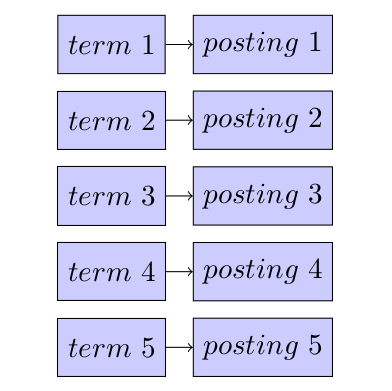
\includegraphics[width=.4\textwidth]{Figures/voc1.png}}
\caption{Inverted Index}\label{fig:voc1}
\end{figure}

\section{Design Issues}
\subsection{Vocabulary Design}
In order to reduce memory consumption, we've adopted an engineering trick of \texttt{Sparse Binary Search}. As we can see from figure \ref{fig:voc1}, the vocabulary itself 
is nothing more than a hash map, since we store term ids within the vocabulary, each entry of the vocabulary has a fixed length. During search process, if we do not load any 
entries of the vocabulary into memory, for each query, we will have to need $O(log|Voc|))$ disk accesses to locate posting lists, while when sparse binary search is applied, 
we could reduce the disk accesses to $O(1)$ instead of $O(log|Voc|))$, as seen in figure \ref{fig:voc2}.

\begin{figure}[h!]
\centerline{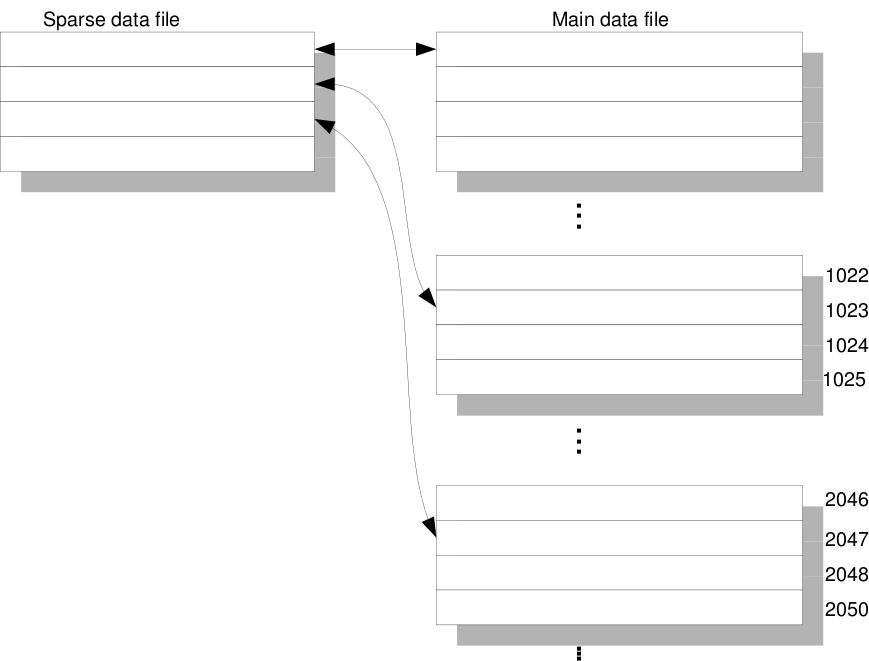
\includegraphics[width=0.6\textwidth]{Figures/voc2.png}}
\caption{Sparse Binary Search}\label{fig:voc2}
\end{figure}

Via storing each 512th entry of the vocabulary data in memory, and then ensuring that the initial delta value of the binary search algorithm is a power of 512, all comparisons required for the binary search will use the data
available in main memory. This optimization requires $O(log|Voc|/512))$ main memory usage.

When using the sparse data described above, the first phrase of the binary search algorithm can determine two 512 entry areas of the vocabulary where the record searched for may reside. Since the overhead of positioning
the disk heads for a read operation is high relative to the time a disk transfer, it will pay off to buffer these 1023 entries when the delta gets below the value of 512. 

\subsection{Index Construction}\label{indexCon}
IndexManager is designed to support both on-line indexing, which is mainly used for real-time search, as well as traditional off-line indexing. The user of IndexManager could designate either of these two indexing modes easily 
just by a configuration parameter. The index construction processes for each of these two modes are totally different:
\begin{itemize}
 \item The real-time indexing requires the inverted index for a certain document to be able to search immediately just after that document is indexed. 
 \item The offline indexing could build index for a batch of documents at one time for a much faster indexing speed.
\end{itemize}

The real-time indexing has a much higher design complexity than the offline one. In order to make the design of both two indexing modes into an overall integrity, we introduce a new concept---\texttt{Index Barrel},
which means the index of a batch of documents. As a result, for the overall indices, we might have multiple index barrels, each of which contain cooresponding documents:
\begin{itemize}
 \item For the offline mode, index for all documents to be indexed will be encapsulated into a single index barrel.
 \item The index construction process for on-line mode will be discussed in the following sub section \ref{indexcon-merge}.
\end{itemize}

In following subsections, we will describe the detailed index construction process for both two modes respectively.

\subsubsection{Off-line Index Construction} \label{indexcon-offline}
Off-line index means the index for the documents could not be searched during indexing. In this case, we could design a very efficient process to make the batch indexing extremely fast:
The inputs of IndexManager is a series of documents, each of which is nothing more than a series of terms, each of which is composed of both term id and term position. As a result, we could look on the 
batch inputs as a series of such kinds of data structures:
\begin{lstlisting}[language=C]
struct Term
{
    uint32_t docId;
    uint32_t termId;
    uint32_t termPosition;
};
\end{lstlisting}
And we need all of these inputs to be sorted according to the priority of \texttt{termId},\texttt{docId} and \texttt{termPosition}, the key design issue is how could we sort the data inputs efficiently ?

\begin{figure}[h!]
\centerline{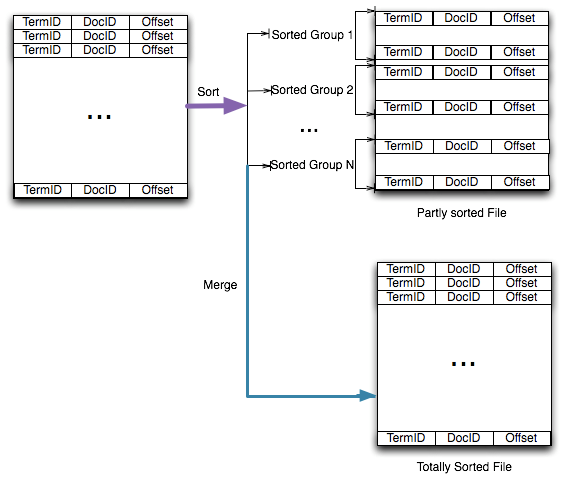
\includegraphics[width=0.6\textwidth]{Figures/izene_sort.png}}
\caption{Offline Index Sorting Process}\label{fig:indexcon-sort}
\end{figure}


Figure \ref{fig:indexcon-sort} has illustrated the sorting process adopted by IndexManager---it's an improved version for \texttt{merge-sort} process that is frequently used in external sorting algorithms:
\begin{itemize}
 \item Firstly, IndexManager will create a memory buffer, say 100M, to accumulate the inputed data.
 \item When the memory buffer is full, a memory sort will be performed for those contained data, and the results will be written to an intermediate file.
 \item The above steps will be continuously looped until there are no documents to be indexed. As a result, the intermediate file is a partly sorted file.
 \item A final merge sort will be performed based on the previously mentioned intermediate file.
\end{itemize}

Such merge sort based process is extremely efficient. For each batch off-line indexing process, a single index barrel is generated, while if we have several index operations, 
eg: we index 1M documents, 100k documents, and 10k documents sequentially, we then have 3 index barrels. How to manage these three index barrels have closely relation with the
on-line index construction mode, and we will discuss this issue in the next sub section.


\subsubsection{Merge Based Index Construction} \label{indexcon-merge}
During past years, great advances have been achieved to build an off-line index, which could not provide query service during the process of index construction. However, with the boom of the web pages' count number, 
to provide search ability during indexes construction has been more and more urgent, therefore how to maintain on-line index is the current research hotspot on indexing problems. There are three kinds of index construction
method: In-place, Re-build, and Re-merge\cite{lester2004pvr}. For In-place update strategy, documents are accumulated in main memory. Then, once main memory is exhausted, the existing on-disk index is combined with 
the in-memory index by appending each posting list from the in-memory index to the corresponding list in the on-disk index; The Re-build algorithm constructs a new index from the current entire collection; For the Re-merge 
update strategy, once main memory is exhausted, a merge event is triggered, and the entire on-disk index is read sequentially and merged with the in-memory index, then written to a new location to form a new on-disk index
that immediately replaces the old one. According to the experiments of \cite{lester2004pvr}, in most cases, Re-merge strategy would perform better than the other two approaches. 

\begin{figure}[h!]
\centerline{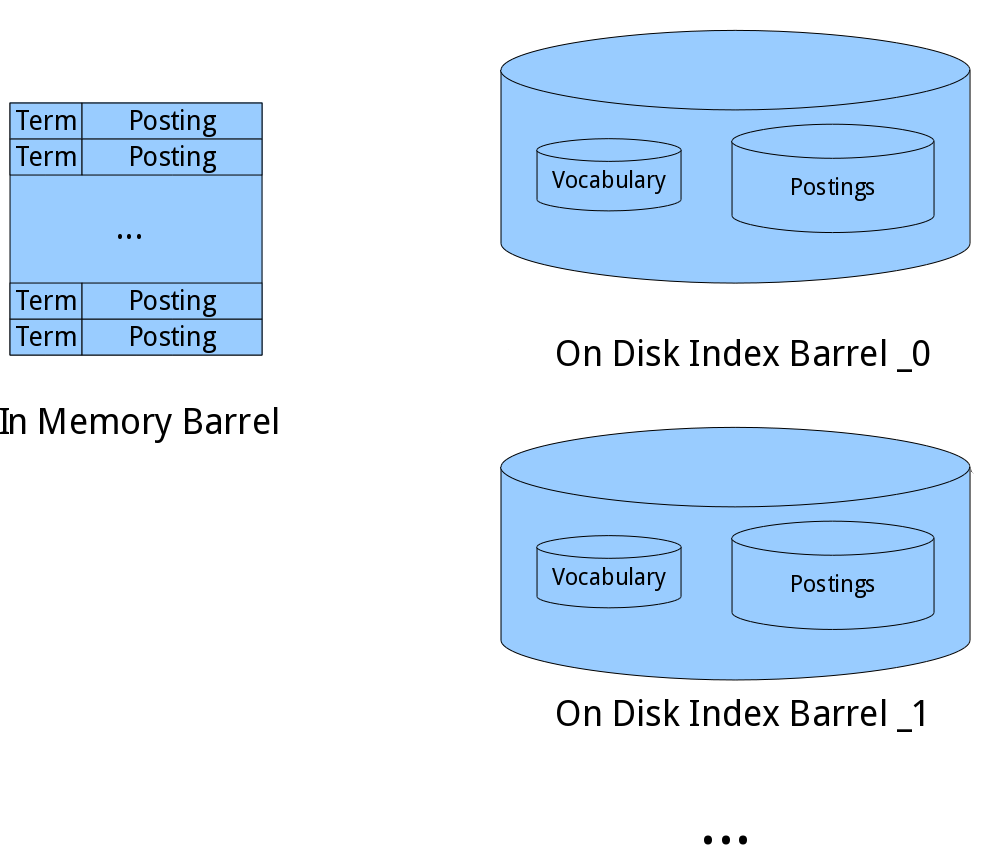
\includegraphics[width=0.4\textwidth]{Figures/barrel1.png}}
\caption{Index Barrels for On-line Indexing}\label{fig:indexcon-barrel1}
\end{figure}

Figure \ref{fig:indexcon-barrel1} shows the on-line indexing process: Unlike offline indexing mode, there's no sorting process for a batch of documents, instead, inverted index is built for each document as soon as that 
document is pass to IndexManager. There's a memory pool maintained by IndexManager, as soon as index for documents has used up that memory pool, all of the index data will be flushed to disk to form an on disk
index barrel, named start from $_0$, $_1$,...,etc, and then the memory pool could contain index for new documents, obviously, the in-memory index is another index barrel.  All of the on disk index barrels as well as 
the in-memory index barrel could be searched start from scratch, so we could provide real-time search utilities in this indexing mode.

The key design issue for this kind of index construction is how we manage these index barrels: because in this kind of indexing mode, we might generate much more index barrels than offline mode: as soon as the memory
pool is used up, we are going to generate a new index barrel. Given a 128M memory pool, we can only index 10k documents approximately. As a result,for a given 5M corpus, we might generate hundreds of index barrels. 
We can not keep the number of index barrels large, or else the search performance will be affected. We also can not merge those index barrels frequently, or else the indexing performance will be affected. The Dynamic 
Balancing Tree algorithm \cite{guo2007eli} is used for one of the index merging policy, which provides an index merging algorithm that supports on-line index maintenance. 
\par
DBT\cite{guo2007eli} index construction strategy is a kind of Re-merge algorithm and performs the best among all available schemes.  A DBT is an m-way tree, each node of which is a sub-index. The tree is divided into $H$ layers from bottom to top. At layer $k$, the number of nodes is either zero, or is less than m. Let $\mathbf{E}_{k,j}$ be the capacity of node $j, 0\leq j<m-1$, at layer $k, 0\leq k<H$, a constraint of the number of documents in one node of layer $k$ is given by:
\begin{equation}
c^{k}\leq \epsilon_{k,j}<c^{k+1}
\end{equation}

When the size of each node in layer $k$ satisfy the above equation, the tree is balanced. When the number of nodes in the layer $k$ is equal to or greater than $m$, a merge event is triggered, resulting a new sub-index. The newly created sub-index will be placed into layer $k+1$. If the tree is balanced and a sub-index merge operation is only performed on one layer, the efficiency of merging process can be guaranteed.   According to the experiments in \cite{guo2007eli}, choosing the param value of $m=c=3$ offers better indexing performance. \par

In the implementation, the index is organized into several barrels. One barrel refers to one node in the DBT tree. When constructing the index, the postings will be built up in memory at first, when the memory has been exhausted, these postings will be flushed to one barrel, the layer of which in the DBT tree could be computed by the above equation according to the document number that have been indexed in this barrel. If the number of barrels of a certain layer satisfy the merge condition described above, these barrels will be merged together to form a new barrel, and the old barrels will be deleted. Therefore, merge operation has been limited within several barrels since it is an expensive process, and the total barrels could be controlled because too many barrels will effect the query performance. What's more, all of the barrels could be merged into one monad manually to provide better query performance.


IndexManager provides flexible encapsulation so that different kinds of merge policies could be implemented easily. Except for DBT merge policy, IndexManager also has other merge policies, such as multi-way merge, 
which is used by Lucene\cite{lucene}, and optimize-merge, which is used to merge all index barrels into single index barrel for best index search performance. Different kinds of index merge algorithm is shared by both online-indexing
and off-line index, and the user of IndexManager could config to choose the suitable merge algorithm. Figure \ref{fig:indexcon-barrel2} gives a simple graph show for these three different kinds of merge policies.

\begin{figure}[h!]
\centerline{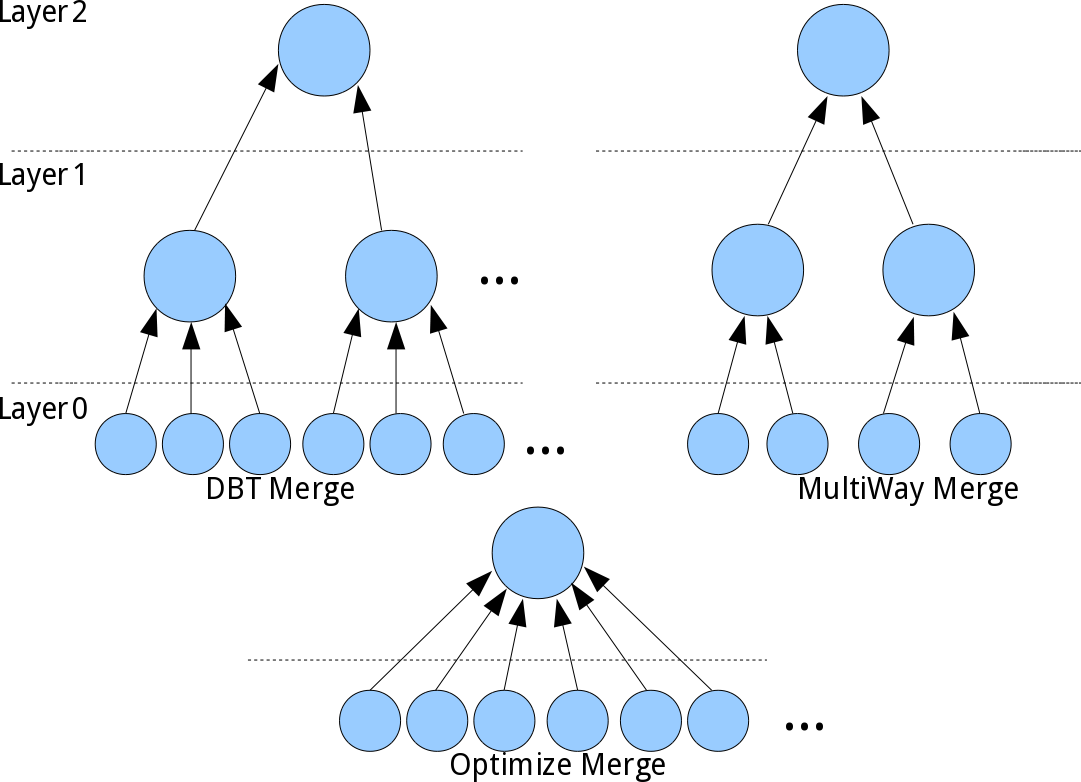
\includegraphics[width=0.6\textwidth]{Figures/barrel2.png}}
\caption{Index Barrels Merge Policies}\label{fig:indexcon-barrel2}
\end{figure}


\subsection{Index Compression}
Compressioin is a very effective solution to struggle with disk IO. There exists a trade off between the compressibility and decoding speed. Higher compression ratio would always lead to slower decoding, if it is too slow, then query performance will be effected. D-gap together with variable length are adopted to compress the index, because it is very fast to decode, and can reduce the index size to about $\frac{1}{2}$ to $\frac{1}{4}$ of the original. It is a mature scheme and has been adopted by most of the existing \texttt{IR} frameworks. This compression solution is the default policy for IndexManager. Besides, we have also implemented the state-of-art index compression scheme, such as \texttt{pForDelta}, a composition of \texttt{pForDelta} and \texttt{S16}, the details could be found in \cite{zukowski2006ssr}, \cite{zhang2008pci},\cite{yan2009inverted},and \cite{yan2009compressing}. These state-of-the-art
compression schemes have also been adopted by the latest \texttt{Google} web search, as a result, our IndexManager has already kept up with the cutting edge of index design area. Since these compression solutions all perform decoding and encoding operations in a batch way, their detailed design within IndexManager is totally different with the variable length solution, we will describe the details in the later section.

\subsection{Index Deletion}
IndexManager uses a bitmap file to indicate the deleted documents. However, if there are too many deleted documents, it will affect the search performance a lot. In that case, IndexManager could utilize the index merger to generate
the new index, within which those delete documents will not appear any more. Another issue is the requirement for supporting \texttt{Document Updating} semantics, in such cases, the updated documents will be assigned with new doc 
ids before they are passed to IndexManager, so that the \texttt{Document Updating} semantics is just a simple composition of \texttt{Document Deletion} and \texttt{Index Document}.

\subsection{B-Tree Index}
When indexing documents, some kinds of data is not suitable to be stored within inverted index, such as date and time, number, etc, because range query is required over vocabulary, 
this is more usual under search filtering. Within \texttt{SF1}, we use B-Tree index for such purpose, the output for any conditional search filtering is a bitmap to be intersected
with results got from inverted index.

\section{Architecture}
Following description for architecture design only focuses on the inverted index parts. There are overall three components for inverted index design:
\begin{itemize}
 \item IndexWriter, which is used to build index---both online and offline.
 \item IndexMerger, which is used to merge index barrels.
 \item IndexReader, which is used to perform search utilities.
\end{itemize}
We will describe each of them in the following sections.


\subsection{IndexWriter}

Figure \ref{indexWriter} shows the hierarchy of IndexWriter of how to form a single barrel index. 

\begin{figure}[h!]
\centerline{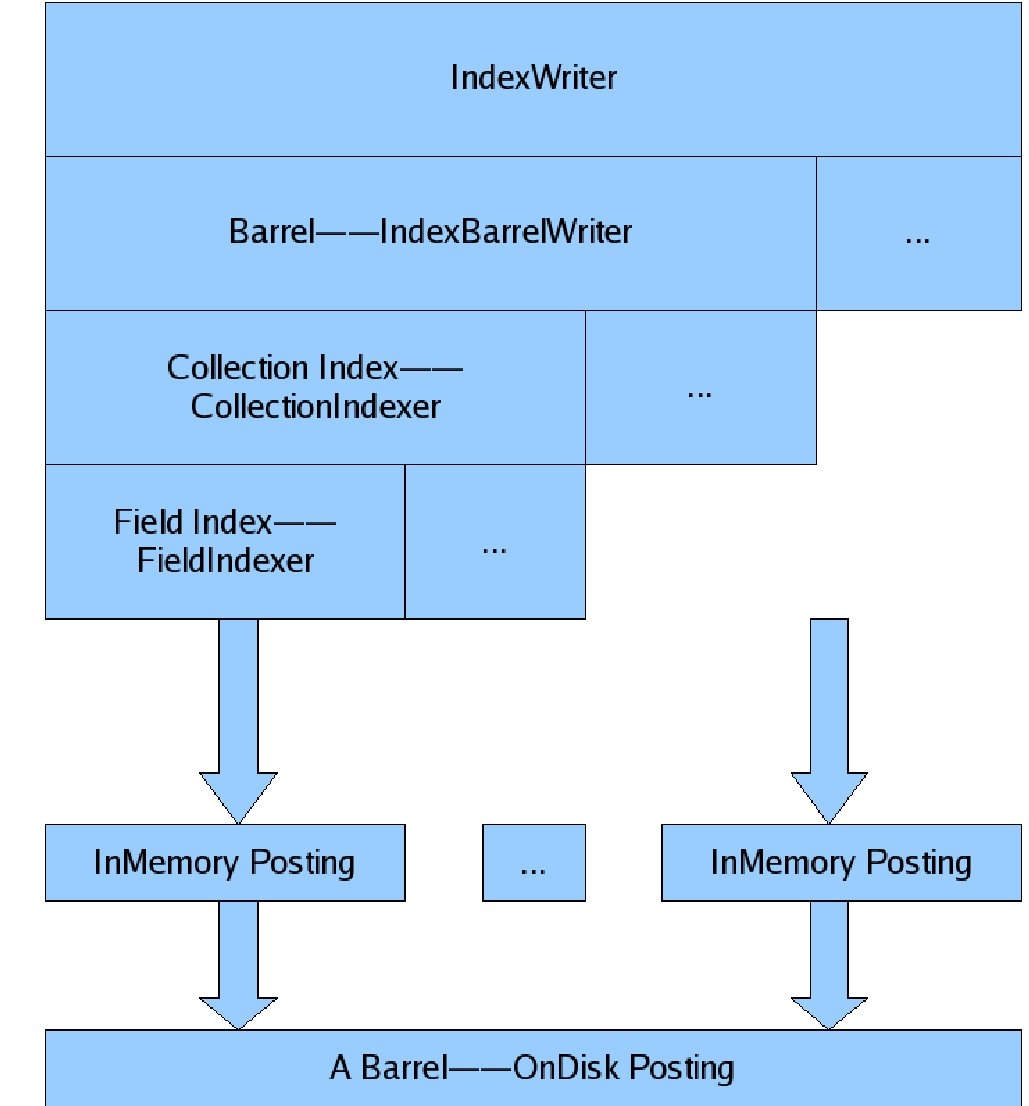
\includegraphics[width=0.4\textwidth]{Figures/indexWriter.jpg}}
\caption{Hierarchy of IndexWriter}\label{indexWriter}
\end{figure}


\par
As has been shown above, IndexBarrelWriter is in charge of flushing index into one barrel. Internally, it contains a serial instances of CollectionIndexer, each of which corresponds to one collection solely. Inside a CollectionIndexer, there are several FieldIndexers, which takes charge of building index within its corresponding Field. After Indexer starts up, the instances of CollectionIndexer and FieldIndexer will be created according to DocumentSchema that have been initialized by the user of IndexManager. In our document model, each document contains several configurable fields, such as \texttt{Title},\texttt{Content},...,etc. Index for each field is independent from each other.  FieldIndexer will build index of one field
of a collection. There are two kinds of posting lists in the system: document-frequency posting and position posting. The former stores document id and frequency of a certain term that has appeared in that document. The latter stores all the term position information of a certain term in the document. 
Suppose we only have general variable length compression scheme, figure \ref{barrelFormat} gives a detailed description of what a single barrel index contains:

\begin{figure}[h!]
\centerline{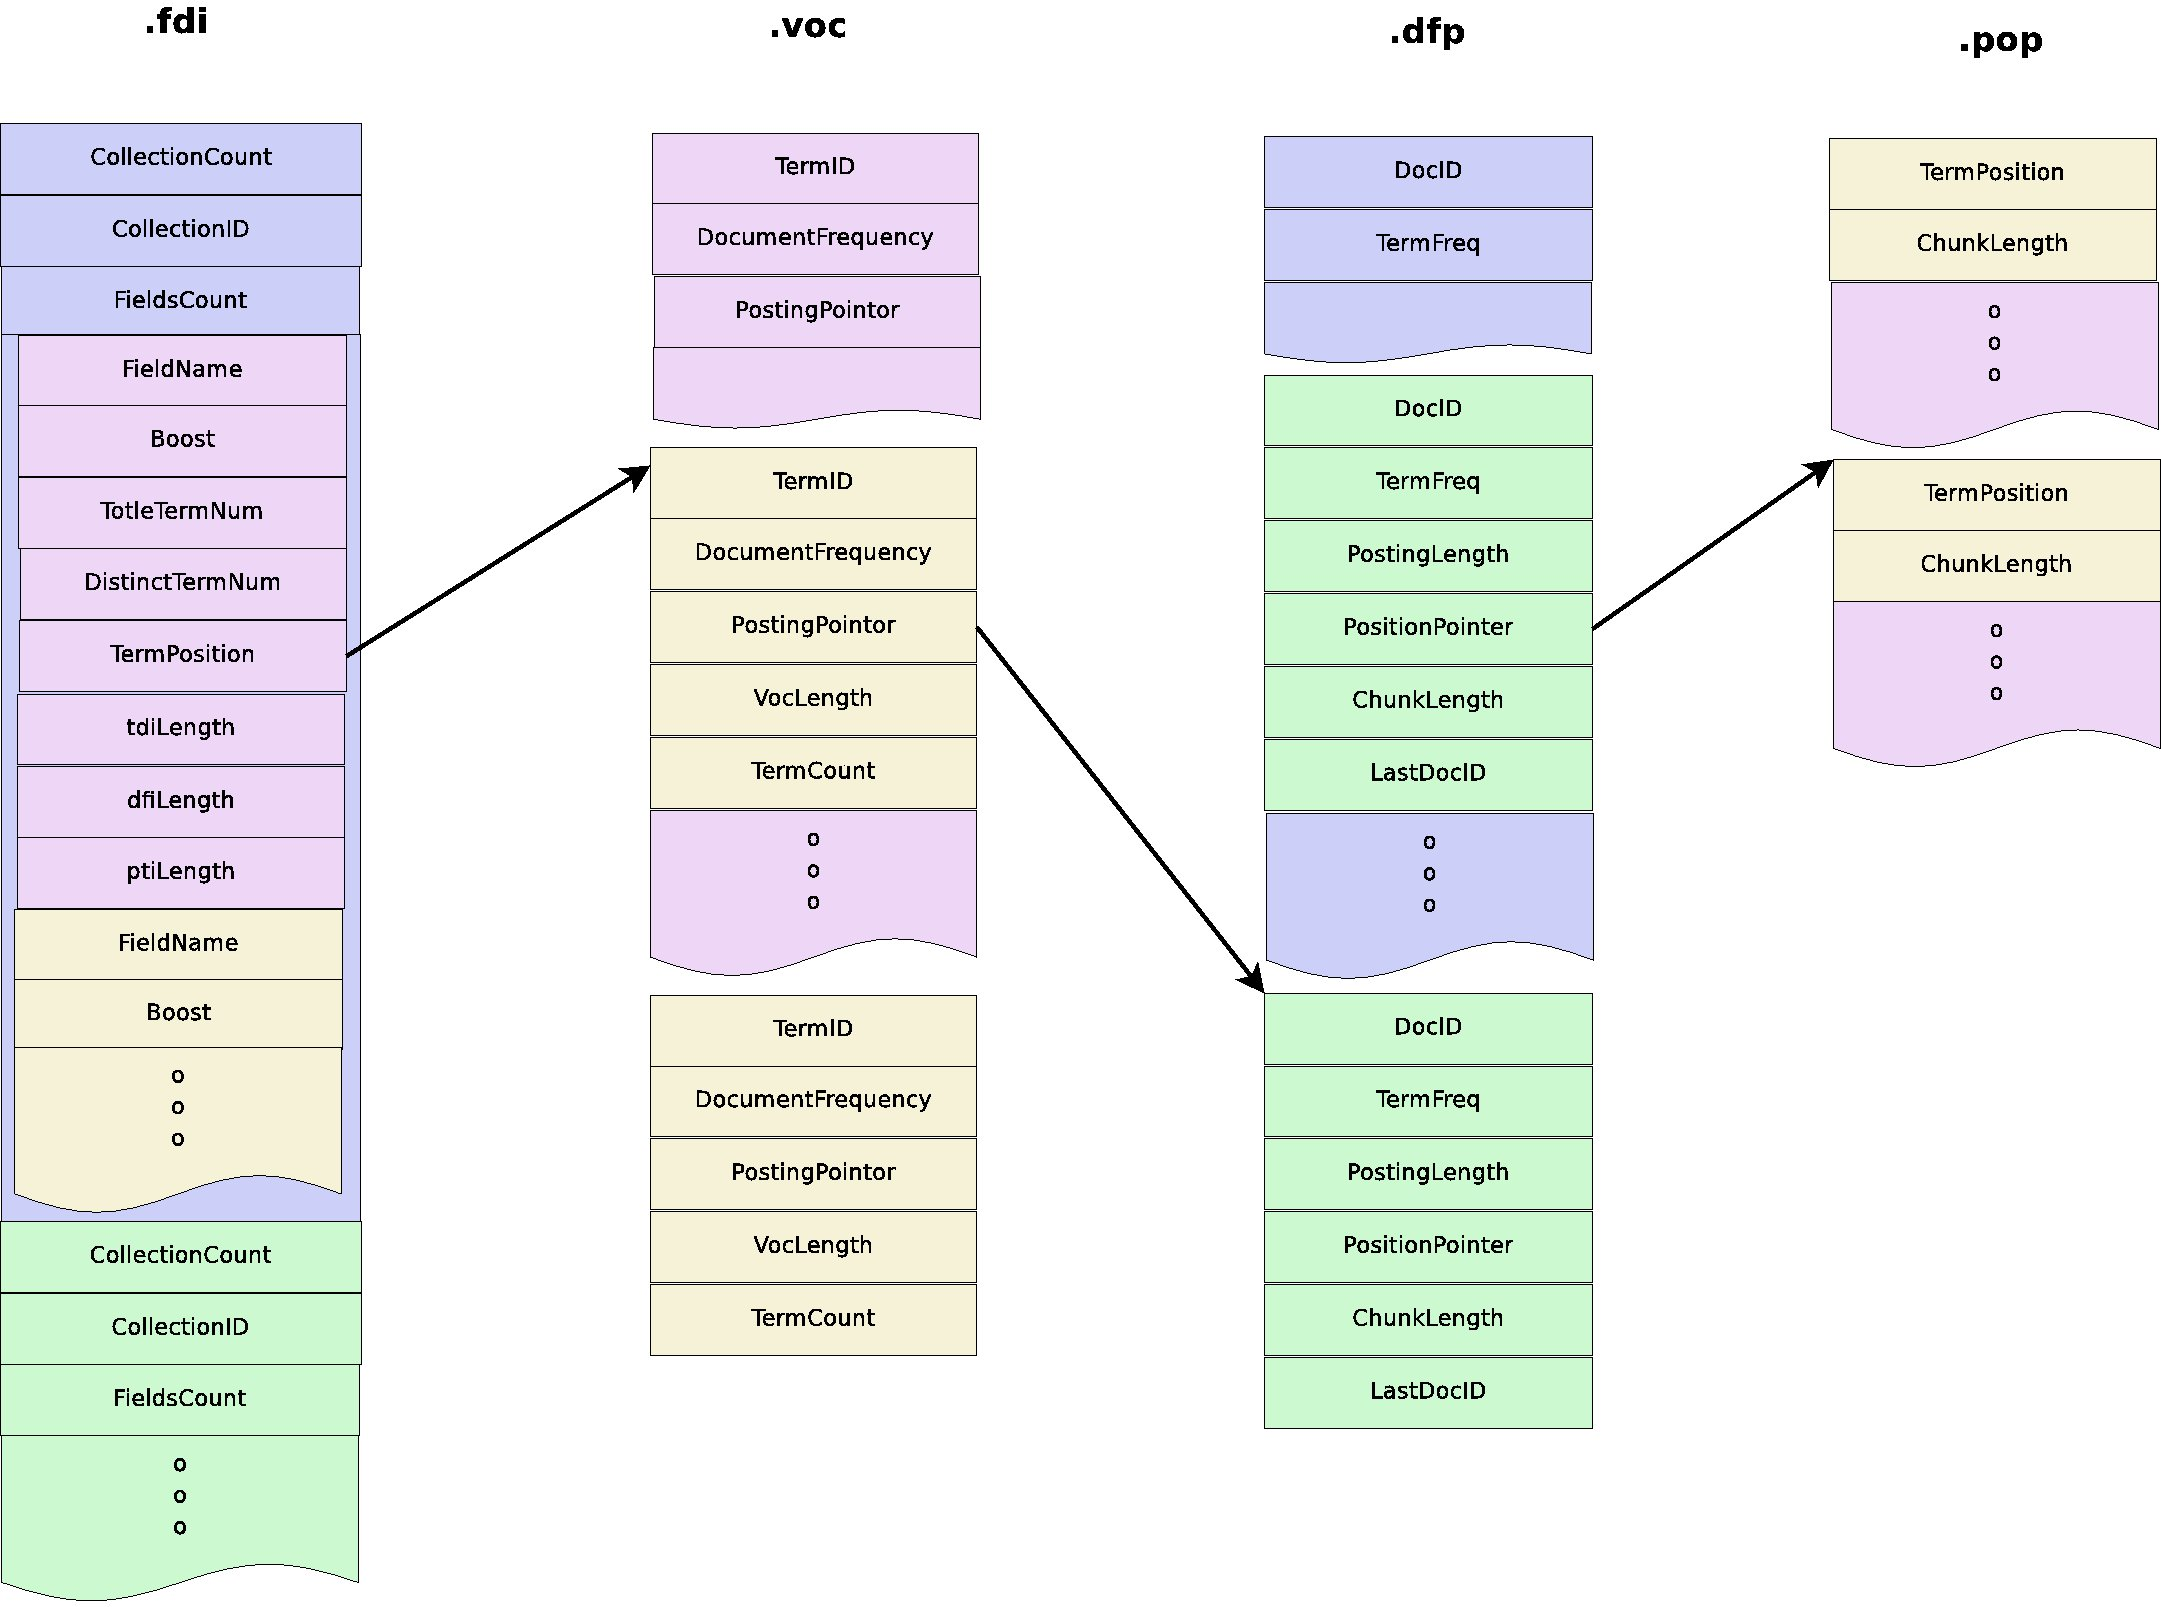
\includegraphics[width= \textwidth]{Figures/barrelFormat.jpg}}
\caption{Index format of a barrel}\label{barrelFormat}
\end{figure}
\par
Let us illustrate these files one by one.

\begin{description}
\item[.fdi] stores information of all fields.

{\scriptsize
\selectfont
\begin{tabular}{ p{.17\textwidth}|p{.06\textwidth}|p{.6\textwidth}}
\textbf{Property} & \textbf{Type} & \textbf{Description}\\
\hline

CollectionCount & Int32 & The count number of collections in this barrel\\
CollectionID & Int32 & The collection id of this collection\\
FieldsCount & Int32 & The count number of fields in this collection\\
FieldName  & string & Field name\\ 
Boost  & Byte  & Boost value of this Field\\
TotalTermNum  & Int64  & Total term number of this Field\\
DistinctTermNum  & Int64  & Total distinct term number of this Field\\
TermPosition  & Int64  & File offset of this Field's vocabulary information in the .voc file\\
tdiLength  & Int64  & Length of this Field's vocabulary information in .voc file\\
dfiLength  & Int64  & Length of this Field's document-frequency postings in the file .dfp\\
ptiLength  & Int64  & Length of this Field's position postings in the file .pop\\

\end{tabular}
}
\item[.voc] vocabulary information of all fields.

{\scriptsize
\selectfont
\begin{tabular}{ p{.17\textwidth}|p{.06\textwidth}|p{.6\textwidth}}
\textbf{Property} & \textbf{Type} & \textbf{Description}\\
\hline
TermID & Int32 & Term ID, it is stored with d-gap encoded.\\
DocumentFrequency & Int32 & The Document frequency, which means how many documents that this term has appeared.\\
PostingPointer & Int64 & File offset of this term's document-frequency posting in the .dfp file\\
VocLength  & Int64 & Same as tdiLength in .fdi\\ 
TermCount  & Int64 & Same as DistinctTermNumin .fdi\\
\end{tabular}
}

\item[.dfp] document-frequency posting.

{\scriptsize
\selectfont
\begin{tabular}{ p{.17\textwidth}|p{.06\textwidth}|p{.6\textwidth}}
\textbf{Property} & \textbf{Type} & \textbf{Description}\\
\hline
DocID               & Int32 & Document ID, which is stored with d-gap encoded.\\
TermFrep            & Vint64 & Term frequency in this document.\\
PostingLength   & Vint64 & Length of this posting\\
PositionPointer  & Vint64 & File offset of the corresponding position posting in the .pop file.\\ 
ChunkLength     & Vint64 & Same as PostingLength\\
LastDocID           & Vint32 & Last document id of this posting.\\
\end{tabular}
}

\item[.pop] position posting.The positions of a term in a document is written in the .pop file sequentially.

\end{description}
\par



\subsection{IndexMerger}

IndexMerger takes charge of merging multiple index barrels if the merge conditions are satisfied. When a merge event happens, all the barrels that are needed to be merged are ordered according to the document number that each barrel has contained, then the merging process will be proceeded field by field. FieldMerger is responsible for merging same field of a collection in different barrels, and PostingMerger will merge postings at the term level.

\begin{figure}[htb]
\centerline{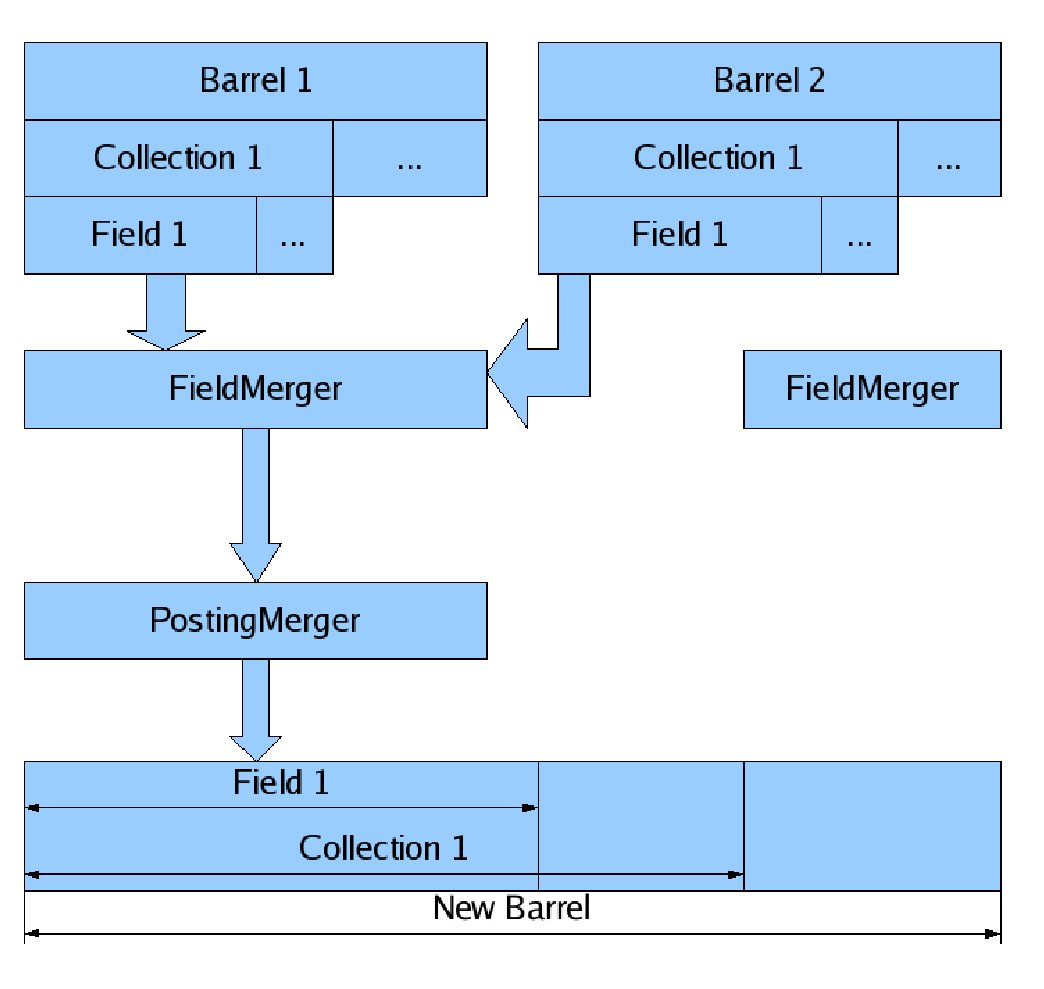
\includegraphics[width=0.4\textwidth]{Figures/indexmanager.jpg}}
\caption{Hierarchy of IndexMerger}\label{indexmanager}
\end{figure}

IndexMerger could be configured to run within a stand-alone thread, in that case, there exist complicated index sychronization mechanism between IndexMerger and IndexReader, because IndexMerger will remove old index barrels after a successful merge, while the IndexReader can not always check the validation due to the performance of searching.


\subsection{IndexReader}


\begin{figure}[h!]
\centerline{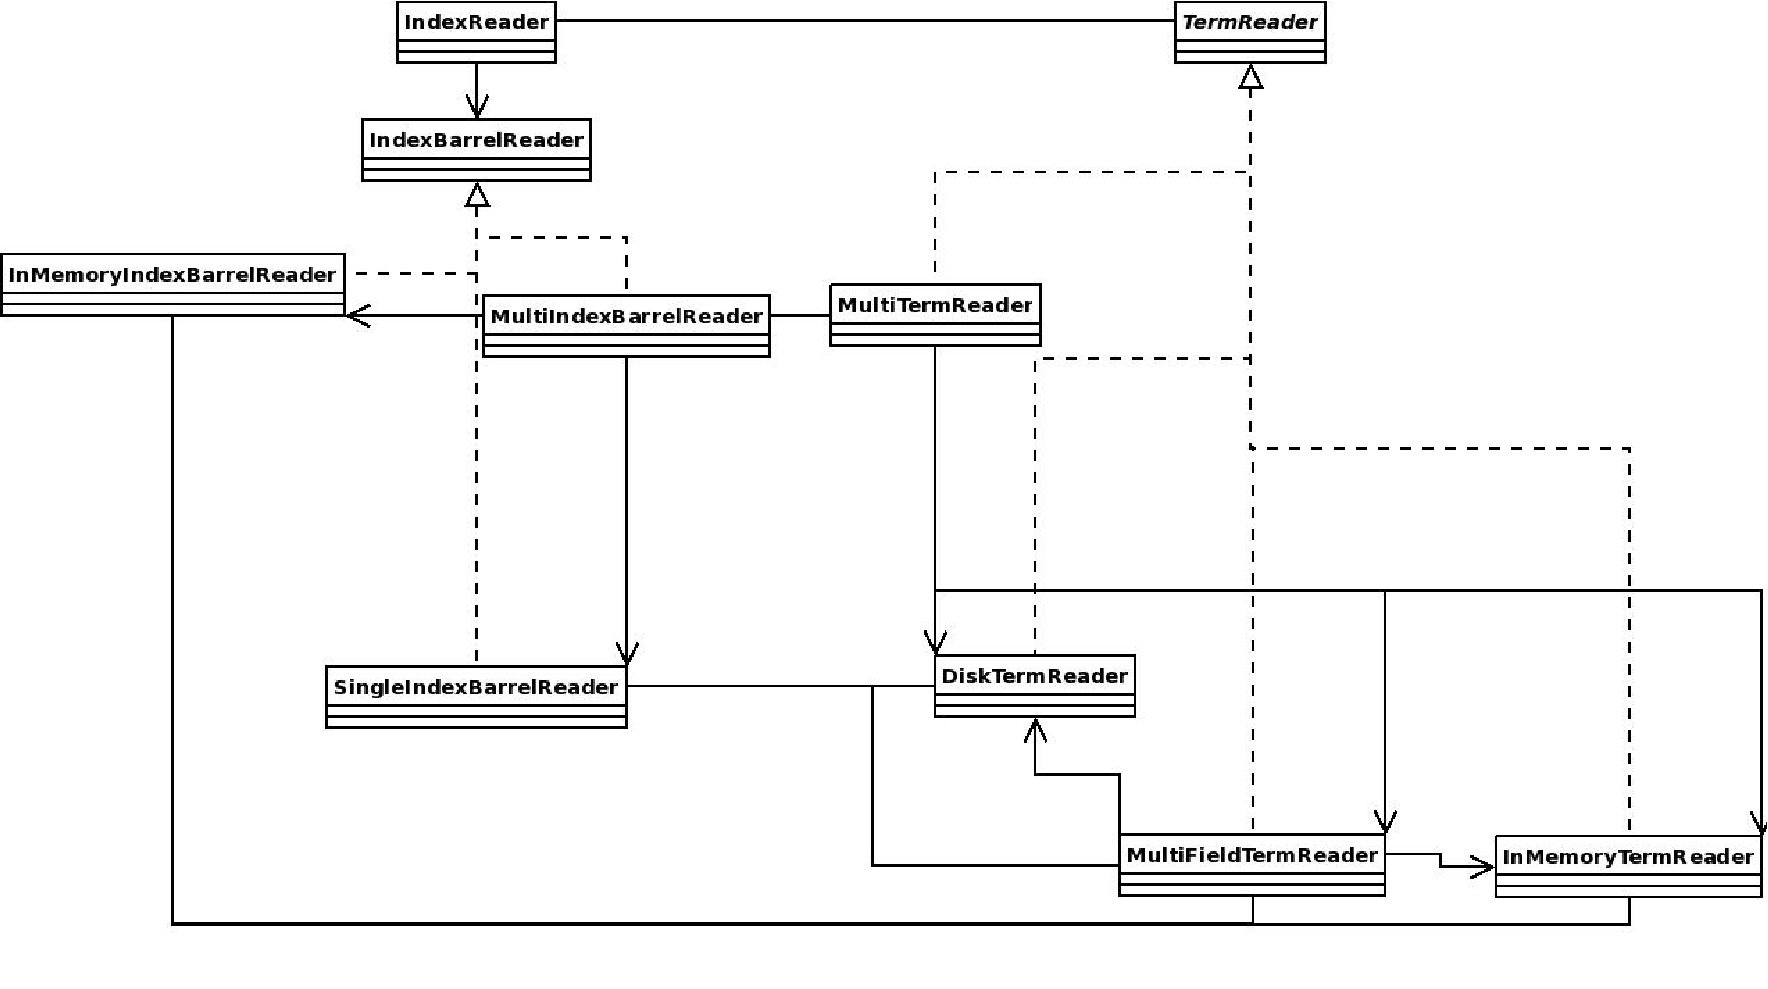
\includegraphics[width=\textwidth]{Figures/indexreader.jpg}}
\caption{Components of IndexReader}\label{indexReader}
\end{figure}


\par
IndexReader is the interface to read inverted indexes and search them. Figure \ref{indexReader} gives a detailed class diagram of the components of IndexReader. When IndexReader is created, it will open the index barrels and return an instance of TermReader to users. TermReader takes charge of seeking a term in the vocabulary of the indexes, and then iterating its corresponding posting list according to the user's requests. SingleIndexBarrelReader is used to open a single index barrel and return its TermReader, here it is the DiskTermReader. Because IndexManager should support on-line indexing, which means the indexes could be searched during index construction, therefore, those indexes that have not been flushed to disk should also allow being searched, InMemoryIndexBarrelReader takes this responsibility. What's more, since there may exist several barrels in the system, then we have MultiIndexBarrelReader which contains several instances of SingleIndexBarrelReader or InMemoryIndexBarrelReader, each of which 
takes charge of reading their corresponding sub-index. Accordingly,  the TermReader got by InMemoryIndexBarrelReader should be InMemoryTermReader, and the TermReader got from MultiIndexBarrelReader should be MultiTermReader, which is composed of several instances of DiskTermReader and InMemoryReader similarly.

\par
After getting an instance of TermReader, the user could use it to search the inverted indexes: if the term to be queried could be found by TermReader in the indexes, then TermReader could return an index iterator TermDocFreqs or TermPositions. Just as Figure \ref{indexmanager} shows. TermDocFreqs will iterate the document-frequent postings and TermPositions will iterate document-frequent postings and position postings both, therefore TermPositions is inherited from TermDocFreqs. They are the major search utilities interface classes exposed to users.\par

\begin{figure}[h!]
\centerline{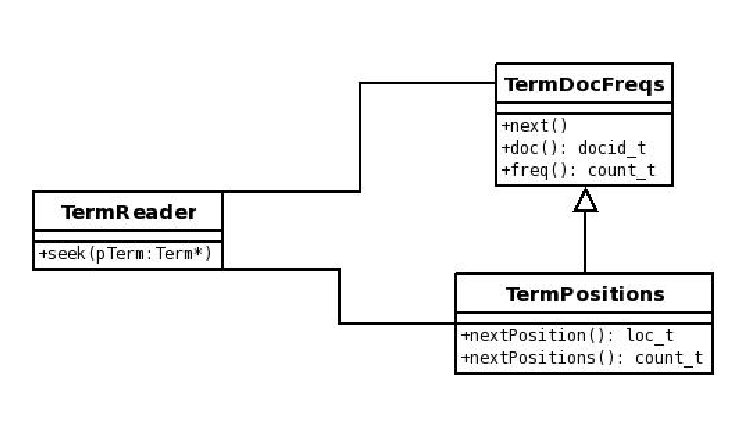
\includegraphics[width=0.5\textwidth]{Figures/termPos.jpg}}
\caption{TermDocFreqs and TermPositions}\label{termPos}
\end{figure}


\subsection{Search Optimization}
Search performance is always the most important design issue for index design. We have two approaches for search optimization:

\subsubsection{Embedded Skiplist}
Embedded skip list is used to accelerate conjunction operation of multiple posting lists. Suppose we have two postings that contain doc ids:
\begin{lstlisting}[language=C]
1,2,3,4,10,11,100,120,1000,...

1,10,1000,...
\end{lstlisting}
The conjunction operation for these two postings should be: $1,10,1000,...$ . For index without embedded skiplist, we must read and decompress all posting data, while if we have implemented skiplist within posting list,
we could use these operations to avoid of frequent disk IO:
\begin{lstlisting}[language=C]
  pDocIterator->skip(10);
  pDocIterator->skip(1000);
\end{lstlisting}

The assumptions for the embedded skiplist are:
\begin{itemize}
 \item Seeking forward to a certain place will take less time than read. In the above example: it means within the first posting, the time taken by the file seek operation from doc id of 1 to doc id of 10, is less than the time 
taken by reading all posting data between those two doc ids.  This is especially true for conjunction operation over short posting list and long posting list.
 \item Document ids within each posting list should be an incremental order. 
\end{itemize}

Figure \ref{skiplist} shows the detailed design for an embedded skiplist---For simplicity, it has not contained the information of term position posting lists:
\begin{figure}[h!]
\centerline{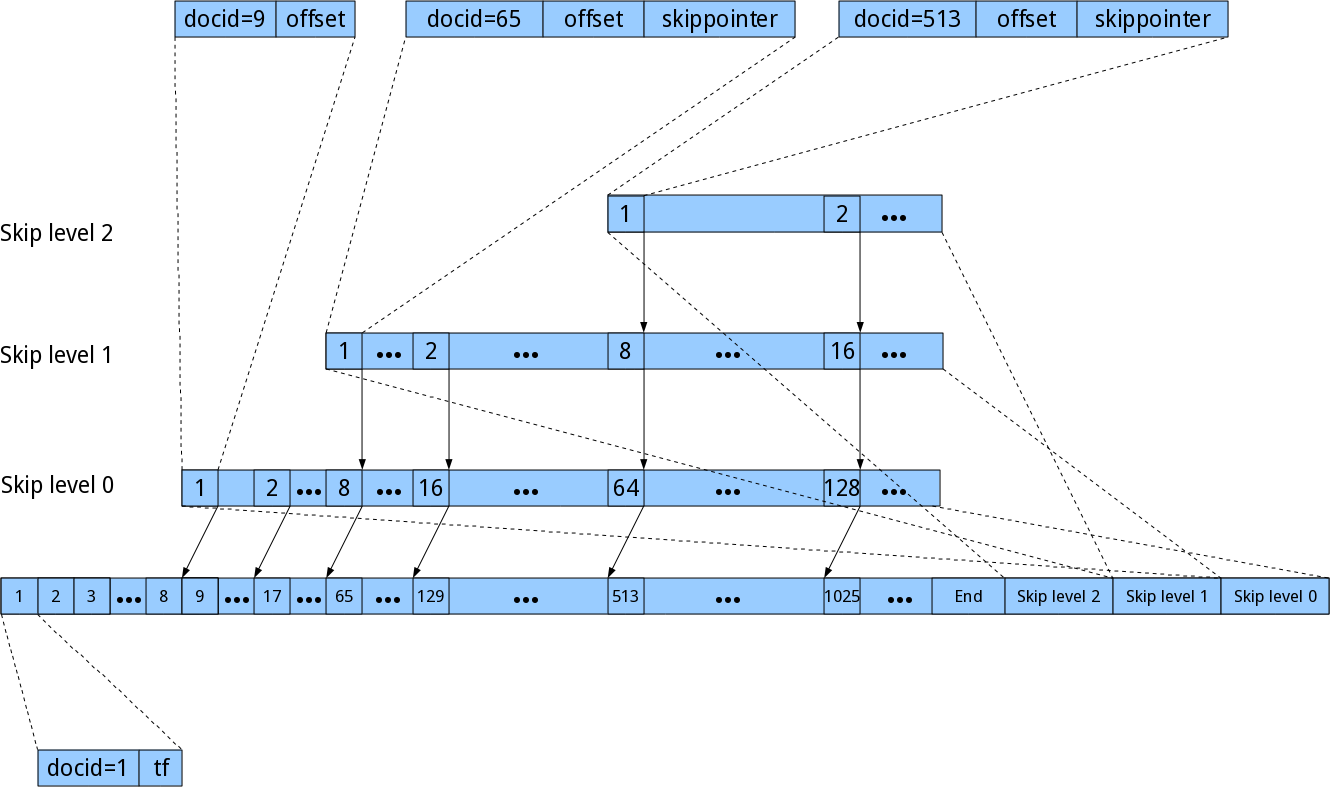
\includegraphics[width=0.8\textwidth]{Figures/skip.png}}
\caption{Embeded SkipList Design}\label{skiplist}
\end{figure}

Several points are needed to be illustrated:
\begin{itemize}
 \item In this example, we have embedded a skiplist with an interval of 8 and a max skip level of 3. Which means, during indexing, we will record a skip point every 8 documents. The skip interval of the second skip level is $8*8=64$,
while the skip interval of the upmost skip level is $8*8*8=512$.
 \item Each skip point contains two kinds of data:
   \begin{enumerate}
    \item Current skipped document id.
    \item File offsets of skipped point, including both \texttt{dfp} posting list and \texttt{pos} posting list.
   \end{enumerate}
 \item We should consider the location of skiplist data. In the example graph, the skiplist data locates at the end of each posting. It is very convenient for posting merging, because skiplist data will not be generated until the overall posting
list is merged, if we put skiplist data at the end of each posting, we could directly write skip data just after merging postings.  However, such design will hurt the query performance---it will lead to file seek operations not sequential
any more. Therefore, with the eventual implementation, the skiplist data is put at the head of each posting---In this case, it's pretty inconvenient for posting merge operation, we will discuss this issue in the following part.
\end{itemize}

Figure \ref{skiplist-merge} illustrates the design issue for posting merge when we have added embedded skiplist data to index. From the upper part of this graph we can see the posting merge is pretty direct, while if we put skiplist data
at the beginning of the posting list, it will introduce more complicated design: During merging operation, we could directly write the skiplist data of merged posting to the index file, while we need an extra intermediate file to store the 
merged posting data. After all posting merging is finished, we should copy data from that intermediate file to index file. Only through this operation could we provide skip list data at the beginning of each posting.

\begin{figure}[h!]
\centerline{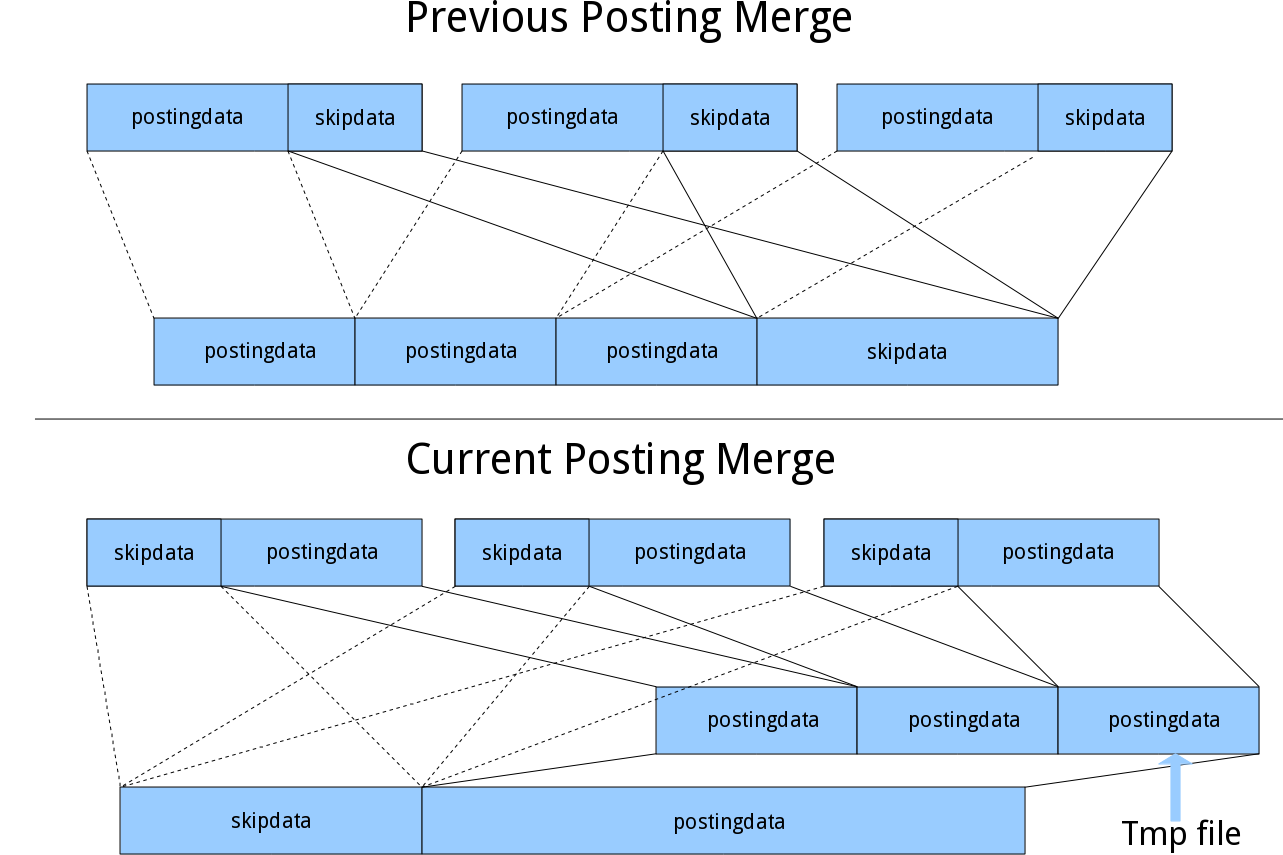
\includegraphics[width=.8\textwidth]{Figures/skipmerge.png}}
\caption{Posting Merge With SkipList}\label{skiplist-merge}
\end{figure}


Another design issue for skiplist design is also caused by the posting merge, seen from figure \ref{skiplist-interval}:
\begin{figure}[h!]
\centerline{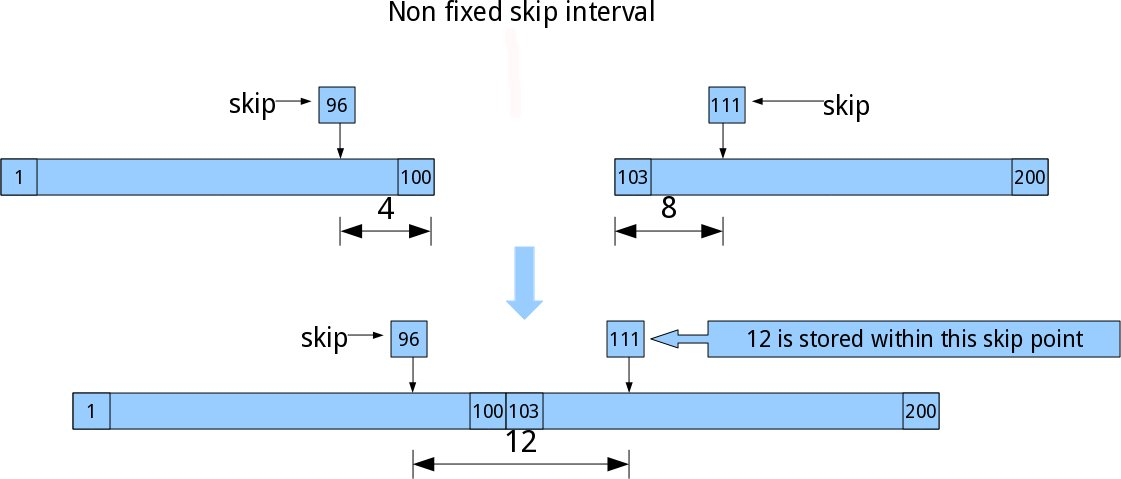
\includegraphics[width=.8\textwidth]{Figures/skipinterval.jpg}}
\caption{Unfixed Skip Interval Design}\label{skiplist-interval}
\end{figure}

In this example, both two posting have a skip interval of 8. However, at the end of the first posting, there are only 4 documents left, as a result, after merging these two postings, the skip interval between document $96$ and
document $111$ should have to be reconsidered:
\begin{itemize}
 \item One solution is to still keep the fixed skip interval. In this case, all skip data will have to be regenerated after posting merging.
 \item The other solution is to introduce unfixed skip interval. In this case, the skipinterval between document $96$ and document $111$ will be 12 instead of 8 any more.
\end{itemize}

IndexManager adoptes the second solution, because it requres less operation for merging skiplist data. Obviously, it introduce extra storage overheads because we have to record skip interval value for certain skip points.

\subsubsection{New Compression}
New compression is another approach for search optimization. Due to the fact that all of the cutting-edge compression schemes are totally different with general variable byte length based solution, IndexManager must provide a 
good abstraction so that all kinds of index format can be supported and switched easily just by a configuration parameter. Shown in figure \ref{newindexclass}, the basic abstraction is \texttt{PostingWriter} and \texttt{PostingReader}.
They are two interface classes owned by IndexWriter and IndexReader. We provide new compression based index within \texttt{EPostingWriter} and \texttt{EPostingReader}.

\begin{figure}[h!]
\centerline{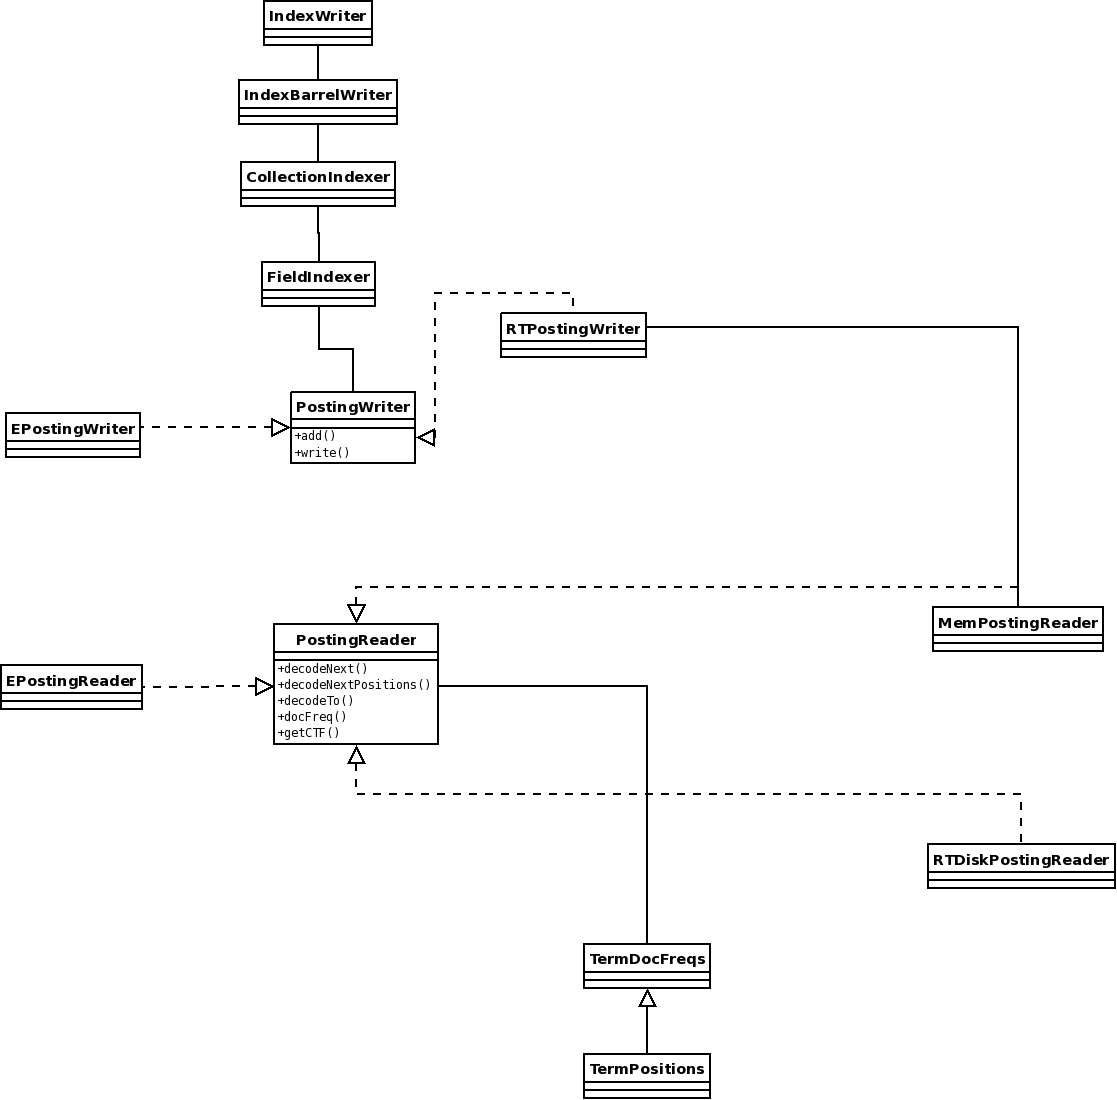
\includegraphics[width=.8\textwidth]{Figures/newindexclass.png}}
\caption{Class Diagram Overview For New Index}\label{newindexclass}
\end{figure}


In order to be flexible enough to switch among all the new compression schemes, IndexManager provides a wrapper class:

\begin{lstlisting}[language=C]
template<typename PrimaryCompressor>
struct CompressorType
{
    int compress(uint32_t* input, uint32_t* output, int num_input_elements) const;

    int decompress(uint32_t* input, uint32_t* output, int num_input_elements) const;
};
\end{lstlisting}

So that if we want to change the compression scheme, we just need to redefine cooresponding template parameters:

\begin{lstlisting}[language=C]
typedef CompressorType<PForDeltaMix_Compressor> DocIDCompressor;

typedef CompressorType<S16_Compressor> TermFreqCompressor;

typedef CompressorType<S16_Compressor> TermPosCompressor;
\end{lstlisting}


Before illustrating how the new compression schemes are used within index, let us first describe how those compression approaches work at first:
\begin{enumerate}
 \item Variable-Byte Coding: Variable-byte compression represents an integer in a variable number of bytes, where each byte consists of one
status bit, indicating whether another byte follows the current one, followed by 7 data bits. Variable-byte compression does not achieve a very
good compression ratio, but is simple and alows for fast decoding, as a result, it is the most popular compression solution in existing IR frameworks.
 \item S9: Simple9 coding is an algorithm proposed in \cite{anh2005inverted} that combines good compression and high decompression speed. The basic
idea is to try to pack as many values as possible into a 32-bit word. This is done by dividing each word into 4 status bits and 28 data bits, where the
data bits can be partitioned in 9 different ways. For example, if the next 7 values are all less than 16, then we can store them as 7 4-bit values. Or
if the next 3 values are less than 512, we can store them as 3 9-bit values(leaving one data bit unused).

Simple9 uses 9 ways to divide up the 28 data bits: 28 1-bit numbers, 14 2-bit numbers, 9 3-bit numbers(one bit unused), 7 4-bit numbers, 5 5-bit numbers
(three bits unused), 4 7-bit numbers, 3 9-bit numbers(one bit unused), 2 14-bit numbers, or 1 28-bit numbers. The 4 status bits store which of the 9 cases
is used. Decompression can be optimized by hardcoding each of the 9 cases using fixed bit masks, and using a switch operation on the status bits to select the case.
 \item S16: Simple16 \cite{zhang2008performance} uses the same basic idea as S9, but has 16 ways of partitioning the data bits, where each of the 16 cases uses 
all of the 28 data bits. The result is that S16 approximately matches the speed of S9, while achieving slightly better compression. 
 \item PForDelta: This is a compression method recently proposed in \cite{zukowski2006ssr} that supports extremely fast decompression while also 
achieving a small compressed size.  PForDelta first determines a value $b$ such that most of the values to be encoded(say, $90\%$) are less than $2^b$ and thus
fit into a fixed bit field of $b$ bits each. The remaining values, called $exceptions$, are coded separatedly.  If we apply PForDelta to blocks containing some multiple
of 32 values, and finally patching the result by decoding a smaller number of exceptions. This process can be implemented extremely efficiently by providing,
for each value of $b$, an optimized method for extracting 32 b-bit values from $b$ memory words. PForDelta can be modified and tuned in various ways by choosing
different thresholds for the number of exceptions allowed, and by encoding the exceptions in different ways.

Within IndexManager, the composite compression scheme that uses variable-byte approach to compress the exceptions is names as \texttt{PForDeltaMix} compressor.
From the research work in \cite{yan2009compressing}, another improvements for PForDelta have been presented: Recall that the implementations of PForDelta 
in previous work encode a block of 128 value by first allocating 128 b-bit slots, and then for those $90\%$ of the values less than 2b directly storing them in their 
corresponding slots. For each value larger than 2b , called a exception, we store an offset value in the exception's corresponding slot indicating the distance from 
the current exception to the next one, and the actual value of the exception in some additional space after the 128 b-bit slots. One disadvantage of such a code 
structure is that when two consecutive exceptions have a distance of more than 2b , we have to use more than one offset to represent the distance, by forcing 
additional exceptions in between these two exceptions. We cannot solve this problem by simply increasing b since this would waste lots of bits on $90\%$ of values; 
but if we decrease b more exceptions will be produced. This means in particular that this version of PForDelta cannot profitably use any values of b less than b = 3.
To overcome this problem, they present a new code structure for PForDelta that stores the offset values and parts of the exceptions in two additional arrays. 
In particular, for an exception, they store its lower b bits, instead of the offset to the next exception, in its corresponding b-bit slot, while they store the higher overflow
bits and the offset in two separate arrays.  These two arrays can be further compressed by any compression method, and they find that S16 is particularly suitable for
this. Another improvement is in the selection of the b value for each block. As it turns out, selecting a constant threshold for the number of exceptions does not 
give the best tradeoff between size and speed. Instead, they model the selection of the b for each block as an optimization problem: initially assign the b with the
smallest compressed size to each block, and then increase speed as desired by selecting a block that gives us the most time savings per increase in size, and change the b 
of that block. For a given target speed, we can easily derive simple global rules about the choice of b, instead of running the iterative optimization the above. Thus this 
version can be very efficiently implemented even on very large collections.

\par
Within IndexManager, we call this composite compression scheme PForDelta-Mix-S16 compressor. According to the description above, the optimization procedure for choosing
best b value takes longer time---around 10 times longer than general PForDelta according to the experiments, while it can achieve more benefits during search operations. 
\end{enumerate}

Based on the above template wrapper for compressor, as well as a suit of compression schemes, such as: S16, PForDelta, PForDeltaMix, PForDeltaMixS16, ..., etc, we provide
two kinds of index format within which any of the new compression scheme could be applied, shown in figure \ref{newindex}:

\begin{figure}[h!]
\centerline{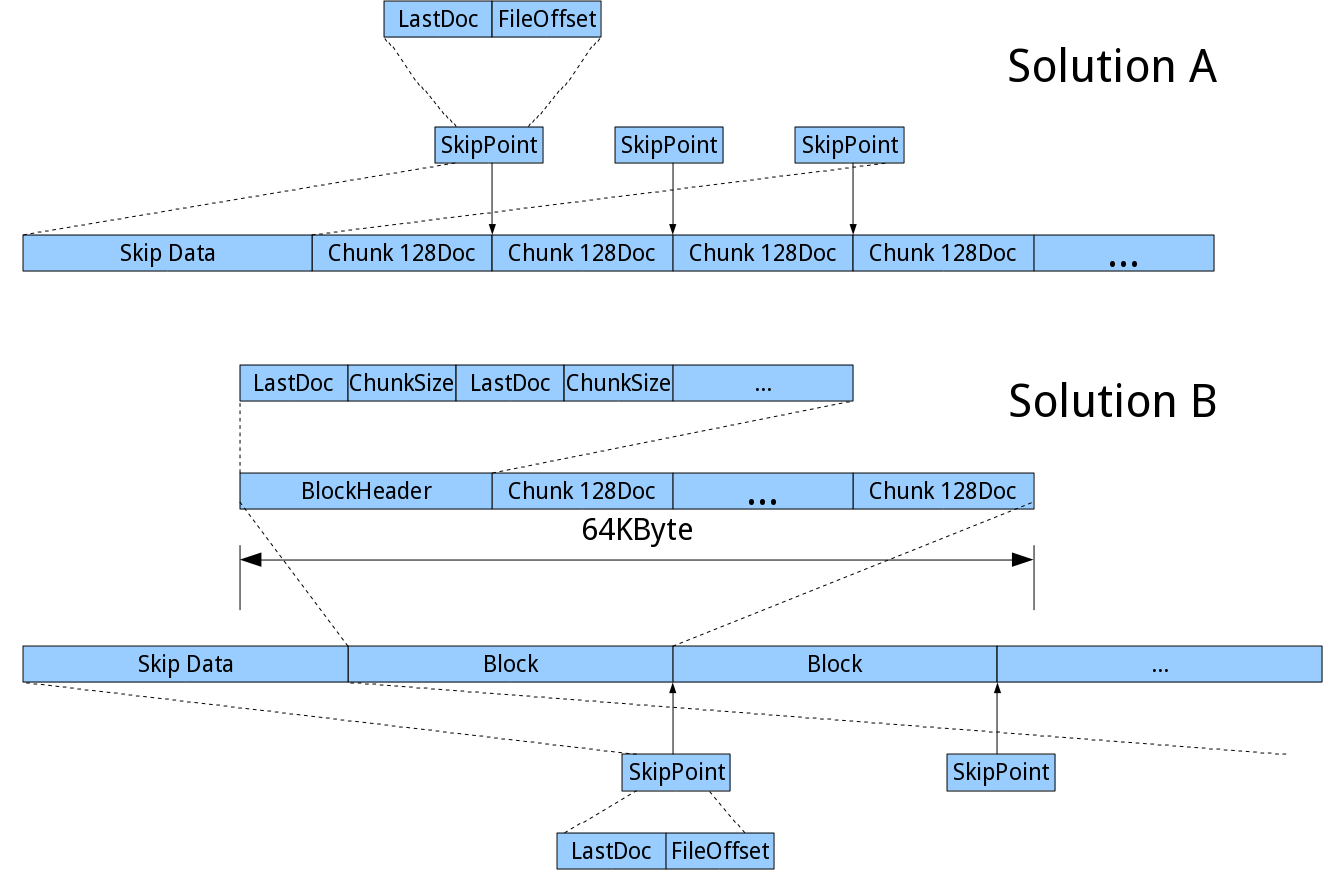
\includegraphics[width=.8\textwidth]{Figures/newindex.png}}
\caption{Chunk and Block Type Index}\label{newindex}
\end{figure}

\begin{itemize}
 \item \texttt{Chunk Type}---solution A in figure \ref{newindex}\par
Chunk type index directly compress posting data for every 128 documents, and we call each compression unit with the terminology $chunk$. The embedded skiplist data is totally 
the same with the original index, with a fixed skip interval of 128.

 \item \texttt{Block Type}---solution B in figure \ref{newindex} \par
The idea of block type index comes from the requirements that disk IO performs the best for a fixed block of size. In this design, the posting data is partitioned into a series of
block each of which has a fixed size, say, 64K bytes. Within each block, there are a series of chunk that contains posting data for every 128 documents. There are several
benefits for block type index over chunk type:
\begin{enumerate}
 \item It is very easy to provide posting level cache based on block type index. \par
Given a large scale web search system, we need to set up multi level cache mechanism to support huge search requests. Posting level cache is always the lowest level and the most
difficult to design. However, having block type index, implementing such cache is much easier: we just need to record each block identifier and store them into cache.
 \item We could provide more compression to posting data: \par
When implementing chunk type index, besides the chunk that contains posting data for every 128 documents, we still need to store these values to posting list:
\begin{itemize}
 \item Size of each chunk. Generally, it is stored using variable byte compression.
 \item Skip data, containing current skip doc id and file offsets. They are also stored using variable byte compression.
\end{itemize}
With block type index, we only need to set up an embedded skip list for blocks, while within each block, we have block header data that contains size and last doc id for each chunk,
these data are put together so we could use another better compressor to compress block header data.

The weakness for block type index is also remarkable: It supposes each posting list would occupy at least one block. For smaller corpus, most of the index contains useless data.
So block type index is more suitable to serve as extremely large index, especially for supporting web search, while chunk type index is more general.  
\end{enumerate}
 
\end{itemize}


There are two more design issues caused by the new compression scheme:
\begin{itemize}
 \item Location of term position posting data. \par
Just the as the original variable byte length based index, the term position posting data is still put into another file, instead of putting together with doc ids and term frequencies, shown
in figure \ref{termpos-chunk};

\begin{figure}[h!]
\centerline{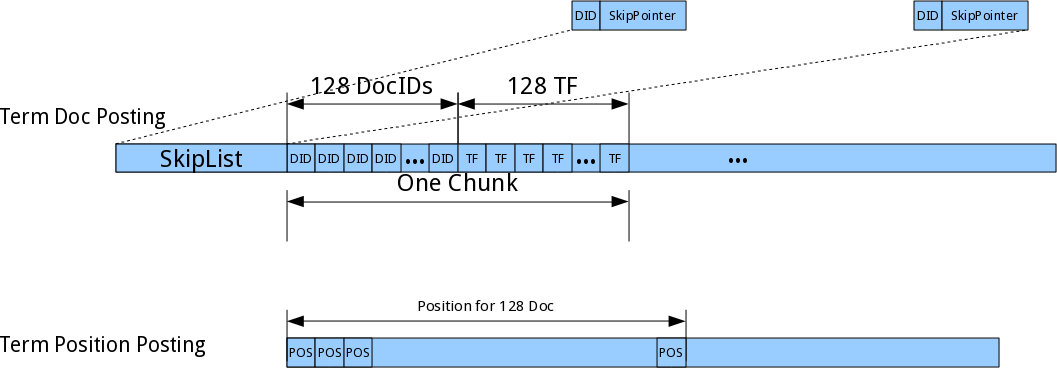
\includegraphics[width=.8\textwidth]{Figures/termpos.png}}
\caption{Term Position Data for Chunk Type Index}\label{termpos-chunk}
\end{figure}

We design in this way just for better reusage for existing IndexManager components.
 \item Posting merge issue. \par
Another design issue is caused by posting merge. No matter chunk type or block type index, all of them compress posting data in a batch way with fixed documents. When merging two 
postings, suppose the last chunk for the first posting only contains posting data for 21 documents, we can only have two choices to deal with such kinds of data chunk:
\begin{enumerate}
 \item Decompress all posting data of the second posting, then recompress them together with the data from the first posting.
 \item For every chunk, do not compress data from a fixed size of documents.
\end{enumerate}
IndexManager has adopted the first choice, because the other approach has introduced more overheads---it will cause the inefficiency of PForDelta based compression scheme. 
As a result, given that either of chunk type or block type index is adopted, we should have a much slower merging performance, both of these two kinds of index should be chosen according
to practical situations.
\end{itemize}


\chapter{Succinct Self-Index}
\lhead{Chapter 4. \emph{Succinct Self-Index}} % this is for the header on each page - perhaps a shortened title

As performance of inverted list based search engine is limited by disk I/O, we build a in-memory one to provide much higher throughput based on the family of
succinct data structures. Most available solutions for succinct in-memory index can be classified into two categories: compressed suffix array(CSA) and FM-index.
Both use wavelet trees to store data and support three basic operations: \(access\), \(rank\) and \(select\). Our solution is based on FM-index and document array. It
trades long build time and large memory consumption for low latency and high concurrency.


\section{One Cache-miss Bitvector}

A wide variety of succinct data structures are build upon wavelet trees, each node of which is a bitvector (or integer vector for multi-ary wavelet trees). The three bitvector
operations --- access, rank and select --- are fundamental for algorithms on wavelet trees. Figure \ref{fig:rankselect} shows the definition of a rank/select operation
on a basic bitvector. Thus a carefully designed bitvector with good performance is crucial for a fast succinct index solution. In our implementation major part of computation
occurs on document array. To maximize the performance of retrieval algorithms, we designed one cache-miss bitvector for document array.

\begin{figure}[h!]
\centerline{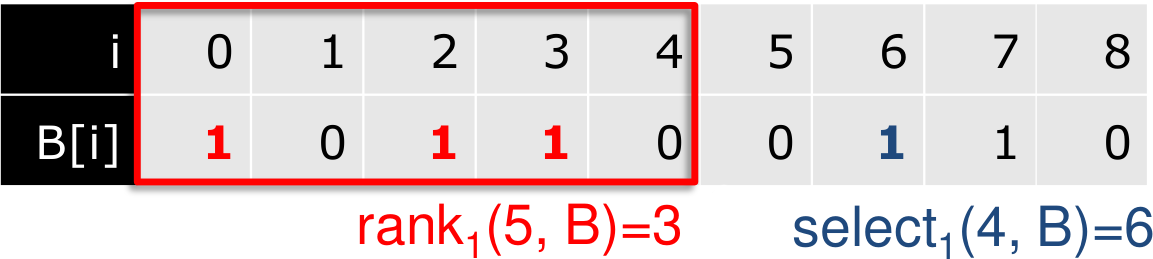
\includegraphics[width=0.6\textwidth]{Figures/rankselect.png}}
\caption{Rank/Select Operation of a Bitvector}\label{fig:rankselect}
\end{figure}


\subsection{Data Structure}
The design of bitvector with rank/select operation supported is to struggle with cache misses, during a retrieval process over wavelet trees, there are intensive rank operations
getting involved, as a result, the number of cache misses is one of major bottleneck for performance improvements since the complexity of wavelet trees is optimal. A general
design of bitvector will introduce 4-6 cache misses for each rank operation, and there are several research works to reach state-of-the-art results on reducing cache misses,
such as \cite{gog2013optimized}, \cite{zhou2013space}, which claimed to have 2 to 3 cache misses for each rank operation, see in figure \ref{fig:cachemisses}.

\begin{figure}[h!]
\centerline{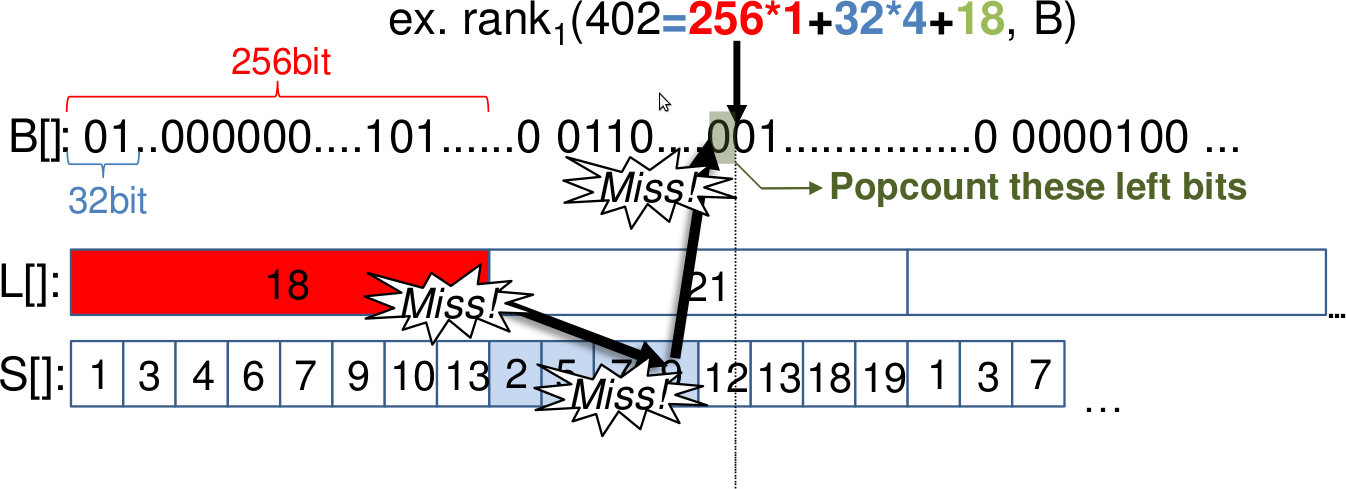
\includegraphics[width=0.6\textwidth]{Figures/cachemisses.png}}
\caption{3 Cache/TLB Misses Per Rank of a Bitvector}\label{fig:cachemisses}
\end{figure}


Our solution is to split the original data into blocks of 384 bits (uint64\_t[6]), then for each block we store the rank value for its initial position and the partial rank values of each 64-bit integer. The partial rank values are stored like this: each partial value is not more than 384 (9 bits), and each block has 7 partial values, so we need at least \(9*7=63\) bits which can be compacted into a 64-bit integer. Thus each block is exactly 512 bits. Answering a rank() query, we calculate the block index and offset, and sum up the initial rank of that block, the partial rank of one particular integer and the popcount of part of that integer, all of which reside in a single cache line inferring exact one cache miss.

The structure of a super block looks like below:
\begin{lstlisting}
struct SuperBlock
{
    uint64_t rank_;
    uint64_t subrank_;
    uint64_t bits_[6];
};
\end{lstlisting}

\subsection{Rank Query}

It is convenient to calculate \(rank\) value on one cache-miss bitvector. First we calculate the superblock and block indexes for queried position. Then the \(rank\) value is
\begin{align*}
  rank_1(pos) &= sb[sb\_index(pos)].rank\_ \\
              &+ (sb[sb\_index(pos)].subrank\_ >> (9 * b\_index(pos)) | 511) \\
              &+ popcount(mask(sb[sb\_index(pos)].bits\_[b\_index(pos)], b\_offset(pos)))
\end{align*}

\section{Wavelet tree}

The Wavelet Tree is a succinct data structure to store strings in compressed space. Wavelet Tree converts a string into a balanced binary-tree of bit vectors, where a 0 replaces half of the symbols, and a 1 replaces the other half. This creates ambiguity, but at each level this alphabet is filtered and re-encoded, so the ambiguity lessens, until there is no ambiguity at all.
The tree is defined recursively as follows:

\ \ \ \ 1. Take the alphabet of the string, and encode the first half as 0, the second half as 1, for example, {a,b,c,d} would become {0,0,1,1};

\ \ \ \ 2. Group each 0-encoded symbol, {a,b}, as a sub-tree;

\ \ \ \ 3. Group each 1-encoded symbol, {c,d}, as a sub-tree;

\ \ \ \ 4. Reapply this to each subtree recursively until there is only one or two symbols left (when a 0 or 1 can only mean one thing).

For the string \('Peter Piper picked a peck of pickled peppers'\) (spaces and a string terminator have been represented as \_ and \$ respectively, due to convention in the literature) the Wavelet Tree would look like this in Table \ref{ex:awt}. Note that the strings aren’t actually stored, but are shown here for convenience.

\begin{table}[!htp]
  \caption{A Wavelet Tree}
  \label{ex:awt}
  \begin{center}
    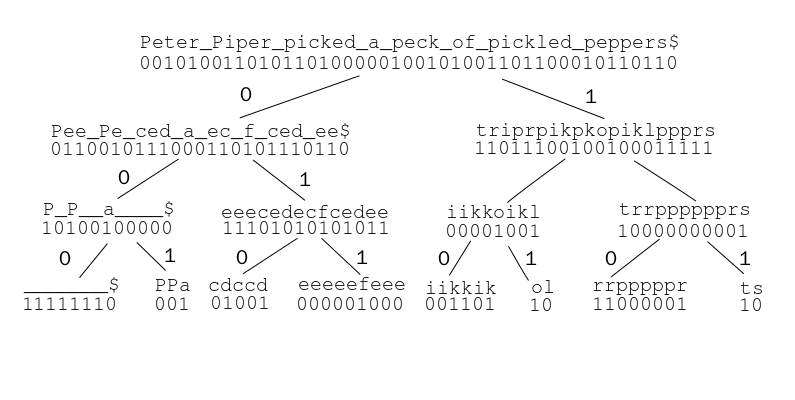
\includegraphics[width=1\textwidth]{Figures/graph1.png}
  \end{center}
\end{table}

It has the alphabet \(\{\$,P,_,a,c,d,e,f,i,k,l,o,p,r,s,t\}\), which would be mapped to \(\{0,0,0,0,0,0,0,0,1,1,1,1,1,1,1,1\}\). So, for example, \$ would map to 0, and r would map to 1.

The left subtree is created by taking just the 0-encoded symbols \(\{\$,P,_,a,c,d,e,f\}\) and then re-encoding them by dividing this new alphabet: \(\{0,0,0,0,1,1,1,1\}\). Note that on the first level an e would be encoded as a 0, but now it is encoded as a 1 (it becomes a 0 again at a leaf node).

In fact, since it is a balanced tree, we can concatenate each of the levels and store it as one single bit vector.
Actually, the data structure we used is a variant of Wavelet Tree named Wavelet Matrix, which introduced by (Claude el at,. 2012 \cite{claude2012}).
The idea of the Wavelet Matrix is to break the assumption that the children of a node v at interval \([s,e]\), must be aligned to it and occupy the same interval in the next level. Freeing the structure from this unnecessary assumption allows us to design a much simpler mapping mechanism from one level to the next: all the 0s of the level go left, and all the 1s go right. For each level, we will store a single integer \(z[l]\) that tells the number of 0s in level \(l\).

\subsection{Rank in Wavelet Tree}

A rank query is the count of 1-bits up to a specified position. Rank queries over larger alphabets are analogous – instead of a 1, it may be any other symbol.
After the tree is constructed, a rank query can be done with \(O(logA)\) (A is alphabet size) binary rank queries on the bit vectors in \(O(1)\)(Claude et al., 2008 \cite{claude2008}). The encoding at each internal node may be ambiguous, but of course it isn’t useless – we use the ambiguous encoding to guide us to the appropriate sub-tree, and keep doing so until we have our answer.

For example in Table \ref{ex:riwt}, if we wanted to know \(rank(5,e)\), we use the following procedure which is illustrated below. We know that \(e\) is encoded as 0 at this level, so we take the binary rank query of 0 at position 5. Which is 4, which we then use to indicate where to rank in the 0-child: the 4th bit (or the bit at position 3, due to 0-basing). We know to query the 0-child, since that is what e was encoded as at the parent level. We then repeat this recursively. At a leaf node we have our answer.

\begin{table}[!htp]
  \caption{Rank in Wavelet Tree}
  \label{ex:riwt}
  \begin{center}
    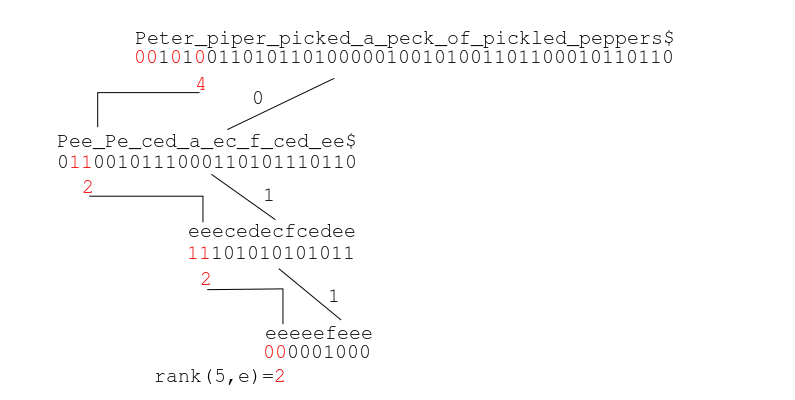
\includegraphics[width=1\textwidth]{Figures/graph2.png}
  \end{center}
\end{table}

\section{FM-Index}

FM-index(Full-text index in Minute space) is a compressed full-text substring index based on the Burrows-Wheeler Transform, with some similarities to the suffix array. It was created by (Paolo et al., 2001 \cite{paolo2001}) who describe it as an opportunistic data structure as it allows compression of the input text while still permitting fast substring queries.
It can be used to efficiently find the number of occurrences of a pattern within the compressed text, as well as locate the position of each occurrence. Both the query time and storage space requirements are sublinear with respect to the size of the input data. In contrast, the FM-index is a compressed self-index, which means that it compresses the data and indexes it at the same time.

\subsection{Suffix Arrays}

There is a variety of Suffix Array construction algorithms, including some \(O(N)\) ones (Puglisi et al., 2007 \cite{puglisi2007}). However, we will explain it from the most common (and intuitive) angle. In its simplest form, a suffix array can be constructed for a string \(S[1..N]\) like so:

\ \ \ \ 1. Construct an array of pointers to all suffixes \(S[1..N],S[2..N],…,S[N..N]\).

\ \ \ \ 2. Sort these pointers by the lexicographical (i.e. alphabetical) ordering of their associated suffixes.

For example, the sorting of the string \('abracadabra'\) with terminating character '\$' would look like this in Table \ref{ex:gsa}:

\begin{table}[!htp]
  \caption{Get Suffix Array}
  \label{ex:gsa}
  \begin{center}
    \begin{tabular}{c|c|c|c}
      \hline
      \hline
      index & string & sa & string \\
      \hline
      1 & abracadabra\$ & 12 & \$ \\
      \hline
      2 & bracadabra\$ & 11 & a\$ \\
      \hline
      3 & racadabra\$ & 8 & abra\$ \\
      \hline
      4 & acadabra\$ & 1 & abracadabra\$ \\
      \hline
      5 & cadabra\$ & 4 & acadabra\$ \\
      \hline
      6 & adabra\$ & 6 & adabra\$ \\
      \hline
      7 & dabra\$ & 9 & bra\$ \\
      \hline
      8 & abra\$ & 2 & bracadabra\$ \\
      \hline
      9 & bra\$ & 5 & cadabra\$ \\
      \hline
      10 & ra\$ & 7 & dabra\$ \\
      \hline
      11 & a\$ & 10 & ra\$ \\
      \hline
      12 & \$ & 3 & racadabra\$ \\
      \hline
    \end{tabular}
  \end{center}
\end{table}

\subsection{Burrows-Wheeler Transform}

The Burrows-Wheeler Transform (BWT) is a was developed by Burrows and Wheeler to reversibly permute a string in such a way that characters from repeated substrings would be clustered together. It was useful for compression schemes such as run-length encoding.
It is not the point of this article to explain how it works, but it is closely linked to Suffix Arrays: \(BWT[i] = S[SA[i] {-} 1]\), for the original string S, suffix array SA, and Burrows-Wheeler Transform string BWT. In other words, the ith symbol of the BWT is the symbol just before the ith suffix.
The BWT also lets us reconstruct the original string S, allowing us to discard the original document – indexes with this property are known as self indexes, which introduced by (Paolo et al., 2005 \cite{paolo2005}).

An FM-index is created by first taking the BWT of the input text. For example, the BWT of the string T = "abracadabra" is "ard\$rcaaaabb", and here it is represented by the matrix M in Table \ref{ex:mm} where each row is a rotation of the text that has been sorted. The transform corresponds to the last column labeled L.

\begin{table}[!htp]
  \caption{Matrix M}
  \label{ex:mm}
  \begin{center}
    \begin{tabular}{c|c|c}
      \hline
      \hline
      F & String & L \\
      \hline
      \$ & abracadabr & a \\
      \hline
      a & \$abracadab & r \\
      \hline
      a & bra\$abraca & d \\
      \hline
      a & bracadabra & \$ \\
      \hline
      a & cadabra\$ab & r \\
      \hline
      a & dabra\$abra & c \\
      \hline
      b & ra\$abracad & a \\
      \hline
      b & racadabra\$ & a \\
      \hline
      c & adabra\$abr & a \\
      \hline
      d & abra\$abrac & a \\
      \hline
      r & a\$abracada & b \\
      \hline
      r & acadabra\$a & b \\
      \hline
    \end{tabular}
  \end{center}
\end{table}

The BWT in itself allows for some compression with, for instance, move to front and Huffman encoding, but the transform has even more uses. The rows in the matrix are essentially the sorted suffixes of the text and the first column F of the matrix shares similarities with suffix arrays. How the suffix array relates to the BWT lies at the heart of the FM-index.

It is possible to make a last-to-first column mapping \(LF(i)\) from a character \(L[i]\) to \(F[j]\), with the help of a table \(C[c]\) and a function \(Occ(c, k)\). \(C[c]\) is a table that, for each character c in the alphabet, contains the number of occurrences of lexically smaller characters in the text. The function \(Occ(c, k)\) is the number of occurrences of character c in the prefix \(L[1..k]\). (Paolo et al., 2005 \cite{paolo2005}) showed that it is possible to compute \(Occ(c, k)\) in constant time.

The last-to-first mapping can now be defined as \(LF(i) = C[L[i]] + Occ(L[i], i)\). For instance, on row 9, \(L\) is a and the same a can be found on row 5 in the first column \(F\), so \(LF(9)\) should be 5 and \(LF(9) = C[a] + Occ(a, 9) = 5\). For any row i of the matrix, the character in the last column \(L[i]\) precedes the character in the first column \(F[i]\) also in T. Finally, if \(L[i] = T[k]\), then \(L[LF(i)] = T[k - 1]\), and using the equality it is possible to extract a string of \(T\) from \(L\).

The FM-index itself is a compression of the string \(L\) together with \(C\) and \(Occ\) in some form, as well as information that maps a selection of indices in \(L\) to positions in the original string \(T\).

\section{Fuzzy-Search Algorithms}

Let's briefly introduce our search algorithms. When we get a search query, we divide it to several terms. Each term is given a score, correspond to it's significance. Then search each term in FM-Index to get it's range. Do union operation with all term's range, and get K most related result as our final result.

\subsection{Build FM-Index}

We have \(N\) documents in our database whose text is \(t1,t2...tN\), \(T\) is contection of these text with terminating character \(\$\) for each text, as \(T=t1\$t2\$...tN\$\). Do BWT with \(T\) could get a FM-Index stored in Wavelet Tree, our searching based on this data structure.

\subsection{Get terms from search query}

Search query should be tokenize into terms, and we use the vector of terms to do next operation. Score terms would help us to rank the search result, higher score means more significance. For example, query is 'white shirt', 'shirt' have higher score than 'white', result contains only 'shirt' would rank higher than that contains only 'white' because we prefer 'yellow shirt' than 'white car'. It's just a small part of rank, we won't discuss more about rank in this article. Terms in a dictionary of brand\&good have the highest score, terms in a usual dictionary have lower score, terms construction as bigram or others have the lowest score.

\subsection{Backward search for each term}

Since any pattern \(P\) in \(S\) (the original string) is a prefix of a suffix (our Suffix Array stores suffixes), and the suffixes are lexicographically ordered, all occurrences of a search pattern \(P\) lie in a contiguous portion of the Suffix Array.
Backward search instead utilises the BWT in a series of paired rank queries (which can be answered with a Wavelet Tree), improving the query performance considerably. Backward search issues p pairs of rank queries, where p denotes the length of the pattern P. The paired rank queries are:

\begin{equation}
  \label{ex:equation_bs}
  \begin{aligned}
    &s' = C[P[i]] + rank(s {-} 1, P[i]) + 1 \\
    &e' = C[P[i]] + rank(e, P[i])
  \end{aligned}
\end{equation}

\(C\) is a lookup table containing the count of all symbols in our alphabet which sort lexicographically before \(P[i]\).
Where \(s\) denotes the start of the range and \(e\) is the end of the range. Initially \(s=1\) and \(e=N\). Index variable \(i\) starts at \(p\), decreases to 1, then get the answer. If \(e<s\) at any stage, then \(P\) doesn’t exist in \(S\). This maintains the invariant that \(SA[s..e]\) contains all the suffixes of which \(P[i..|P|]\) is a prefix, and hence all locations of \(P[i..|P|]\) in \(S\).
After backward searching, we get \([left\_range, right\_range, score]\) for each term(score get in last step), we could get the most related documents from the range set then.

\subsection{Top K Union}

Union opeartion with the range set after backward searching could get documents set which contains all terms. But in most cases, there is no document hits all terms in query, thus we want to get the document which have higher score that means higher relevance with the query. We name this operation 'top k union', as will get top k most related result after union.

Naive top k union is easy, pseudo code looks like this, then sort \(doc[]\) we could get the most related documents.

\begin{scriptsize} \begin{verbatim}
for j = 1 to range_set_size
    for i = range[j]'s left_range to range[j]'s right_range
        doc[i]'s score += score[j];
\end{verbatim} \end{scriptsize}

The time complexity is \[O(range\_set\_size\ *\ (range\_right\ -\ range\_left)) + O(sort\ all\ documents)\] and space complexity is \(O(document\ number)\), assume we have N = 100 million document, \(range\_right - range\_left\) could be at most \(N\), and a query contains at most 20 terms, the time complexity is \(O(10^8 * 20)\) and space complexity is \(O(10^8)\), both is too large.

Do you remember the Wavelet Tree? It perform perfect in backward search, and combined with heuristic searching, it could give us a excellent solution in top k union also.

Retrieve data structure of the Wavelet Tree in FM-Index, tree's root stores all text's BWT, partition it level by level, and leaf denotes document.
We define 'status' by a range set, a tree node, and a score, that means in the current node, ranges in the range set is available, and the score is the sum of all available ranges. For example, the initial status's range set is the range set after backward search which corresponding each term, node is tree's root, that means all range is available for the root, score is the sum of all terms in query.
For each status, we could derive status from it. Range will be partition into 2 ranges in the next level, one for 0 and another for 1, corresponding node is current node's left child and right child. Sometimes a derived status have a \(NULL\) range set, we should drop this status because no documents hit any terms in this node's subtree.
Every time we choose a status with highest score to derive, when status' node is a leaf, we get one result document. It's easy to find that the nth document we get has the nth highest score. It will be stopped when we get k document or all status has been derived. That is the mainly meaning of 'fuzzy search', when couldn't find document hits all terms, we could get the top k most related. Of course the document hits all terms have the highest score and won't be losen.

Pruning in searching is needed as the intermediate result is too large, we use a interval heap which key is score to store status, that could help us to get the status with highest/lowest score in \(O(1)\), and heap size is delimited to specified \(MAX\_SIZE\), when heap size reaches \(MAX\_SIZE\), we can replace the status with lowest score to a new status in \(O(log(MAX\_SIZE))\).
Pseudo code of top k union looks like follow.

\begin{scriptsize} \begin{verbatim}
heap_insert(original_range_set, root);
while(result_size < k)
{
    top_status = heap_get_max();
    if (top_status->root == leaf)
    {
        result_add(top_status);
    }
    else
    {
        for i = 0 to top_status->range_size
        {
            left/right_range = get left/right child range from top_status;
            if (left/right_range != NULL)
            {
                add left/right_range to left/right_status;
                add range's score to left/right_status;
            }
        }

        if (left/right_status != NULL and heap->size < MAX_SIZE)
            heap_insert(left/right_range);
        else if (left/right_range->score > heap_get_min()->score)
            heap_replace_min(left/right_range);
    }
}
\end{verbatim} \end{scriptsize}

\(Get\ left/right\ child\ range\) operation cost constant time as rank in a Wavelet Tree's node cost constant. We have to do it \(range\_set\_size\) times for each status, and status number is up to node number in the Wavelet Tree, equals to \(2*N\). The time complexity is \(O(range\_set\_size * N)\).
We have to store \(range\_set\_size\) ranges for each status, and status in interval heap is up to \(MAX\_SIZE\), space complexity is \(O(range\_set\_size * MAX\_SIZE)\).
It seems that time complexity is large than the naive version, but in parctise, as used pruning, status we traversed is much less than \(N\), usually less than \(N/20\). In practise we set \(MAX\_SIZE\) to \([1000..10000]\), the space complexity is much smaller than the naive version too.

\subsection{Major and Minor Terms}

Major and minor feature is used for getting better result in searching. After setting score for each term, we move significant terms(often with high score) into major set and the rest into minor set. Each returned doc contains all the major terms and any number of minor terms, thus this is a half-intersection half-union algorithm. The intersection part makes bare branches pruned much faster so that entire search performance accelerated by 3 times.

Pseudo code of the improved top k union looks like follow.

\begin{scriptsize} \begin{verbatim}
heap_insert(original_range_set, root);
while(result_size < k)
{
    top_status = heap_get_max();
    if (top_status->root == leaf)
    {
        result_add(top_status);
    }
    else
    {
        for i = 0 to top_status->major_size
        {
            left/right_range = get left/right child range from top_status;
            if (left/right_status != NULL && left/right_range != NULL)
            {
                add left/right_range to left/right_status;
                add range's score to left/right_status;
            }
            else
            {
                left/right_status = NULL;
            }
        }

        for i = top_status->major_size to top_status->range_size
        {
            left/right_range = get left/right child range from top_status;
            if (left/right_status != NULL && left/right_range != NULL)
            {
                add left/right_range to left/right_status;
                add range's score to left/right_status;
            }
        }

        if (left/right_status != NULL and heap->size < MAX_SIZE)
            heap_insert(left/right_range);
        else if (left/right_range->score > heap_get_min()->score)
            heap_replace_min(left/right_range);
    }
}
\end{verbatim} \end{scriptsize}

\subsection{Synonym}

Synonym searching means that we could get result documents which hits the synonym of term. For example, text contains only 'LV bag', query is 'Louis Vuitton bag', we could get it under synonym searching, obviously it missing in normal searching.

We build a dictionary of synonym from the SCD first, that will help us to expand original term to a synonym term set for each term, set synonym's score little lower than the original one. Then do backward search with new term set.
In top k union, we calculate status' score for each synonym term set once, that means if more than one term in the same synonym set hit a status, only the highest score will be added.

\chapter{In-memory Inverted Index}
\lhead{Chapter 5. \emph{In-memory Inverted Index}} % this is for the header on each page - perhaps a shortened title
For text retrieval systems, the assumption that all data structures reside in main memory is increasingly common. To achieve optimal performance, we adopted a state-of-art in-memory inverted index --- Zambezi~\cite{Asadi_Lin_IRJ2012,Asadi_Lin_TOIS2013,Asadi_etal_TKDE2013,Asadi_Lin_SIGIR2013}. Zambezi was originally designed for twitter's real-time search. It supports incremental index and several retrieval algorithms. In addition, we applied some enhancements to make it more versatile.

\section{Zambezi}

\subsection{Basic Incremental Indexing Algorithm}
\label{section:algo:basic}

\begin{figure*}[t]
  \begin{center}
    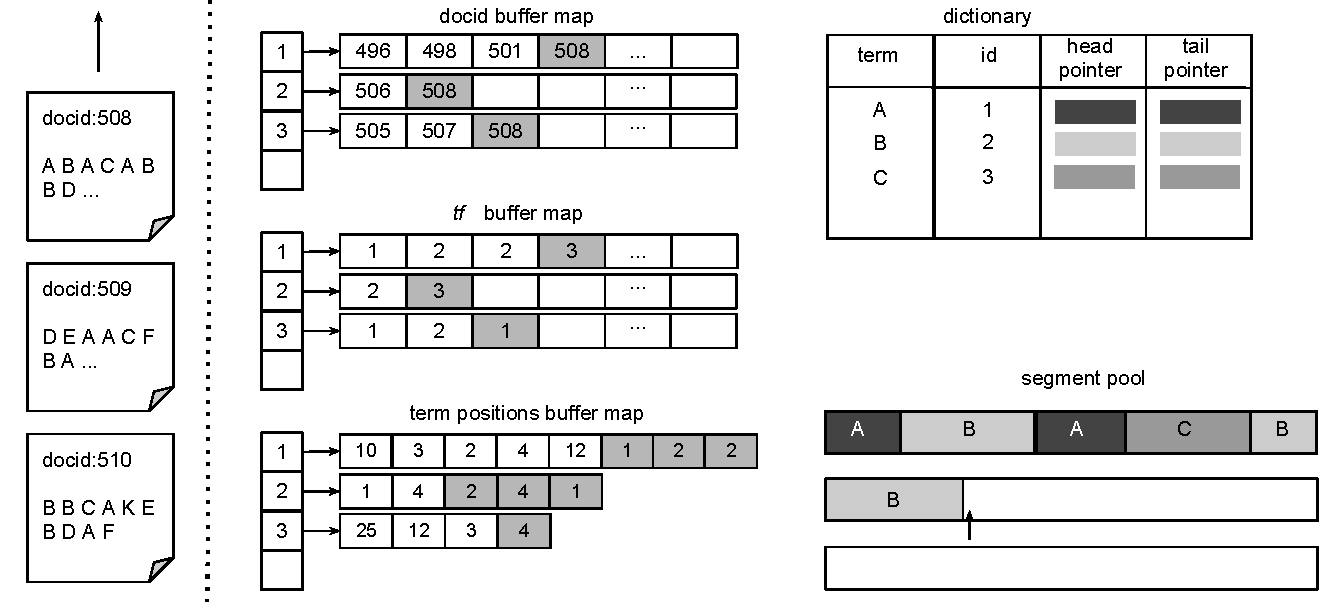
\includegraphics[width=0.8\textwidth]{Figures/IndexStructure.pdf}
  \end{center}
  \caption{A snapshot of our indexing algorithm. In the middle we have buffer maps for storing docids, \textit{tf}s, and term positions: the gray areas show elements inserted for document 508, the current one to be indexed. Once the buffer for a term fills up, an inverted list segmented is assembled and added to the end of the segment pool and linked to the previous segment via addressing pointers. The dictionary maps from terms to term ids and holds pointers to the head and tail of the inverted list segments in the segment pool.
  \label{figure:indexStructure}}
\end{figure*}

Our indexer consists of three main components, depicted in Figure~\ref{figure:indexStructure}: the dictionary, buffer maps, and the segment pool. The basic indexing approach is to accumulate postings in the buffer maps in an uncompressed form until the buffer fills up, and then to ``flush'' the contents to the segment pool, where the final compressed postings lists reside. Note that in this approach the inverted lists are discontiguous; we return to address this issue in Section~\ref{section:algo:contiguity}.

The dictionary is implemented as a hash table with a bit-wise hash function~\cite{RamakrishnaDASFAA1997} and the move-to-front technique~\cite{WilliamsSPE2001}, mapping terms (strings) to integers term ids (see~\cite{ZobelIPL2001} for a study that compares this to other approaches). There is nothing noteworthy about our dictionary implementation, and we claim no novelty in this design. The dictionary additionally holds the document frequency (\textit{df}) for each term, as well as a head and tail pointer into the segment pool (more details below). In our implementation, term ids are assigned sequentially as we encounter new terms.

A \textit{buffer map} is a one-to-one mapping from term ids to arrays of integers (the buffers). Since term ids increase monotonically, a buffer map can be implemented as an array of pointers, where each index position corresponds to a term id, and the pointer points to the associated buffer. The array of pointers is dynamically expanded to accommodate more terms as needed. To construct a positional index, we build three buffer maps: the document id (docid) map, the term frequency (\textit{tf}) map, and the term positions map. As the names suggest, the docid map accumulates the document ids of arriving documents, the \textit{tf} map holds term frequencies, and the term positions map holds term positions. There is a one-to-one correspondence between entries in the docid map and entries in the \textit{tf} map (for each term that occurs in a document, there is exactly one term frequency), but a one-to-many correspondence between entries in the docid map and entries in the term positions map (there are as many 
term positions in each document as the term frequency).

In the indexing loop, the algorithm receives an input document, parses it to gather all term frequencies and term positions (relative to the current document, starting from one) for all unique terms, and then iterates over these unique terms, inserting the relevant information into each buffer map. Whenever we encounter a new term, the algorithm initializes an empty buffer in each buffer map for the corresponding term id. Initially, the buffer size is set to the block size $b$ that will eventually be used to compressed the data (leaving aside an optimization we introduce below to control the vocabulary size). Following best practice today, we use PForDelta~\cite{ZukowskiICDE2006,Yan_etal_WWW2009}, with the recommended block size of $b=128$. The term positions map expands one block at a time when it fills up to accommodate more positions. When the docid buffer for a term fills up, we ``flush'' all buffers associated with the term, compressing the docids, term frequencies, and term positions into what we call 
an inverted list segment, described below:

Each inverted list segment begins with a run of docids, gap-compressed using PForDelta; call this $D$. By design, the docids occupy exactly one PForDelta block. Next, we compress the term frequencies using PFor; call this $F$. Note that term frequencies cannot be gap-compressed, so they are left unmodified. Finally, we process the term positions, which are also gap-encoded, relative to the first term position in each document. For example, if in $d_1$ the term was found at positions $[1, 5, 9]$ and in $d_2$ the term was found at positions $[3, 16]$, we would code $[1, 4, 4, 3, 13]$. The term positions can be unambiguously reconstructed from the term frequencies, which provide offsets into the array of term positions. Since the term positions array is likely longer than $b$, the compression block size, the term positions occupy multiple blocks. Call the blocks of term positions $P_1 \ldots P_m$.

Finally, all the data are packed together in a contiguous block of memory as follows:

\begin{displaymath}
  \begin{array}{l}
    \left[\; |D|,\; D,\; |F|,\; F,\; \{ |P_i|,\; P_i \}_{0 \leq i < m} \right] \\
  \end{array}
\end{displaymath}

\noindent where the $|\cdot|$ operator returns the length of its argument. Since all the data are tightly packed in an otherwise undelimited array, we need to explicitly store the lengths of each block to properly decode the data during retrieval.

Each inverted list segment is written at the end of the segment pool, which is where the compressed inverted index ultimately resides. Conceptually, the segment pool is an bounded array with a pointer that keeps track of the current ``end'', but in practice the pool is allocated in large blocks and dynamically expanded as necessary. In order to traverse a term's postings during query evaluation, we need to ``link'' together the discontiguous segments. The first time we write a segment for a term id, we add its address (byte offset in the segment pool) to the dictionary, which serves as the ``head'' pointer (the entry point to postings traversal). In addition, we prepend to each segment the address (byte offset position in the segment pool) of the next segment in the chain. This means that every time we insert a new segment for a term, we have to go back and correct the ``next pointer'' for the last segment. We leave the next pointer blank for a newly-inserted segment to mark the end of the postings list for 
a term; this location is stored in the ``tail pointer'' in the dictionary. Once the indexer has processed all documents, the remaining contents of the buffer maps are flushed to the segment pool in the same manner. By default, we build full positional indexes, but our implementation has an option to disable the term position buffers if desired. In this case, the inverted list segments will be smaller, but other aspects of the algorithm remain exactly the same.

Conceptually speaking, the postings list for each term is a linked list of inverted list segments, where each of the segments is laid out in discontiguous monotonically-increasing byte offset positions in the segment pool and linked together with addressing pointers. Segments corresponding to different terms are arbitrarily interleaved in the segment pool. What are the implications of this design? On the positive side, all data in the segment pool are ``tightly packed'' for maximum efficiency in memory utilization: there are no empty regions and there is no need for special delimiters. During indexing we guarantee that there is no heap fragmentation, which may be a possibility if we simply used \texttt{malloc} to allocate space for each inverted list segment. On the negative side, postings traversal becomes an exercise in pointer chasing across the heap, without any predictable access patterns that will aid in processor pre-fetching across segment boundaries. Thus, as a query evaluation algorithm consumes 
postings, it is likely to encounter a cache miss whenever it reaches the end of a segment, since it has to follow a pointer. On the other hand, it is not entirely clear if this cache miss is a major concern: since PForDelta is block-based, postings are decompressed in blocks even if the inverted lists are contiguously stored in memory.

In addition to ``flushing to memory'' (i.e., the segment pool) as opposed to flushing to disk, the operation of our indexer is fundamentally different from previous designs. In previous approaches, the in-memory buffer is completely flushed when the capacity limit is reached, which means that inverted lists associated with \textit{all} terms are written to disk. In contrast, we only flush data associated with the term id whose buffer has reach capacity.

One final optimization detail: we control the size of the term space by discarding terms that occur fewer than ten times (an adjustable document frequency threshold). This is accomplished as follows: instead of creating a buffer of length $b$ when we first encounter a new term, we first allocate a small buffer equal to the \textit{df} threshold. We buffer postings for new terms until the threshold is reached, after which we know that the term will make it into the final dictionary, and so we reallocate a buffer of length $b$. This two-step process reduces memory usage substantially since there are many rare terms in web collections.

\subsection{Segment Contiguity}
\label{section:algo:contiguity}

It is clear that our baseline indexing algorithm generates discontiguous inverted list segments. In order to create contiguous inverted lists, we would need an algorithm to rearrange the segments once they are written to the segment pool. Following the ``remerging'' idea in disk-based incremental indexing, we might merge multiple discontiguous segments belonging to the same term id and transfer them to another region in memory, repeating if necessary. Alternatively, when writing an inverted segment to the segment pool, we might leave some empty space---but since no pre-allocation policy can be prescient, we will either leave too much empty space (wasting memory) or not leave enough (necessitating further copying). These basic designs have been explored in the context of on-disk incremental indexing, but we argue that the issues become more complex in memory because we do not have an intermediate abstraction of the file---the indexing algorithm must explicitly manage memory addresses. This amounts to 
implementing \texttt{malloc} and \texttt{free} for inverted list segments, which is a non-trivial task.

Before going down this path, however, we first examined the extent to which contiguous segments would improve retrieval efficiency, from better reference locality, pre-fetch cues provided to the processor, etc. Let us assume we have an oracle that tells us exactly how long each inverted list is going to be, so that we can lay out the segments end-to-end, without any wasted memory. We simulate this oracle condition by building the inverted index as normal, and then performing in-memory post-processing to lay out all the inverted list contiguously. Obviously, in a real incremental indexing scenario, this is not a workable option, but this simple experiment allows us to measure the ideal performance from the perspective of query evaluation. Thus, we can establish two retrieval efficiency bounds---the query evaluation time on arbitrarily discontiguous inverted lists (the baseline algorithm) and on contiguous inverted lists (the upper bound on query evaluation speed).

Using these two efficiency bounds as guides, we developed a simple yet effective approach to achieving increasingly better approximations of contiguous postings lists. Instead of moving compressed segments around after they have been added to the segment pool, we change the memory allocation policy for the buffer maps. In the limit, if we increased buffer map sizes so that they are large enough to hold the entire document collection in uncompressed form, it is easy to see how we could build contiguous inverted list segments. As it turns out, we do not need to go to such extremes.

In our strategy, whenever the docid buffer for a term becomes full (and thus compressed and flushed to the segment pool), we expand that term's docid and \textit{tf} buffers by a factor of two (still allowing the term positions buffer to grow as long as necessary). This means that after the first segment of a term is flushed, new docid and \textit{tf} buffers of length $2b$ replace the old ones; after the second flush, the buffer size increases to $4b$, and then $8b$, and so on. When a buffer of size $2^m b$ becomes full, the buffer is broken down to $2^m$ segments, each segment is compressed as described earlier, and all $2^m$ segments are written at the end of the segment pool contiguously. This strategy allows long postings to become increasingly contiguous, without wasting space to pre-allocate large buffers to hold terms that turn out to be rare.

To prevent buffers from growing indefinitely and to control the memory pressure, we set a cap on the length of docid and \textit{tf} buffers. That is, if the cap is set to $2^m b$, then when the buffer size for a term reaches that limit, it is no longer expanded. This means that the maximum number of contiguous segments allowed in the segment pool is $2^m$. We experimentally show that for relatively small values of $m$, around 6 or 7, we achieve query evaluation speeds that are statistically indistinguishable from having an index with fully-contiguous inverted lists (i.e., the oracle condition). The tradeoff of this approach is that we require more transient working memory during the indexing process, and that impacts the size of the collection that we can index. However, we experimentally show that the additional memory requirements for implementing this approach are reasonable. Note that for on-disk incremental indexing algorithms, the strategy of increasing the in-memory buffer size is generally not 
considered since those algorithms operate under an assumption of limited memory. In our case, we are simply changing the allocation between transient working memory for performing document inversion and the final index structures.

\begin{table*}[t]
  \setlength{\tabcolsep}{1.5pt}
  \renewcommand{\arraystretch}{1.5}
  \centering
  \scriptsize
  \begin{tabular}{|c|l||c|c|c|c|c|c|c|c||c|}
    \hline
    & Query & $1b$ & $2b$ & $4b$ & $8b$ & $16b$ & $32b$ & $64b$ & $128b$ & Contiguous\\
    \hline
    \hline
    \multirow{2}{0.15cm}{\rotatebox{90}{\tiny Gov2}}
    & Terabyte & 14.4 ($\pm$0.2) & 14.2 ($\pm$0.1) & 13.9 ($\pm$0.1) & 13.6 ($\pm$0.1)
    & 13.3 ($\pm$0.1) & 13.2 ($\pm$0.1) & 13.1 ($\pm$0.1) & 13.1 ($\pm$0.1) & 13.1 ($\pm$0.1) \\
    & AOL & 20.2 ($\pm$0.4) & 19.7 ($\pm$0.1) & 19.3 ($\pm$0.2) & 19.0 ($\pm$0.3) & 18.8 ($\pm$0.3)
    & 18.7 ($\pm$0.5) & 18.4 ($\pm$0.2) & 18.3 ($\pm$0.1) & 18.2 ($\pm$0.2) \\
    \hline
    \hline
    \multirow{2}{0.15cm}{\rotatebox{90}{\tiny Clue}}
    & Terabyte & 49.7 ($\pm$0.2) & 47.1 ($\pm$0.1) & 45.9 ($\pm$0.4) & 44.4 ($\pm$0.5) &
    42.9 ($\pm$0.4) & 42.0 ($\pm$0.3) & 41.6 ($\pm$0.1) & 41.6 ($\pm$0.4) & 41.3 ($\pm$0.1) \\
                    & AOL & 87.5 ($\pm$1.6) & 83.2 ($\pm$0.5) & 80.7 ($\pm$0.3) & 75.5 ($\pm$0.5)
    & 75.7 ($\pm$0.8) & 75.8 ($\pm$0.3) & 75.2 ($\pm$0.2) & 75.0 ($\pm$0.6) & 75.3 ($\pm$1.2) \\
    \hline
  \end{tabular}
  \caption{Average query latency (in milliseconds) for postings intersection using SvS with different buffer length settings. Results are averaged across 5 trials, reported with 95\% confidence intervals.
  \label{table:queryLatency}}
\end{table*}

\subsection{Query Latency}

Table~\ref{table:queryLatency} summarizes query latency for conjunctive query processing (postings intersection with SvS). The average latency per query is reported in milliseconds across five trials along with 95\% confidence intervals. Each column shows different indexing conditions: $1b$ is the baseline algorithm presented in Section~\ref{section:algo:basic} (linked list of inverted list segments). Each of $\{2, 4, 8 \ldots 128\}b$ represents a different upper bound in the buffer map growing strategy described in Section~\ref{section:algo:contiguity}. The final column marked ``contiguous'' denotes the oracle condition in which all postings are contiguous; this represents the ideal performance.

From these results, we see that, as expected, discontiguous postings lists ($1b$) yield slower query evaluation: on Gov2, queries are approximately 10\% slower, while for ClueWeb09, the performance dropoff ranges from 16\% to 20\%.  For higher values of $b$, we allow the buffer maps to increase in length: at $32b$, query evaluation performance is statistically indistinguishable from the performance upper bound (i.e., confidence intervals overlap). That is, we only need to arrange inverted list segments in relatively small groups of 32 to achieve ideal performance. Later, we quantify the memory requirements of allocating larger buffer maps.

\begin{figure*}[t]
  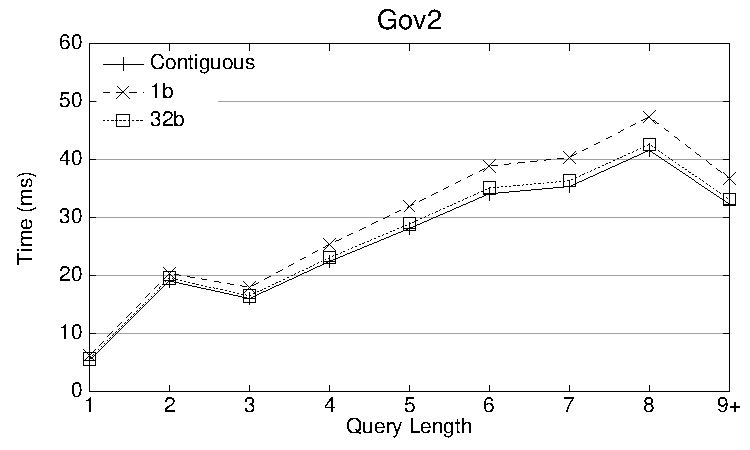
\includegraphics[width=0.49\linewidth]{Figures/latency_gov2_aol.pdf}
  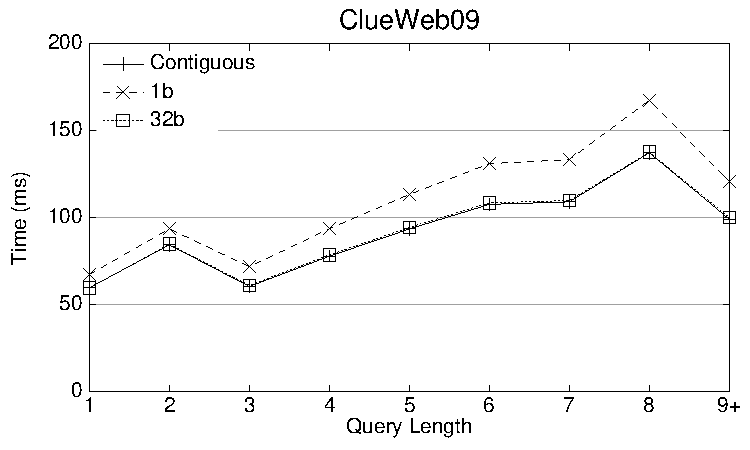
\includegraphics[width=0.49\linewidth]{Figures/latency_clue_aol.pdf}
  \caption{Query latency using SvS for the AOL query set, by query length for different buffer length settings.
  \label{figure:queryLatency}}
\end{figure*}

Figure~\ref{figure:queryLatency} illustrates query latency by query length, for the AOL query set on Gov2 and ClueWeb09, using different conditions. Not surprisingly, the latency gap between contiguous and the $1b$ condition widens for longer queries. On the other hand, the difference between a contiguous index and the $32b$ condition is indistinguishable across all query lengths---the lines practically overlap in the figures.

\begin{table}[t]
  \setlength{\tabcolsep}{3.5pt}
  \centering
  \small
  \begin{tabular}{|c|l||c|c|c|}
    \hline
    & Query & $1b$ & $32b$ & Contiguous\\
    \hline
    \hline
    \multirow{2}{0.1cm}{\rotatebox{90}{\tiny Gov2}}
    & Terabyte & 65.0 ($\pm$0.4) & 62.5 ($\pm$0.8) & 62.0 ($\pm$0.4) \\
    & AOL & 103.5 ($\pm$0.5) & 100.3 ($\pm$0.1) & 100.2 ($\pm$0.4) \\
    \hline
    \hline
    \multirow{2}{0.1cm}{\rotatebox{90}{\tiny Clue}}
    & Terabyte & 150.0 ($\pm$0.5) & 141.1 ($\pm$0.6) & 141.1 ($\pm$0.2) \\
    & AOL & 455.7 ($\pm$5.1) & 434.3 ($\pm$5.8) & 432.6 ($\pm$4.9) \\
    \hline
  \end{tabular}
  \caption{Average query latency (in milliseconds) to retrieve the top 1000 hits in terms of BM25 using WAND (5 trials, with 95\% confidence intervals).
  \label{table:queryLatency:wand}}
\end{table}

For disjunctive query processing, we used the \textsc{Wand} algorithm to retrieve the top 1000 documents using BM25. Table~\ref{table:queryLatency:wand} summarizes these experiments on different collections and queries. For space considerations, we only report results for select buffer length configurations. These results are consistent with the conjunctive processing case. A maximum buffer size of $32b$ yields query latencies that are statistically indistinguishable from a contiguous index. Note that the performance difference between fully-contiguous postings lists and $1b$ discontiguous postings lists is less than 7\%. In other words, there is much less performance degradation than in the SvS case.

As with the conjunctive query processing case, we analyzed query latency by length. The results, however, were not particularly insightful: as expected, query latency increases with length, and the performance differences between the three conditions were so small that the plots essentially overlapped. For this reason, we did not include the corresponding figures here.

\subsection{Memory Usage}

All inverted indexing algorithms require transient working memory to hold intermediate data structures. For on-disk incremental indexing algorithms, previous work has assumed that this working memory is relatively small. In our case, there is no hard limit on the amount of space we can devote to working memory, but space allocated for holding intermediate data takes away from space that can be used to store the final compressed postings lists, which limits the size of the collection that we can index for a fixed server configuration.

At minimum, our buffer maps must hold the most recent $b$ docids, term frequencies, and associated term positions (leaving aside the rare terms optimization in Section~\ref{section:algo:basic}). In our case, we set $b=128$ to match best practices PForDelta block size; any smaller value would compromise decompression performance. In order to increase the contiguity of the inverted list segments, we increase the length of the buffers, as described in Section~\ref{section:algo:contiguity}. This of course increases the space requirements of the buffer maps.

\begin{figure}[t]
  \centering
  \begin{subfigure}[b]{0.45\textwidth}
    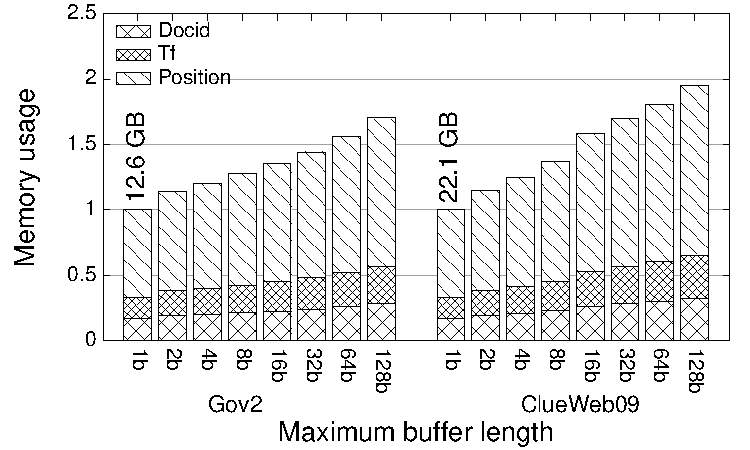
\includegraphics[width=\textwidth]{Figures/memory_usage.pdf}
    \caption{Memory required to hold all buffer maps for different buffer length settings, normalized to the $1b$ setting, on Gov2 and ClueWeb09.
    \label{figure:memoryUsage}}
  \end{subfigure}
  \begin{subfigure}[b]{0.45\textwidth}
    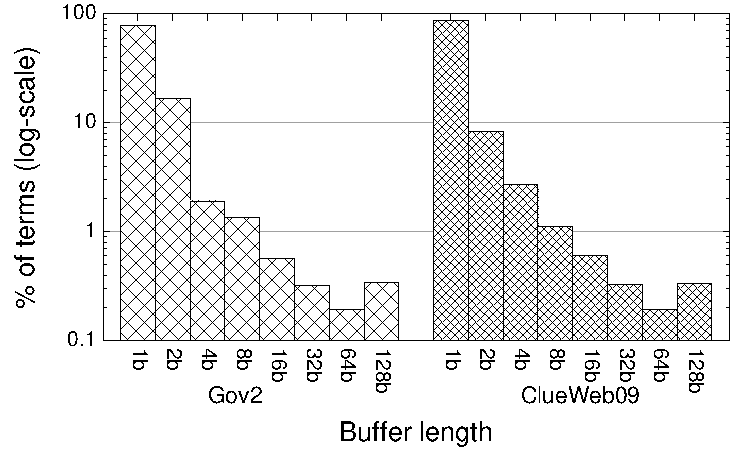
\includegraphics[width=\textwidth]{Figures/buffer_length_32b.pdf}
    \caption{Percentage of terms for which a buffer of length $m \times b$ is required, for different values of $m$, and block size $b=128$.
    \label{figure:bufferLengthDist}}
  \end{subfigure}
  \caption{Memory behavior of buffer maps.}
\end{figure}

Figure~\ref{figure:memoryUsage} shows the maximum size of the buffer maps for different contiguity configurations, broken down by space devoted to docids, term frequencies, and term positions. The reported values were computed analytically from the necessary term statistics, making the assumption that all terms reach their maximum buffer size at the same time, which makes these upper bounds on memory usage. To facilitate comparison across the two collections, we normalized the values to the $1b$ condition; in absolute terms, the total buffer map sizes are 12.6GB for Gov2 and 22.1GB for ClueWeb09. It is no surprise that as the maximum buffer length increases, the total memory requirement grows as well. At $128b$, where we allow the buffer to grow to 128 blocks of 128 32-bit integers, the algorithm requires 71\% more space for Gov2 and 95\% more space for ClueWeb09 (compared to the $1b$ condition). At $32b$, which from our previous results achieves query evaluation performance that is statistically 
indistinguishable from contiguous postings lists, we require 44\% and 70\% more memory for Gov2 and ClueWeb09, respectively.

As reference, the total size of the segment pool (i.e., size of the final index) is 31GB for Gov2 and 62GB for ClueWeb09. This means, on the Gov2 collection, setting the maximum buffer length to $1b$, $32b$ and $128b$ results in a buffer map that is approximately 41\%, 59\%, and 69\% of the overall size of the segment pool, respectively. Similarly, for ClueWeb09, the buffer map sizes are approximately 32\%, 54\%, and 63\% of the size of the segment pool, respectively. These statistics quantify the overhead of our in-memory indexing algorithms.

Note that most of the working memory is taken up by term positions; in comparison, the requirements for buffering docids and term positions are relatively modest. In all cases the present implementation uses 32-bit integers, even for term positions. We could easily cut the memory requirements for those in half by switching to 16-bit integers, although this would require us to either discard or arbitrarily truncate long documents. Ultimately, we decided not to sacrifice the ability to index long documents.

The total number of unique terms is 31M in Gov2 and 79M in ClueWeb09. Since these collections consist of web pages, most of the terms are unique and correspond to JavaScript fragments that our parser inadvertently included and other HTML idiosyncrasies; such issues are prevalent in web search and HTML cleanup is beyond the scope of this paper. Our indexer discards terms that occur fewer than 10 times, which results in a vocabulary size of 2.9M for Gov2 and 6.9M for ClueWeb09. Of these, Figure~\ref{figure:bufferLengthDist} shows the percentage of terms that require a maximum buffer length of $m \times b$, for different values of $m$ in our contiguity settings. For example, the $1b$ bar represents terms whose document frequencies are $\ge10$ but $<128$. The $2b$ bar represents terms whose document frequencies are $\ge128$ but less than $1b + 2b = 384$, and so on. The $128b$ bar represents terms whose document frequencies exceed the maximum buffer length of 128 blocks. From this we can see why significantly 
increasing the $b$ value only yields a modest increase in memory requirements.

Finally, the average size of each inverted list segment for terms with a buffer length of $1b$ is about 300 bytes; for terms that require a buffer of length of $2b$, the average length is around 600 bytes. For terms with a buffer of length $>2b$, this value is about 800 bytes. These statistics make sense since $1b$ terms may have less than a document frequency of 128, and in general, rarer terms have smaller term frequencies, and hence fewer term positions.

\section{Attribute Score Search}

To fit our requirements, we deeply customized the original Zambezi. In our implementation, each document comprises multiple attributes and we assign each attribute a respective score (details are in Chapter~\ref{chap:product_ranking}). For convenience of implementation, all attribute scores are 16-bit integers.

In the indexing loop, the indexer receives an input document consisting of a list of \(\langle attribute, score \rangle\) pairs, extracts a unique term list, and calculate the document score corresponding to each term. If a particular term exists in different attributes of a document, then the term score is the sum of scores to all the attributes in which that term exists:

\begin{equation}
  S_{\mathbf{D}, t} = \sum_{t \in \mathbf{D} | \mathcal{A}} S_{\mathcal{A}}
\end{equation}

The modified indexer has similar scheme as the original depicted in Figure~\ref{figure:indexStructure}, except that buffer maps and segment pool store docid list and score list. In application, term frequencies and term positions are not needed. Each posting segment stores a gap-compressed docid list $D$ and an uncompressed score list $S$. All the data are packed together in a contiguous block of memory as follows:

\begin{displaymath}
  \begin{array}{l}
    \left[\; |D|,\; D,\; |S|,\; S\; \right] \\
  \end{array}
\end{displaymath}

During retrieval, we intersect all term postings using SvS algorithm and calculate scores for each candidate in the common set. For a query $\mathbf{Q}$, the score for a candidate is calculated as below:

\begin{equation}
  S_{\mathbf{D}} = \sum_{t \in \mathbf{Q}} S_{\mathbf{D}, t}
\end{equation}

Then Zambezi has finished its work. The candidates and their scores are passed to reranking stage.

\section{Real-time Extension}

\subsection{Motivation}

The Zambezi indexer has limitations. Many of the techniques are tweet-specific and not applicable to the general case. For example, it assumes terms occurring less than $9$ times insignificant thus unsearchable. This assumption may be true for twitter trends but not for other data sources. In product or hotel search, the rare but useful terms may lay in buffer maps and never be flushed to segment pool. We demanded a lockless, real-time, incremental inverted index. Zambezi already proposed a good incremental scheme. Our work is to make it real-time, i.e. to make the buffer maps searchable, and retain its locklessness. This is also a future work discussed by the authors.

\subsection{Solution}

The solution is not complex. We first reimplement the buffer maps with \texttt{boost::shared\_array} and \texttt{boost::atomic} libraries. Each posting buffer is stored in a smart pointer. We use atomic operations to ensure data consistency between write(index) and read(retrieval) threads. This is a copy-on-write strategy implementation. As buffer maps is dynamically expanded as necessary, the combine use of \texttt{boost::shared\_array} and \texttt{boost::atomic} can ensure that retrieval threads are still iterating on \textbf{valid} old data while index thread allocating a new memory region.

The SvS intersection algorithm also needs to be updated to support search buffer maps. We rewrite the posting search algorithm so that it can iterate from segment pool to buffer maps (or the reverse) seamlessly.

There are other enhancements we made for this new Zambezi index:

\begin{list}{\labelitemi}{\leftmargin=1em}
\setlength{\itemsep}{-2pt}

  \item \textit{Native filter support.} We added filter handling in SvS algorithm so that filters are applied more efficient. Moreover, if filters are implemented outside retrieval algorithm, probably we can not get sufficient candidates.

  \item \textit{Better integer compressor.} We shift the PFor(Delta) compressor to the recently proposed \texttt{S4-BP128-D4} \cite{Lemire_etal_2014}. It puts compression and delta coding in a single run to reduce cache misses and exploits SIMD instructions to accelerate both. We also modified the data alignment for segment pool to 128-bit as SIMD demands.

  \item \textit{Better posting search algorithm.} The original uses \textit{galloping} search \cite{bentley1976almost} for iteration on postings list, which is nearly optimal for unbounded search over sorted list. However, with a postings segment or buffer map no longer than $4096$, the integer comparisons saved by \textit{galloping} search can not offset the cache misses which it draws in. We shift to SIMD accelerated \textit{linear} search~\cite{schani2010} instead.
\end{list}

% Chapter Template

\chapter{Search Cloud} % Main chapter title

\label{Chapter6} % for referencing this chapter elsewhere, use \ref{ChapterX}

\lhead{Chapter 6. \emph{Search Cloud}} % this is for the header on each page - perhaps a shortened title
\section{Overview}
\texttt{SF1R} could be deployed as a fully distributed search engine. Within \texttt{iZENECloud}, we have it supporting different kinds of search requests, 
some of which require non-distributed deployment while others are deployed distributedly, as shown in figure \ref{fig:searchcloud}. We call such platform
as a search cloud.
\begin{figure}[!ht]\centering
  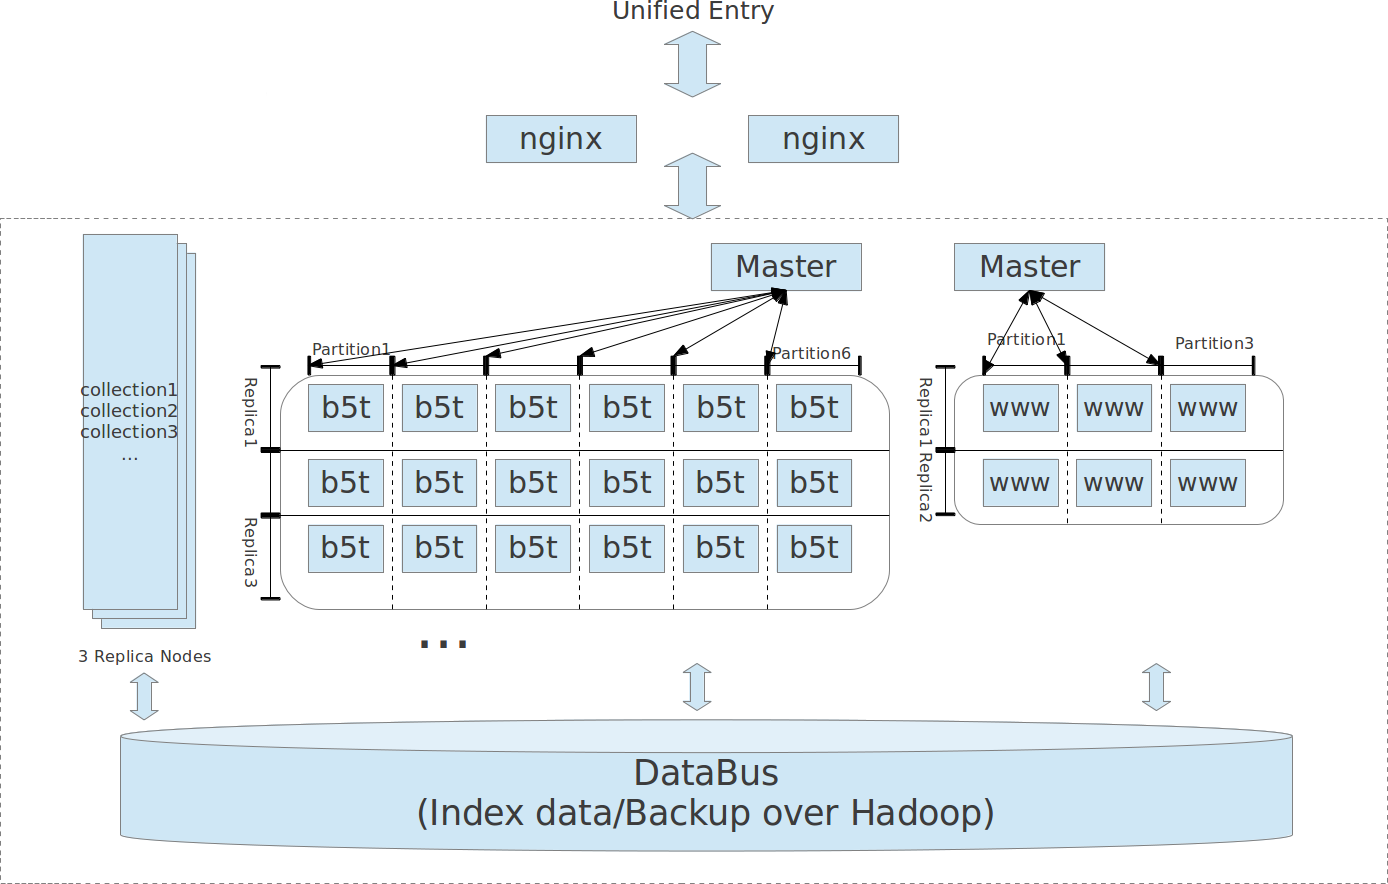
\includegraphics[width=.90\textwidth]{Figures/searchcloud.png}
  \caption{SF1R Search Cloud}\label{fig:searchcloud}
\end{figure}


The overview of \emph{Distributed SF1R} nodes is shown in \ref{fig:overview}. Each Node can have several replicas, and all the replicas in the same replica 
set have the same nodeid. We call them together as a replica set. Basically, there will be one primary node and some secondary nodes in the specific replica
set. Each node will supply the master and worker parts.

\begin{figure}[!ht]\centering
  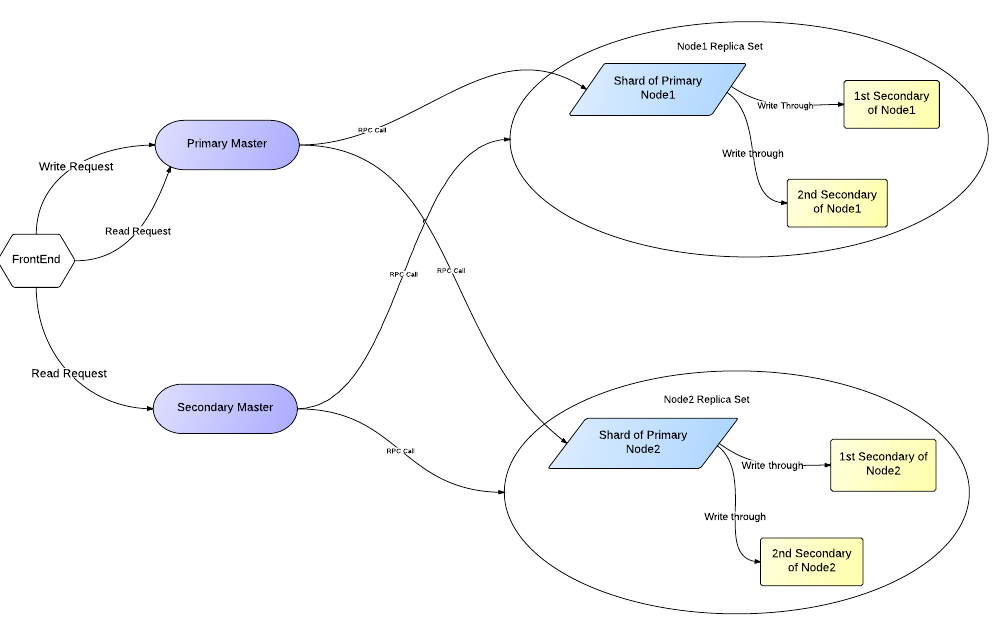
\includegraphics[width=.90\textwidth]{Figures/overview.png}
  \caption{Distributed SF1R Architecture}\label{fig:overview}
\end{figure}
\begin{figure}[!ht]\centering
  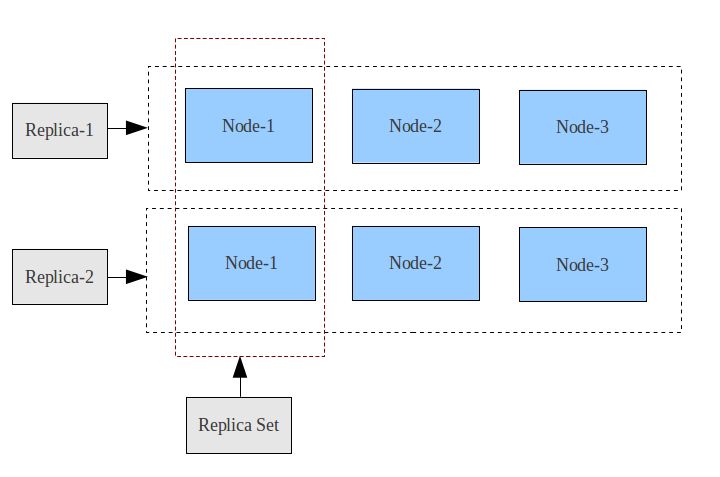
\includegraphics[width=.70\textwidth]{Figures/replica-set.png}
  \caption{Distributed SF1R Replica Set}\label{fig:replica-set}
\end{figure}

\begin{enumerate}
 \item \emph{Primary Master} \newline
   The master part on the primary node, it will take charge of distributing the search request to all shard workers and merging the results from all shard workers. And also take the charge of pulling the write request from zookeeper and distribute the write request to all shard workers on primary.

 \item \emph{Secondary Master} \newline
   The master part on the secondary node, it will take charge of distributing the search request to all shard workers and merging the results from all shard workers. And also take the charge of pushing the write request to zookeeper.
 \item \emph{Shard Worker} \newline
    The worker part on the node will do the actually work as one of shard worker and return the result to the master. For write request, the shard worker on primary node will take charge of broadcasting the request to all secondary nodes in the same replica set.
\end{enumerate}

\section{Architecture and Internal}
\subsection{The role of ZooKeeper}
    The ZooKeeper in the distributed sf1r will serve as the node activity detecting and primary electing. The distributed write queue is also used in the zookeeper to make sure all write request can be saved temporally. In sync mode, the zookeeper is used to keep the processing state of write request and notify the primary and the secondary nodes about the state changes. By using zookeeper we can make sure all nodes  will see the same topology view in the distributed sf1r since the zookeeper has implemented the PAXOS protocols to make sure the data consistency. The topology in zookeeper is as below:
\begin{lstlisting}
/                                  # Root of zookeeper namespace
|--- SF1R-[CLUSTERID]              # Root of distributed SF1 namesapce, 
                                   [CLUSTERID] is specified by user configuration.

      |--- Topology                # Topology of distributed service cluster
           |--- Replica1           # A replica of service cluster
                |--- Node1         # A SF1 node in the replica of cluster, it can be a 
                                     Master or Worker or both.
                |--- Node2
           |--- Replica2
                |--- Node1
                |--- Node2

      |--- Servers                 # Servers in topology is a master node.
           |--- Server00000000
                     |--- Search, Recommend       # A master node supply Search and 
                                                  #  Recommend service as master
           |--- Server00000001
      |--- WriteRquestQueue                       # Root of waiting write request queue
           |--- Node1                             # Waiting Write request queue for node1
                |--- WriteRequestSeq0000000000    # the waiting write request
           |--- Node2
      |--- PrimaryNodes
           |--- Node1                             # backup primary nodes for node1 
                |--- Primary0000000000            # first backup primary server as current                                                                
                                                  #  primary for replica set node1.
                |--- Primary0000000001            
           |--- Node2
                |--- Primary0000000000
                |--- Primary0000000001
      |--- WriteRequestPrepare                    # prepare root node for sync write
           |--- Node1                             # prepare for node1 in sync write.
           |--- Node2
      |--- Synchro                 # For synchronization task

\end{lstlisting} 
    
    
\subsection{The new write routine on distributed sf1r}

\begin{figure}[!ht]\centering
  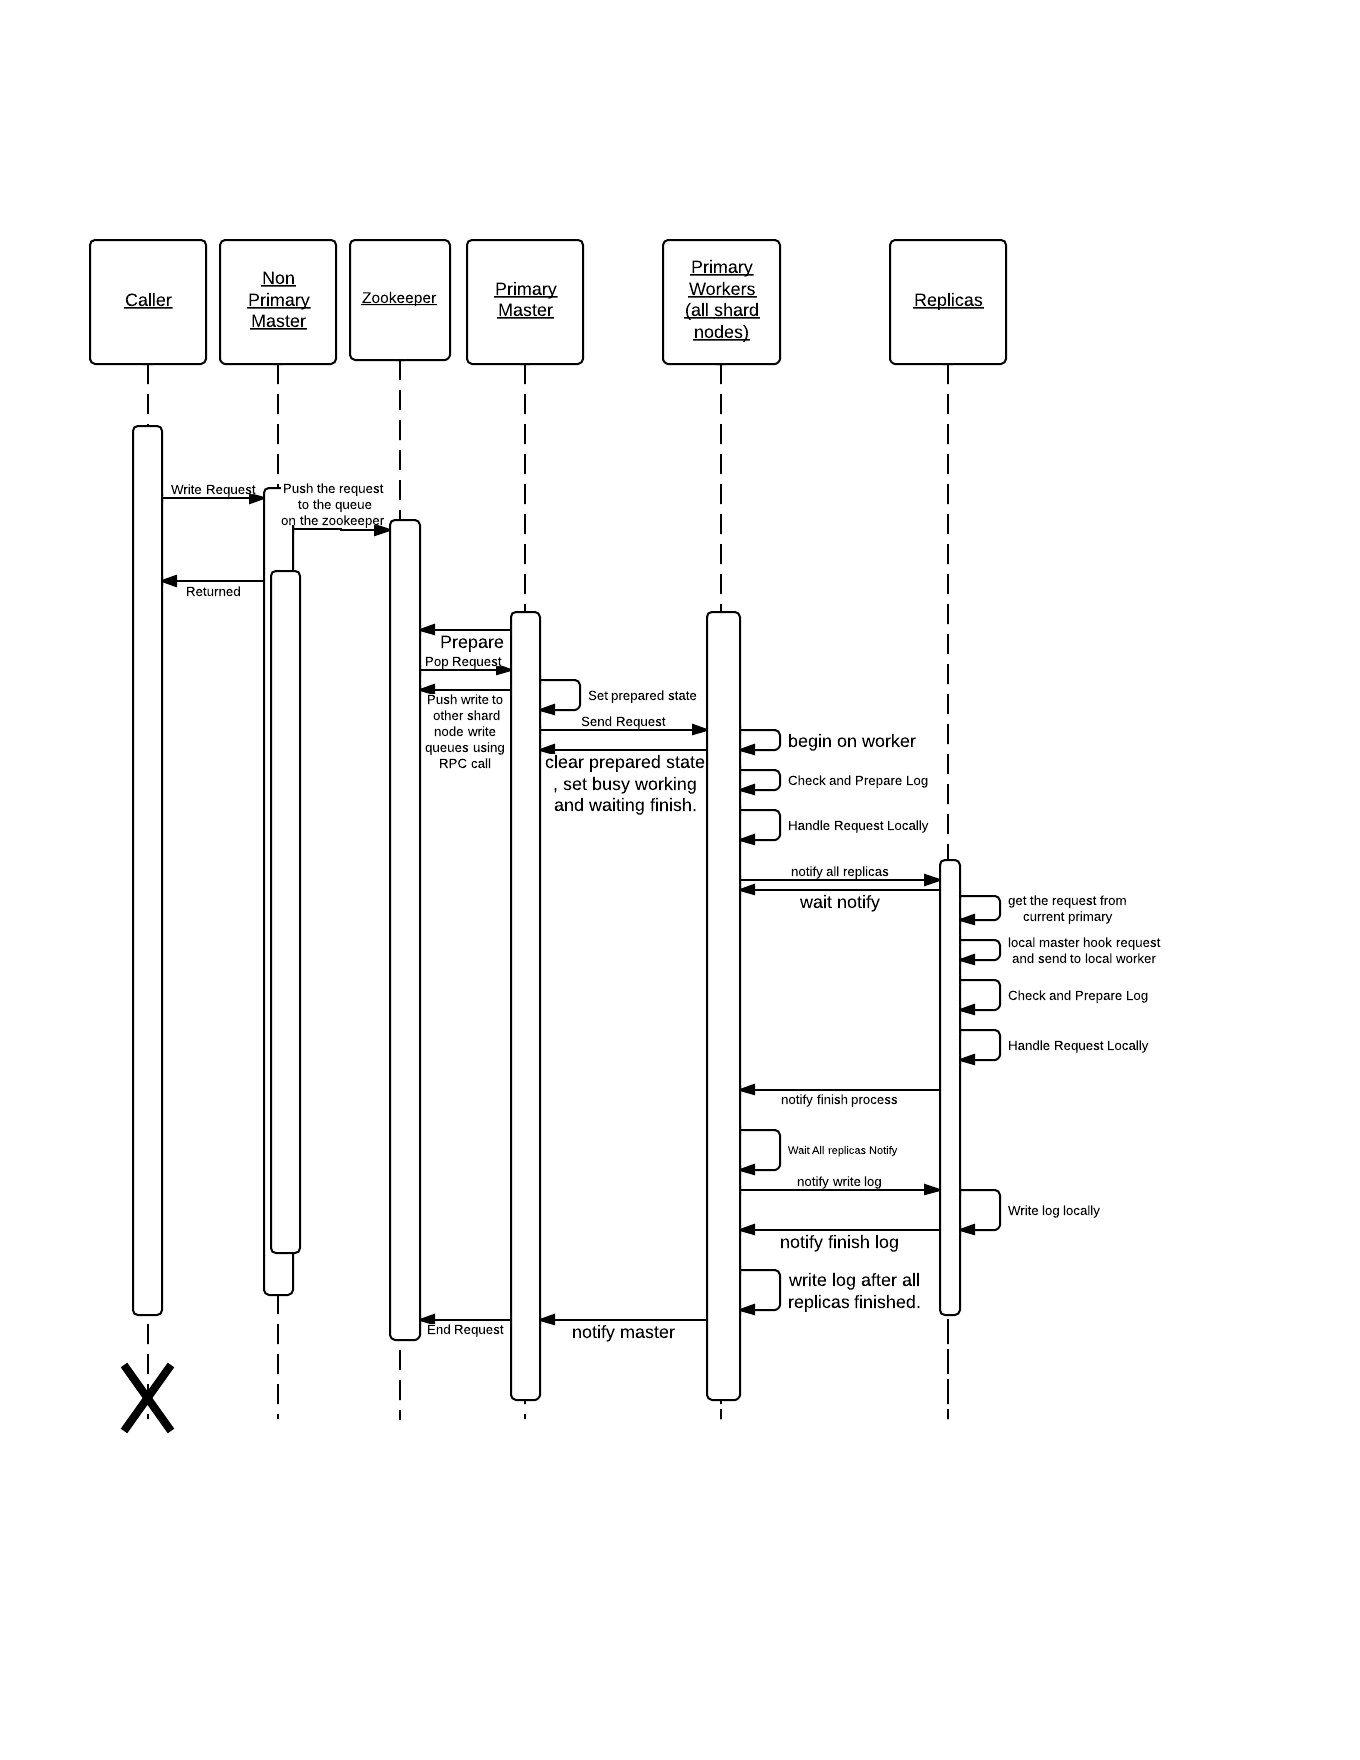
\includegraphics[width=.90\textwidth]{Figures/WriteRequestProcess.png}
  \caption{Write request handling Flow}\label{fig:writeprocess}
\end{figure}

Figure \ref{fig:writeprocess} has shown the working flow of the write request:
\begin{enumerate}
 \item A client caller send write request to one of node in the specific replica set on distributed sf1r.
 \item The master part on the node will push the request to the write queue on zookeeper. For each replica set it has a standalone write queue on the zookeeper for its own.
 \item The primary node will be notified and try to get the new write from zookeeper. If success, the master part on primary node will set the prepared state and pop the write request from the queue.
 \item If the write request should be distributed to other shard workers, it will be pushed to the write queue belong to that shard node.
 \item The primary shard worker begin process on local. After finished on primary worker, it will notify other nodes in the same replica set by updating the zookeeper nodedata. Then the primary worker will wait all secondary nodes until finished or down by accidentally.
 \item The secondary worker will be notified by zookeeper while there is a new write from primary. After the secondary worker finished, it will notify the primary by updating the zookeeper nodedata and wait the primary to get ready to write log.
 \item After all secondary finished the write request(or part of them down), the  primary will notify all secondary to write the log.
 \item The secondary worker will get notified from primary after all secondary finished write request. Then it will write the log to disk and notify primary that the log has been written.
 \item After all secondary finished writting log, the primary worker will write log to disk and the write request is finished finally.
 \item The primary worker notify the primary master on the same node that it is ready for next new request. And the primary master will check if any new request on the write queue and continue to handle the next write request.
\end{enumerate}

\subsection{Starting Node In Distributed SF1R}
How a node start in distributed sf1r is shown as below: \ref{fig:nodestart}. Starting a node will add a secondary to the replica set if there is already a primary, otherwise the starting node will enter the replica set as a primary.

\begin{figure}[!ht]\centering
  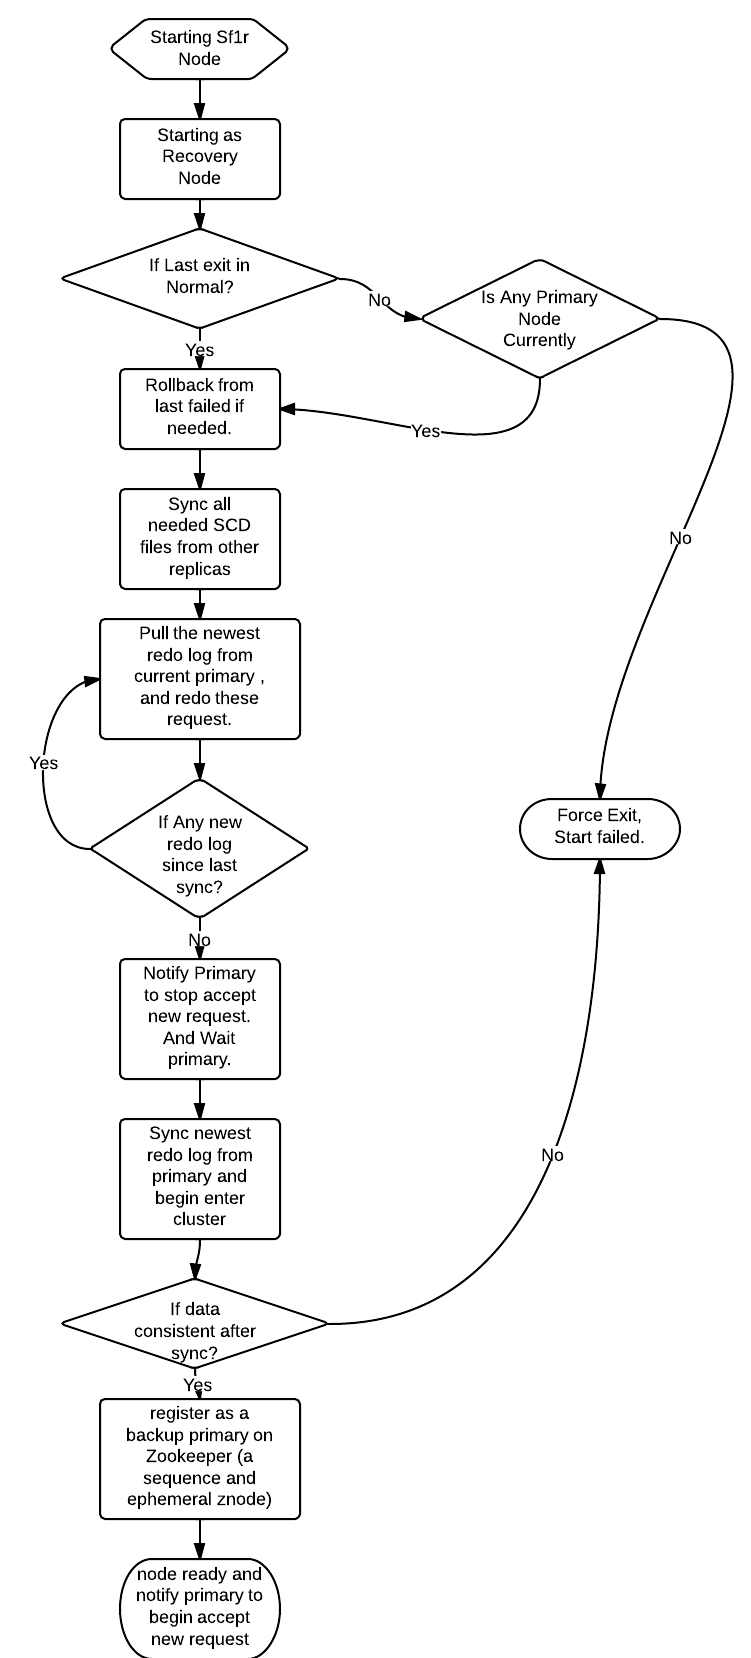
\includegraphics[width=.60\textwidth]{Figures/nodestart.png}
  \caption{Starting of a node}\label{fig:nodestart}
\end{figure}

\begin{enumerate}
 \item \emph{Staring node as primary}\newline
Each distributed node will be registered as a backup primary node in the same replica set on the zookeeper. The first backup primary node in the replica set will be treated as primary.

  \begin{itemize}
   \item Check data: while starting, the node will check whether local data is ok by checking if some flag file exists on local. If last down by accidentally, the node can not be started as primary. Because we can not identify the correctness of the local data without checking by comparing with the other node.
   \item Register as backup primary: After checking data, the first node will start and register a backup primary in the replica set. Because this is the first backup primary, it will be treated as the current primary. The start is finished at last.
  \end{itemize}

 \item \emph{Starting as secondary}\newline
After the first node in the replica set started, all other nodes will be started as secondary.

 \begin{itemize}
 \item Recover: If last exit is normal, no recovery needed. Otherwise, the secondary will restore the data from the newest backup.
 \item Sync to Newest log: After recovery finished, the secondary will pull new log data from primary, and redo the log since last down. After synced to the newest log, the secondary will notify the primary to stop accecpt new request and begin to enter cluster.
 \item Check consistent: If primary agreed the enter of secondary, the secondary will check the data consistent with primary by computing the CRC of the collection data files. If the consistent finished success the node starting as secondary is done at last. Otherwise, the secondary node will fail to start.
 \end{itemize}
 
\end{enumerate}

\subsection{Failing in Distributed SF1R}
In distributed sf1r, there are many cases to cause a failing node. Basically, there are two major fails: primary fail and non-primary fail. Beside, because the zookeeper is used, we need handle the zookeeper connection lost as one kind of fail. The handle of fail is shown in Fig \ref{fig:nodefail}.
\subsubsection{Abort write request}
If the write request failed to finished, the node need rollback to the state before write. This is aborting a write request.
\begin{itemize}
\item When abort hanppen: Abort may happen if the primary failed to finish or a secondary send abort request to primary. The expired session on zookeeper connection while running request will also trigger the aborting. 
\item How to abort: While aborting triggered, the primary node will notify all secondary nodes to abort the request. If the secondary node did not begin to run the write, the abort can ignore since no write happen on the node. Otherwise, the secondary node will do the aborting and notify primary after aborting finished. While aborting on the local node, it will find the latest backup and restore data from it. After that the node will redo the logs between the latest backup and current failed state. By redoing the log, the node can restore state to the old state before the failed write actually running.
\end{itemize}
\subsubsection{Auto failover and recover}
The master will be notified if the fail node is in the watching list of master and the master will try to failover this node by using the backup node with the same nodeid in other replica set. If the fail node restarts later, the master will recover this node.
\subsubsection{Primary Fail}
Current primary fail will trigger a backup primary to begin electing and the backup primary will take the charge of primary if its log is newest.
\begin{enumerate}

\item Primary fail while idle: While idle, the primary fail will notify all replicas in the same replica set and the first backup primary will become new primary and notify all other replicas by updating self state to electing. The other backup nodes will just update the current primary info and notify the new primary that I am ready to follow the new primary. After all other nodes followed the new primary, the new primary will end the electing and ready for the next new write request.
\item Primary fail while write request running local: If the primary failed while running the write request but not finished yet. Because the other nodes in the replica set haven't began to run the write, we can handle it just the same as case 1.
\item Primary fail While write request finished local: In this case, some of the secondary nodes have already begun to run write request on the node. So we need abort the current write request if the node has begun and after aborting the node will reenter the cluster to sync to the new primary. If the node has not yet start to run the write, it can begin electing the same as case 1.
\item Primary fail while ready to write log: In this case, all secondary nodes have already finished write request, but not all secondary nodes finished the log. This is almost the same as the case 3 except the node finished log do not need to abort the current write request. All others not finished log need abort request and re-enter cluster.
\item Primary fail while electing: In this case, it means the current primary failed and the first backup also failed while trying to become new primary. It is almost the same as the case 1 except the second backup take charge of the new primary.
\item Primary fail while others recovering: In this case, the recovering node need follow the new primary and redo recovering from the mew primary. The nodes not recovering can be handled just like the other case in 1-5.
\end{enumerate}

In all case above, the node re-enter cluster if the log is fall behind others. The newest log id will be updated to zookeeper once the node finished log.

\subsubsection{Non-Primary Fail}
\begin{enumerate}

\item Non-Primary fail while idle: Nothing will happen except auto failover on master since no write running.
\item Non-Primary fail while write request running local: The primary will stop waiting this fail node and check if others finished the write request.
\item Non-Primary fail while recovering: The primary will stop waiting this node to enter cluster and check if any new write request can be handled.
\item Non-Primary fail while electing: The new primary will stop waiting this node to follow itself and check if others followed it.

\end{enumerate}

\begin{figure}[!ht]\centering
  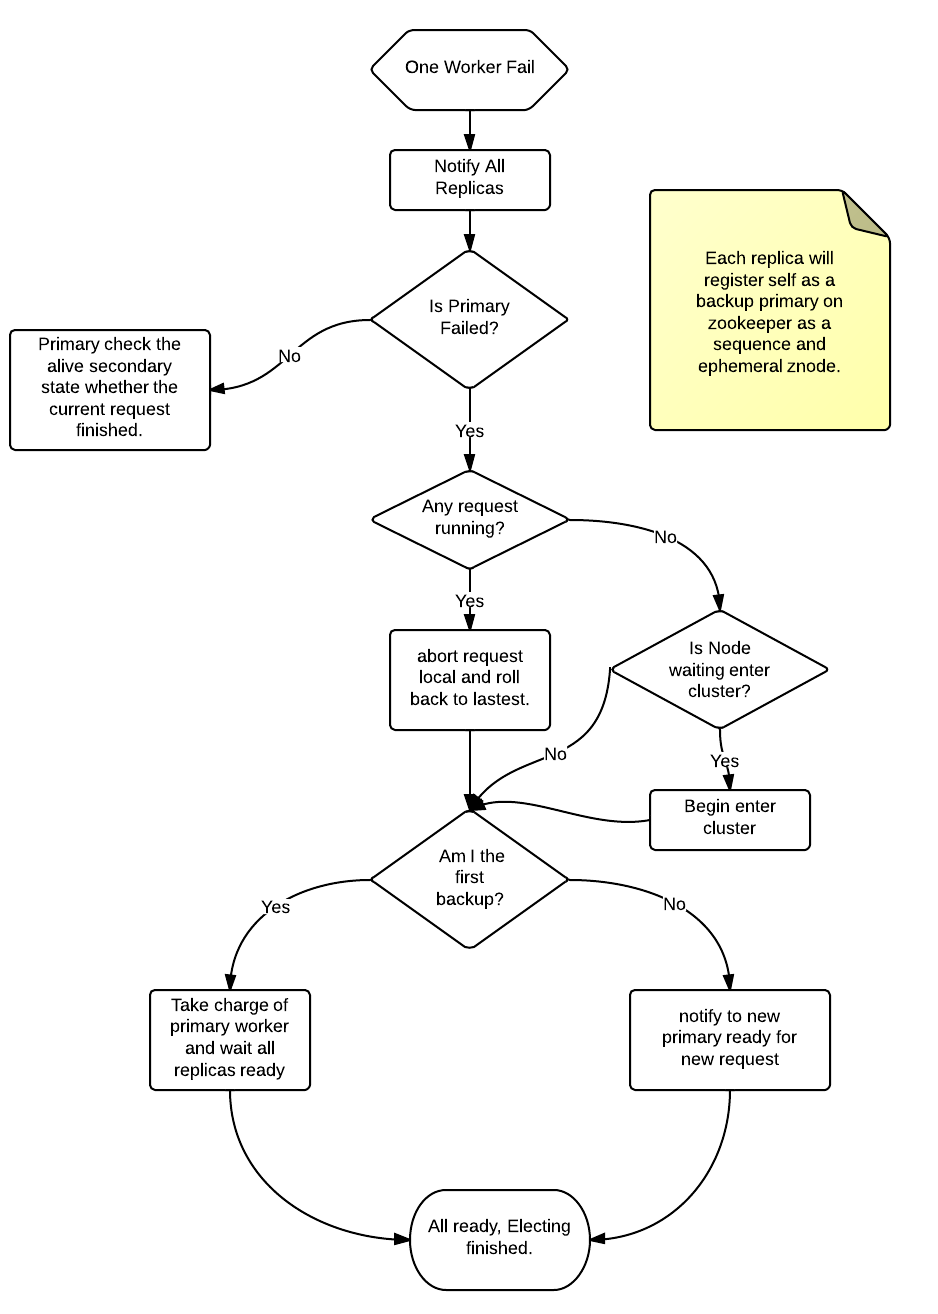
\includegraphics[width=.60\textwidth]{Figures/NodeFail.png}
  \caption{Fail of a node}\label{fig:nodefail}
\end{figure}

\subsubsection{ZooKeeper Connection Lost}
ZooKeeper will lost connection by auto-reconnect or expired session. This may happen while network is unstable or zookeeper server is restarting.
\begin{itemize}
\item Auto-reconnect: In this case, the zookeeper will make sure all nodes created by self keep the same after auto-reconnected. But we need refresh other nodes state such as primary or other secondary nodes after auto-reconnect finished. If primary node has changed during auto-reconnect, the node need do the same thing just like the primary fail case. If nothing happened during auto-reconnect, the node can continue to run without any change.
\item Expired Session: expired session will cause all zookeeper self-created node and event invalid, so we need reconnect to the zookeeper by hand. After expired, the node will set the state and keep waiting until the node is ready to re-enter cluster. Any unfinished write will be aborted.
\item Optimization for the unstable zookeeper: Sometimes the zookeeper is very unstable and we need do some optimization to avoid the unnecessary change of primary node and the abortion of the running write request. This can be done by checking the primary aliveness so we can make sure the electing only start when the primary is really unreachable. In this way, the temporally lost for the primary will not trigger the primary election or write abortion.  
\end{itemize}
 
\subsection{Async write support}
As described above, the write need keep communicating with zookeeper while doing the write. This will cause much downgrade of write performance if there are many replicas in the replica set because of the network latency. In order to improve the  performance of write, the async write has been implemented to reduce the communication with zookeeper while handling the write request. 
\begin{itemize}
\item Async write on primary node: On primary the write flow is almost the same as sync except the notify to zookeeper has been just ignored. In async write, the primary will pop the write request from zookeeper and handle it locally without notify others and keep going on until no more new write on zookeeper. As we can see, the communication with zookeeper has been reduced to only 1 time. This will greatly improve the write performance and will keep the same even the replica set become larger.
\item Async write on secondary node: Since the primary no long notify secondary about the write request, the secondary nodes will pull the redo logs from current primary periodically and redo these logs in the log sync thread. 
\item Drawback of async write: As we can see, the secondary nodes may fall behind from primary node, and if primary failed part of logs may have not synced to other secondary nodes. This will cause write request loss.
\item Recovering in async mode: Since the failed primary may have the logs that other secondary nodes don't have, while the failed primary restarting, the node need check whether the log is newer that current new primary. If restarting with newer log, the node need rollback to old and sync to new primary.

\end{itemize}

\subsection{SF1R lib for distributed SF1R}

\begin{figure}[!ht]\centering
  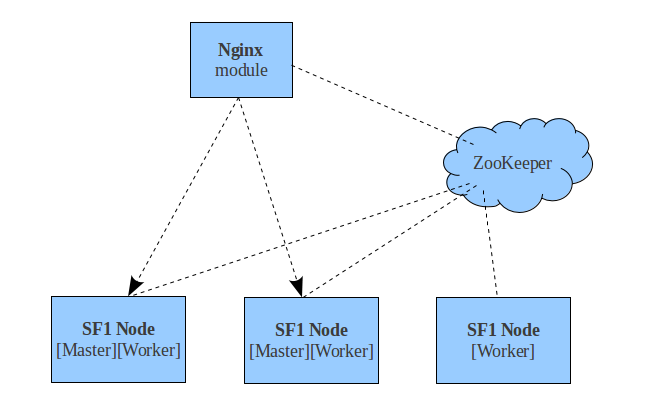
\includegraphics[width=.60\textwidth]{Figures/nginx-sf1rlib.png}
  \caption{The SF1R lib for nginx}\label{fig:sf1rlib}
\end{figure}

The SF1R lib in Fig \ref{fig:sf1rlib} is used by the distributed nginx. By using this sf1r-lib the client can send request with no need for knowing the topology in the distributed sf1r. This client lib will find the correct sf1r node in topology automatically and send the request to it. The client lib update the topology by using the zookeeper connection and any changes from zookeeper will be notified.
  
\begin{itemize}
\item Support For Separating read and write: Currently, the distributed sf1r node will write the current busy state to the zookeeper while the busy state changed. By reading the busy state from zookeeper node we can temporally disable the read from the node who is busy writing. In this way, we can route the read request and write request to different nodes to implement separating the read and write.
\end{itemize}

\subsection{The Sharding for the huge data}
While the data growing rapidly, the single node can not handle all the data anymore. Then we need do the sharding of the data to put the data across several nodes.
\begin{itemize}
\item Benefit: improve read/write performance.
 Concurrently read and write on different nodes is more effective than multi-thread r/w on the single node because there is no CPU contention.
\item What to think: The first thing is load balancing, we should make sure all sharding nodes are handling the average work. The second thing is to handle the add/remove sharding nodes easily since the data may grow rapidly.
\item How to do: Using consistent hashing to keep data balance among all sharding nodes and avoid too much data migrate while changing the sharding nodes topology. Pick up the searching worker one by one to balance the read request among them.
\end{itemize} 


\section{Developer Guide}
Because all the write request will be handled on primary first and send to all secondary nodes from primary, the new write request need some adjustment to be adopted by distributed sf1r. Most work has been done and we can add new write simply follow as below step:

\subsection{Add new write api}

\begin{enumerate}

\item add the controller+action string in the function initWriteRequestSet in the RequestLog.cpp file.
\item if the write api is in the controller that derived from Sf1Controller, then most work will be done OK in base class. If not, you need handle it yourself.
\item If the api will execute on all shard workers, you need push the write request to the queues of other shard workers. (See the index write request in the class IndexTaskService for example.)
\item In the write request handler, coding as below:
\begin{lstlisting}[language=C]
// check valid first.
DISTRIBUTE_WRITE_BEGIN;
DISTRIBUTE_WRITE_CHECK_VALID_RETURN;
// do pre-check without modify any collection data. 
if (precheckfailed())
{
    return false;
}

// prepare request log before actually modify the collection data.
CreateOrUpdateDocReqLog reqlog;
reqlog.timestamp = Utilities::createTimeStamp();
if(!distributereqhooker->prepare(ReqCreateOrUpdate_Doc, reqlog))
{
    LOG(ERROR) << "prepare failed in " << __FUNCTION__;
    return false;
}

// do modify collection data.
ret = modify_data();
if (!ret)
{
    return false;
}
// flush data to make sure data write to disk.
flush();

DISTRIBUTE_WRITE_FINISH(ret, reqlog);
return ret;
\end{lstlisting}
\item Make sure the controller and handler will execute in sync.
\item If an api will call another write api, you should set the chain status properly.
\item Define a new req log type in RequestLog.h if necessary and set for rollback and backup action in DistributeRequestHooker.cpp file.

\end{enumerate}

\subsection{Add new write cron job}
In order to run cron job in distributed mode, the cron job need a job name cronJobName for each cron job and each cron job just do one job. cronJob task is a function with calltype parameter. You should write cron job function as below:
\begin{lstlisting}[language=C]
void RecommendTaskService::cronJob_(int calltype)
{
    if (cronExpression.matchesnow() || calltype > 0)
    {
        // check if need to put the job to distributed sf1r write queue.
        if(calltype == 0 && NodeManagerBase::get()->isDistributed())
        {
            if (NodeManagerBase::get()->isPrimary())
            {
                MasterManagerBase::get()->pushWriteReq(cronJobName_, "cron");
                LOG(INFO) << "push cron job to queue on primary : " << cronJobName_;
            }
            else
                LOG(INFO) << "cron job ignored on replica: " << cronJobName_;
            return;
        }
        // check for valid
        DISTRIBUTE_WRITE_BEGIN;
        DISTRIBUTE_WRITE_CHECK_VALID_RETURN;
        // prepare the log for cron job.
        CronJobReqLog reqlog;
        reqlog.cron_time = Utilities::createTimeStamp();
        if (!DistributeRequestHooker::get()->prepare(Req_CronJob, reqlog))
        {
            LOG(ERROR) << "!!!! failed running cron job. : " << cronJobName_ << std::endl;
            return;
        }
        //do the job task here. and flush data after job finished. 
        bool ret = DoJob();
        flush();
        //finish job
        DISTRIBUTE_WRITE_FINISH(ret);
    }
}
\end{lstlisting}

\subsection{Add new write callback}
The write callback is used for the write without any write api or cronJob. You can add/remove a write callback with an identify string and call it as below :

\begin{lstlisting}[language=C]

// add new callback.
DistributeDriver::get()->addCallbackWriteHandler(collection_ + "_callBackFuncName",
    boost::bind(&CallbackObj::callbackFunc, this, _1));

// removing the callback
DistributeDriver::get()->removeCallbackWriteHandler(collection_ + "_callBackFuncName");

// call callback by push the specific data.
DistributeDriver::get()->pushCallbackWrite(reqloghead.req_json_data, reqdata);

\end{lstlisting}

The callbackFunc should have the protocol as below and should be with the log type ReqCallback:
\begin{lstlisting}[language=C]
bool callbackFunc(int calltype);
\end{lstlisting}

The calltype will be used to tell who is calling this callback. In the callback you should code just like the write request api handler.

\subsection{Auto test}
Currently, the distributed sf1r support auto test for new write request. The auto test will try all possible fail case to check if data is consistent after the write request.

For each write request api, you can add the test json request body to the autotest directory. All the json file under it will be tested in all kinds of node fails to make sure after the write request we  get the consistent data.

If you want some node fail at the some test point, you can do
\begin{lstlisting}[language=C]
echo failtype > distribute_test.conf 
\end{lstlisting}
under the working directory. the \emph{failtype}  here stand for the kind of test point at which line the sf1r will fail. Currently all test points are shown as below:
\begin{lstlisting}[language=C]
enum TestFailType
{
    NoAnyTest = 0,
    NoFail,
    PrimaryFail_At_Electing,
    PrimaryFail_At_BeginReqProcess,
    PrimaryFail_At_PrepareFinished,
    PrimaryFail_At_ReqProcessing,
    PrimaryFail_At_NotifyMasterReadyForNew,
    PrimaryFail_At_AbortReq,
    PrimaryFail_At_FinishReqLocal,
    PrimaryFail_At_Wait_Replica_Abort,
    PrimaryFail_At_Wait_Replica_FinishReq,
    PrimaryFail_At_Wait_Replica_FinishReqLog,
    PrimaryFail_At_Wait_Replica_Recovery,
    PrimaryFail_At_Master_PrepareWrite,
    PrimaryFail_At_Master_checkForNewWrite,

    ReplicaFail_Begin = 30,
    ReplicaFail_At_Electing,
    ReplicaFail_At_Recovering,
    ReplicaFail_At_BeginReqProcess,
    ReplicaFail_At_PrepareFinished,
    ReplicaFail_At_ReqProcessing,
    ReplicaFail_At_Waiting_Primary,
    ReplicaFail_At_Waiting_Primary_Abort,
    ReplicaFail_At_AbortReq,
    ReplicaFail_At_FinishReqLocal,
    ReplicaFail_At_UnpackPrimaryReq,
    ReplicaFail_At_Waiting_Recovery,

    OtherFail_Begin = 60,
    Fail_At_AfterEnterCluster,
    Fail_At_CopyRemove_File,

    FalseReturn_Test_Begin = 70,
    FalseReturn_At_UnPack,
    FalseReturn_At_LocalFinished,
};

\end{lstlisting}

\section{Operation Note}
\subsection{Configuration}
A simple sample configuration is as below:

SF1R Node1, work as Master and Shard Worker 1. For this Master, it provides multiple collections, "b5mp" is distributed to two shard workers.

part of sf1config.xml
\begin{lstlisting}
    <DistributedTopology enable="y">
      <CurrentSf1rNode nodeid="1" replicaid="1">
        <!--master names for B5M are www|stage|beta-->
        <MasterServer enable="y" name="undefined" />
        <WorkerServer enable="y" />
      </CurrentSf1rNode>
    </DistributedTopology>
\end{lstlisting}

part of b5mp.xml
\begin{lstlisting}
    <IndexBundle>
      <ShardSchema>
        <ShardKey name="DOCID" />
        <DistributedService type="search" shardids="1,2" />
        <DistributedService type="recommend" shardids="1,2" />
      </ShardSchema>
      ...
    </IndexBundle>
\end{lstlisting}

SF1R Node2, work as Master and Shard Worker2 (with shard 2).
\begin{lstlisting}
    <DistributedTopology enable="y">
      <CurrentSf1rNode nodeid="2" replicaid="1">
        <MasterServer enable="y" name="undefined" />
        <WorkerServer enable="y" />
      </CurrentSf1rNode>
    </DistributedTopology>
\end{lstlisting}

The \emph{name} in Master Server can be used to tell the difference for independent cluster such as the beta/stage/www cluser.

\subsection{Monitor status}
Some node status will be updated to memory statistical data. If you want to get the running status of distributed sf1r node, you can using the api
\begin{lstlisting}
status/get_distribute_status
\end{lstlisting}
From this we can known the current primary host and how many write request processed and etc..

\subsection{Update SF1R}
The update can have two major cases: simple update and update to new cluster. The simple update will happen while the update is compatible with old node, otherwise update to new cluster is needed.
\begin{itemize}
\item Update config: replace the config file on current primary node and send the api command
\begin{lstlisting}
collection/update_collection_conf 
\end{lstlisting}
After this the updated config will auto deliver to other replicas in the replica set.
\item Simple update: If the data or code is compatible with the old one, we can do simple update. Just using the script below:
\begin{lstlisting}
distribute_tools.sh simple_update new-sf1r-tar-file
\end{lstlisting}
and wait until the updating node can serve as the new master or worker.

\item Update to new cluster: update to new cluster is needed while the new is no longer compatible with the old. We can do this one by one as follow : 
\begin{enumerate}

\item Chose one node in the replica set and run the script :
\begin{lstlisting}
distribute_tools.sh update_to_newcluster new-sf1r-tar-file new-clusterid
\end{lstlisting}
\item Rebuild data if needed by using the api.
\item Backup node data. Using api
\begin{lstlisting}
collection/backup_all
\end{lstlisting}
to generate the backup data on the current node.
\item Copy the backup data to other replicas and update the left nodes one by one. On the other nodes, using the script 
\begin{lstlisting}
distribute_tools.sh rollback new-clusterid
\end{lstlisting}
to restore the data from the copied backup data. After all nodes have finished, the update to new cluster is done.

\end{enumerate}
\end{itemize}
\subsection{Handle Unexpected down}
The node in distributed sf1r may be down at any time. After started, the node will set a force exit flag file and this flag file will be removed if the node is stopped normally. While starting, if the force exit flag exists, we treat it as an accident down. In this case we will restore the data from the latest backup and sync to newest from current primary.

While running the write request, the node will set a rollback flag file to indicate the current running request with the request id. If the write failed to finish, we can know which state we will rollback to. If the rollback file is empty it will rollback to the latest backup.

If all nodes in the replica set are down, we need check the log data carefully. We need find out which node has the newest log data and start this node as the first node in the replica set.

%----------------------------------------------------------------------------------------
%	THESIS CONTENT - APPENDICES
%----------------------------------------------------------------------------------------

\addtocontents{toc}{\vspace{2em}} % Add a gap in the Contents, for aesthetics

%\appendix % Cue to tell LaTeX that the following 'chapters' are Appendices

% Include the appendices of the thesis as separate files from the Appendices folder
% Uncomment the lines as you write the Appendices

%\input{Appendices/AppendixA}
%\input{Appendices/AppendixB}
%\input{Appendices/AppendixC}

\addtocontents{toc}{\vspace{2em}} % Add a gap in the Contents, for aesthetics

%----------------------------------------------------------------------------------------
%	BIBLIOGRAPHY
%----------------------------------------------------------------------------------------

\label{Bibliography}

\lhead{\emph{Bibliography}} % Change the page header to say "Bibliography"

\bibliographystyle{unsrtnat} % Use the "unsrtnat" BibTeX style for formatting the Bibliography

\bibliography{Bibliography} % The references (bibliography) information are stored in the file named "Bibliography.bib"

\end{document}
